\documentclass[a4paper,11pt]{book}

\usepackage[utf8]{inputenc}
\usepackage[italian]{babel}
\usepackage[T1]{fontenc}
\usepackage[letterpaper,top=2cm,bottom=2cm,left=3cm,right=3cm,marginparwidth=1.75cm]{geometry}

% Useful packages
\usepackage{amsmath}
\usepackage{graphicx}
\usepackage[colorlinks=true, allcolors=blue]{hyperref}
\usepackage{listings}
\usepackage{amsthm}
\usepackage{amssymb}

\usepackage{algorithm}
\usepackage{algpseudocode}

\theoremstyle{plain}
\newtheorem{theorem}{Teorema}[chapter]
\theoremstyle{plain}
\newtheorem{lemma}{Lemma}[chapter]
\theoremstyle{definition}
\newtheorem{definition}{Definizione}[chapter]

\usepackage{float}

\title{Crittografia}

\begin{document}
\maketitle

\thispagestyle{empty}

\tableofcontents

\thispagestyle{empty}
	
\cleardoublepage %%%% Add this one here!
\pagenumbering{arabic}

\chapter{Introduzione}
\label{chapter1}

\paragraph*{Crittografia} Nasconde il contenuto del messaggio, ma non l'esistenza dello stesso.

\paragraph*{Stenografia} Nasconde l'esistenza del messaggio (es tecniche: inchiostro invisibile, codifico il messaggio nei bit meno significativi dell'immagine che non sono visibili a occhio nudo). Se qualcuno scopre la tecnica che nasconde il messaggio, allora tutti i messaggi che usano quella tecnica diventano visibili.

\paragraph*{Sistema sicuro} Non esiste un concetto assoluto di sicurezza, ma si può dire che un sistema è sicuro quando il costo necessario a romperlo è superiore al vantaggio economico che si otterrebbe/al danno che si produrrebbe.

\section{Breve storia della crittografia}

\paragraph*{Cifrario di Cesare} Uno dei primi metodi crittografici della storia è quello di \textbf{Cesare}. Si basa sullo shift dell'alfabeto di $n$ posizioni. La chiave corrisponde alla prima coppia di lettere dell'alfabeto originale e traslato (es: la chiave è AD, quindi per decifrare il messaggio devo prendere la lettera che corrisponde a 3 posizioni indietro rispetto a quella scritta nel messaggio cifrato -la lettera D cifrata corrisponderà alla lettera A-).

Si tratta di una cifratura facilmente attaccabile in quanto le \textbf{possibili chiavi} sono solo 26 (\textbf{tutti gli shift dell'alfabeto}).

Un attacco di questo genere (testo tutti i possibili shift) si chiama attacco di forza bruta: testo tutte le chiavi possibili finché trovo quella corretta.

\paragraph{Permutazione arbitraria dell'alfabeto} Un'evoluzione di questo metodo di cifratura è la \textbf{permutazione arbitraria}. Questo metodo si basa sulla permutazione totale dell'alfabeto, piuttosto che sul suo semplice shift. In questo caso la \textbf{chiave} è \textbf{alfabeto permutato}.

Le possibili chiavi sono $[26!]$ (50 anni fa non era facilmente attaccabile da attacchi di forza bruta a causa dei pc poco potenti). Questa cifratura è attaccabile con l'\textbf{analisi delle frequenze}\footnote{L'analisi delle frequenze è lo studio della frequenza di utilizzo delle lettere o gruppi di lettere in un testo cifrato. Questo metodo si basa sul fatto che in ogni lingua la frequenza di uso di ogni lettera è piuttosto determinata; questo è vero in modo rigoroso solo per testi lunghi, ma spesso testi anche corti hanno frequenze non molto diverse da quelle previste. 

Tramite questa analisi è possibile inoltre determinare anche la lingua del messaggio, in quanto ogni lingua ha delle frequenze specifiche (tralasciando le lingue orientali).}. 
Nel caso si utilizzi un attacco a forza bruta (automatizzato dal pc), è possibile capire che se ho raggiunto il risultato corretto sempre tramite l'analisi delle frequenze. 

\paragraph{Counter all'analisi delle frequenze} Si propose di lavorare non più con una singola lettera, ma con coppie di lettere. In questo modo ad ogni lettera cifrata potevano corrispondere 2 lettere in chiaro. Uno degli approcci utilizzati è il seguente:

\begin{table}[H]
\centering
\begin{tabular}{|c|c|c|c|c|}
\hline
& & & & &
\hline 
& & & & &
\hline 
& & & & &
\hline 
& & & & &
\hline 
& & & & &
\hline 
\end{tabular}
\end{table}

\noindent Supponiamo di avere una tabella $5 \times 5$ che andrà a contenere una password che sarà la chiave. Usiamo la parola \textit{MONARCHY}. Nel caso la password contenga lettere ripetute, le ripetizioni vengono saltate, in modo che ogni lettera compaia una sola volta.

\begin{table}[H]
\centering
\begin{tabular}{|c|c|c|c|c|}
\hline
M & O & N & A & R &
\hline 
C & H & Y & & &
\hline 
& & & & &
\hline 
& & & & &
\hline 
& & & & &
\hline 
\end{tabular}
\end{table}

\noindent A questo punto procediamo inserendo le lettere dell'alfabeto mancanti, saltando ovviamente quelle già inserite. Consideriamo la lettera I uguale alla lettera J (ho 25 posti e le lettere sono 26).

\begin{table}[H]
\centering
\begin{tabular}{|c|c|c|c|c|}
\hline
M & O & N & A & R &
\hline 
C & H & Y & B & D &
\hline 
E & F & G & I/J & K &
\hline 
L & P & Q & S & T &
\hline 
U & V & W & X & Z &
\hline 
\end{tabular}
\end{table}

\noindent Possiamo procedere ora con la codifica, lavorando sulle coppie di lettere. Le regole da seguire sono:
\begin{itemize}
    \item Se la coppia di lettere da cifrare appartiene alla stessa riga nella tabella, si prenderà la lettera successiva nella riga, procedendo in maniera circolare.
    
    Esempio: Supponiamo di dover cifrare la coppia AR. Nella tabella AR appartiene alla stessa riga, quindi uso la regola sopra. La lettera A corrisponderà alla lettera R (mi sposto di una posizione), mentre la lettera R corrisponderà alla lettera M (essendo la fin della riga, la posizione successiva è l'inizio della riga stessa).
    
    Quindi:
    \begin{center}
        AR $\longrightarrow$ RM\\
        OA $\longrightarrow$ RN
    \end{center}
    
    \item Se la coppia appartiene alla stessa colonna, lavoro come nel primo caso, solo che qui mi sposto verso il basso sulla colonna.

    Esempio:
    \begin{center}
        MU $\longrightarrow$ CM
    \end{center}
    
    \item Se la coppia appartiene a righe e colonne diverse, la prima lettera si sposterà nella colonna della seconda e viceversa.
    
    Esempio:
    \begin{center}
        PB $\longrightarrow$ SH\\
        EA $\longrightarrow$ IM oppure JM
    \end{center}
    
\end{itemize}

\noindent Anche questo metodo è comunque attaccabile con l'analisi delle frequenze, in quanto, sebbene la codifica di una lettera dipende dall'altra della coppia (e quindi non valore più il caso di \textit{a lettera uguale corrisponde lettera uguale}), vale il caso in cui "a coppia uguale corrisponde coppia uguale" e anche le coppie di lettere di una lingua hanno le loro frequenze.

\paragraph{Cifrario di Vigenère} Il cifrario di Vigenère riprende l'idea del cifrario di Cesare: presa una chiave (es: \textit{key}), si ripete la chiave tante volte quanto è lungo il testo (eventualmente troncando l'ultima ripetizione), e si codifica la lettera con il corrispondete cifrario di Cesare. \\
	
\noindent
K E Y K E Y K E Y K E Y \\
P R O V A D I T E S T O \\
	
\noindent La prima lettera del cipher text sarà la lettera ottenuta dal cifrario di Cesare di chiave AP, la seconda con la chiave AR e così via.
	
Anche questo cifrario è semplice da attaccare, si parte dalla divisione del ciphertext in gruppi di lunghezza pari a quella della chiave, e si esegue l'analisi delle frequenze su ogni gruppo. Nel caso in cui non si conosca la lunghezza della chiave, si può semplicemente provare tutte le possibili lunghezze della chiave. Ovviamente sarà necessario un testo di dimensioni maggiori ai precedente per poter effettuare l'analisi. Se la password fosse lunga quanto il testo, l'analisi delle sequenze non sarebbe possibile.
	
\paragraph{One-time pad} Vediamo ora lo schema di Vigenère applicato ad un alfabeto binario. In questo caso il mio alfabeto si compone di soli due simboli: 0 e 1. Posso avere solo 4 casi di chiave-testo:
\begin{align*}
Key \rightarrow &1 0 1 0 \\
Text \rightarrow &0 1 0 1 \\
Cyph \rightarrow &0 1 1 0 \\
\end{align*}

\noindent Praticamente applicare questo schema ad un alfabeto binario equivale ad applicare lo XOR tra testo in chiaro e chiave. Per riottenere il plaintext a partire dal cyphertext, mi basta riapplicare lo XOR tra chiave e cyphertext. Riassumendo:
\begin{align*}
    \text{Encryption } E(P, K) = P  \oplus K\\
    \text{Decryption } D(C, K) = C  \oplus K
\end{align*}

\noindent Se ho una chiave lunga quanto il testo e la chiave è scelta in modo casuale (ogni bit del testo è indipendente dalla chiave (viene scelto non conoscendo la chiave)):
\begin{itemize}
    \item La probabilità che il primo bit \textit{b} del cyphertext \textit{c} sia 0 è $\frac{1}{2}$ (lo stesso che sia uno);
    \item La probabilità che il primo bit del cyphertext sia 0 è
        \begin{align*}
            Pr[c = 0] &= Pr[b = 0 \land k = 0] + Pr[b = 1 \land k = 1]\\
                    &= P \cdot \frac{1}{2} + (1-P) \cdot \frac{1}{2}\\
                    &= \frac{1}{2} (P+1-P)\\
                    &= \frac{1}{2}
        \end{align*}
    \noindent Ovvero la probabilità che il cyphertext \textit{c} sia 0 è data dalla probabilità \textit{P} che il bit \textit{b} sia stato scelto con valore 0, moltiplicata la probabilità che il bit \textit{k} della chaive sia stato scelto a 0, sommata alla probabilità che il bit del plaintext \textit{b} sia stato scelto a 1, quindi \textit{P - 1}, moltiplicata la probabilità che \textit{k} sia 1.
\end{itemize}

\noindent Se scelgo la chiave in maniera casuale, a prescindere da come è stato scelto il plaintext, la distribuzione probabilistica sul cyphertext è quella uniforme. Quindi osservando il cyphertext vedo solo una sequenza casuale di bit, che non mi può dire nulla sul plaintext (ogni plaintext è equamente probabile dato il cyphertext). Questo sistema, detto \textbf{one-time pad}, è assolutamente sicuro.

\paragraph{Teorema di Shannon} Per avere un sistema crittografico sicuro, tale per cui a partire dal cyphertext non si può ricavare nulla del plaintext, allora la chiave deve essere tanto lunga quanto il plaintext. 

Secondo questo teorema, i sistemi usati oggi non sarebbero sicuri, in quanto usano chiavi con dimensione inferiore al messaggio scambiato. Per questo l'obiettivo è costruire sistemi dove, sebbene sia possibile ottenere informazioni dal cyphertext, questa operazione diventi troppo complessa (es: richiede molto tempo).
	
\section{Problemi di sicurezza non legati alla crittografia}
La sicurezza del dato non dipende solo dall'affidabilità del protocollo crittografico utilizzato. Rischi di sicurezza possono derivare, ad esempio, anche dalle implementazioni. 

Vediamo il caso dell'IBM 360. Il sistema utilizzava, per il controllo della password, il semplice controllo della stringa (si confronta la prima coppia di lettere e se uguali si passa alla seconda e così via) e memorizza la password in chiaro. Si riuscì a fare in modo che una parte della password inserita per il test finisse in una pagina di memoria, mentre il resto in una seconda pagina che finisce fuori dalla chache. Si faceva quindi partire il confronto e se il sistema ritornava un page fault\footnote{Il page fault è un'eccezione generata quando un processo cerca di accedere a una pagina che è presente nel suo spazio di indirizzamento virtuale, ma che non è presente nella memoria fisica poiché mai stata caricata o perché precedentemente spostata su disco di archiviazione. Tipicamente, il sistema operativo tenta di risolvere il page fault caricando la pagina richiesta nella memoria virtuale oppure terminando il processo in caso di accesso illegale. Il componente hardware che rileva i page fault è il memory management unit, mentre quello software di gestione delle eccezioni è generalmente parte del sistema operativo (kernel). } allora la parte di password scritta nella prima pagina era corretta (se fosse stata errata il controllo si sarebbe fermato prima di raggiungere la seconda pagina, che essendo fuori dalla chache, dà page fault).

Un altro problema legato al controllo tramite confronto delle stringhe è che più lunga è la stringa, maggiore è il tempo necessario per terminare l'operazione. Si potrebbe quindi determinare la lunghezza della stringa contando i microsecondi necessari al completamento del controllo.
\chapter{Crittografia in cascata}
\label{chapter2}

L'idea è di provare a mettere in cascata una serie di sistemi crittografici deboli (es: usando chiavi piccole) per vedere se si riescono a ottenere sistemi più forti. 

\section{Permutazioni in cascata} 
Ho un rullo a due facce. Su ciascuna faccia sono presenti 26 contatti, che rappresentano le 26 lettere dell'alfabeto. Un qualsiasi collegamento interno al cilindro tra le due facce mi rappresenta una possibile permutazione (es: sul lato del plaintest premo il contatto che rappresenta la A e ottengo sull'altro lato, che mi rappresenta il cyphertext la lettera P). Suppongo di scegliere per il rullo la permutazione $\Pi_1$. Collego ora alla faccia del cyphertext del rullo un secondo rullo (che funziona esattamente come il primo) e per lui scelgo la permutazione $\Pi_2$. Aggiungo un terzo rullo collegato alla faccia cyphertext del secondo e scelgo la permutazione $\Pi_3$. Il mio sistema è diventato più resistente? No. La combinazione delle 3 (o anche $n$) permutazioni $\Pi_1 \circ \Pi_2 \circ \Pi_3$ è, alla fine, una permutazione, che sarà identica per ogni lettera del testo che voglio cifrare.

Provo quindi a creare una soluzione più robusta. Decido ora di ruotare il terzo cilindro di una posizione dopo aver codificato ogni lettera del plaintext. Con questa soluzione non ho più una permutazione unica associata all'intero plaintext, ma una per ogni sua lettera, fino ad un massimo di 26 shift, in quanto poi ritorno alla posizione iniziale. Ovviamente, se decido di ruotare il secondo rullo per ogni giro completo, incremento il numero di permutazioni uniche che posso usare ($26^2$).

\section{Enigma} 
Enigma usava un metodo di cifratura molto simile a quello descritto sopra. La sua vulnerabilità non stava tanto nel sistema, ma nel fatto che ogni messaggio scambiato iniziava sempre con lo stesso testo, dal quale gli attaccanti sono riusciti a romperla. Enigma era quindi vulnerabile al \textbf{known plaintext attack}.

\section{Tipi di attacchi} 
Vediamo gli attacchi che un sistema crittografico può affrontare per essere considerato affidabile:
\begin{itemize}
    \item Known cyphertext attack: l'attaccante conosce solo il testo cifrato del messaggio;
    \item Known plaintext attack: l'attaccante conosce il messaggio in chiaro e il relativo cyphertext;
    \item Chosen plaintext attack: l'attaccante sceglie il messaggio da cifrare e analizza il relativo cyphertext;
    \item Adaptive chosen plaintext attack: l'attaccante sceglie il testo di un primo messaggio, analizza il cyphertext ottenuto e in base all'analisi sceglie un nuovo messaggio da cifrare e così via.
\end{itemize}

Se, ad esempio, il sistema è vulnerabile ad un \textit{adaptive chosen plaintext attack}, sarà più affidabile di un sistema che è debole ad un \textit{known cyphertext attack}.

\section{Nascita di DES} 
Col tempo diventa necessario avere un sistema crittografico standard internazionale. Tra le proposte alla fine ne venne scelta una e il protocollo venne chiamata Data Encryption Standard (DES). DES venne costruito con l'idea di durare una ventina d'anni, come è effettivamente stato. DES venne bucato con la \textbf{crittoanalisi differenziale}.

A partire da due input \textit{x} e \textit{y} e i rispettivi cyphertext \textit{E(x, k)} e \textit{E(y, k)} cifrato con chiave \textit{k}, questa analisi confrontava lo XOR degli input con lo XOR dei cyphertext. Praticamente analizzava come le differenze tra i bit di ingresso si propagassero nei bit di uscita. 

\begin{center}
    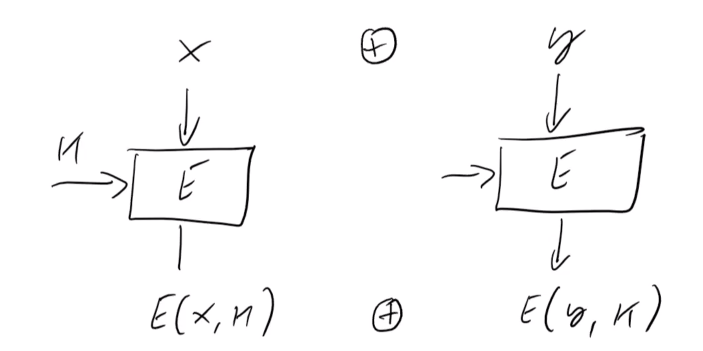
\includegraphics[width=1\textwidth]{images/1.png}
\end{center}

\noindent L'analisi ritornava un'equazione lineare sui bit della chiave \textit{k}, permettendo di costruire alla fine un sistema di equazioni indipendenti a 56 variabili, che rappresentano i 56 bit della chiave usata da DES. Si è scoperto che fissando 12 variabili, era possibile risolvere il sistema, e quindi ottenere la chiave. Di conseguenza, un attaccante non doveva più ricavare 56 bit, ma solo 12 (in quanto gli altri 44 sono ricavabili da questi), riducendo il numero di tentativi necessari per un attacco a forza bruta a solo $2^{12} = 4096$ tentativi.

\noindent Per fare questa analisi è necessario utilizzare un \textit{adaptive chosen plaintext attack}.

\section{Nascita di AES} 
Scoperta la debolezza di DES, si cercarono nuovi protocolli per sostituirlo, che fossero resistenti alle sue vulnerabilità. Venne scelto l'algoritmo che poi venne chiamato Advanced Encryption Standard (AES), che è quello usato oggi. Sostanzialmente è una sequenza di quattro fasi, ognuna delle quali va a contrastare uno degli attacchi noti a DES. Sia per DES che per AES, non esiste una vera e propria dimostrazione che il sistema sia robusto, ma c'è solamente una analisi che dice "ci abbiamo provato in tanti e abbiamo una ragionevole convinzione che saranno robusti almeno per un po' di tempo". 

\paragraph{Fattorizzazione di un numero} In generale, non esiste un modo per costruire un protocollo dove si sa che sia sicuro alla base, ovvero che sappiamo che invulnerabile ad attacchi presenti e futuri, eccetto per one-time pad, dove abbiamo visto che esiste una dimostrazione che funzione ed è sicuro. 

Gli algoritmi attualmente esistenti di fattorizzazione di un numero provano tutti i possibili divisori del numero, ed hanno una complessità esponenziale al numero di bit del numero. Molte persone, appartenenti ad abiti diversi, hanno provato a trovare un algoritmo più ottimizzato, ma senza successo. Verosimilmente un algoritmo efficiente per fattorizzare un numero non verrà trovato. Quindi, se si riuscisse a costruire un crittosistema per il quale è possibile dire che se si trova un algoritmo per attaccarlo allora si è trovato un algoritmo per fattorizzare un numero, allora in questo caso si può dire che l'attaccante non ci possa riuscire. 

\section{Overview di DES}

\begin{center}
    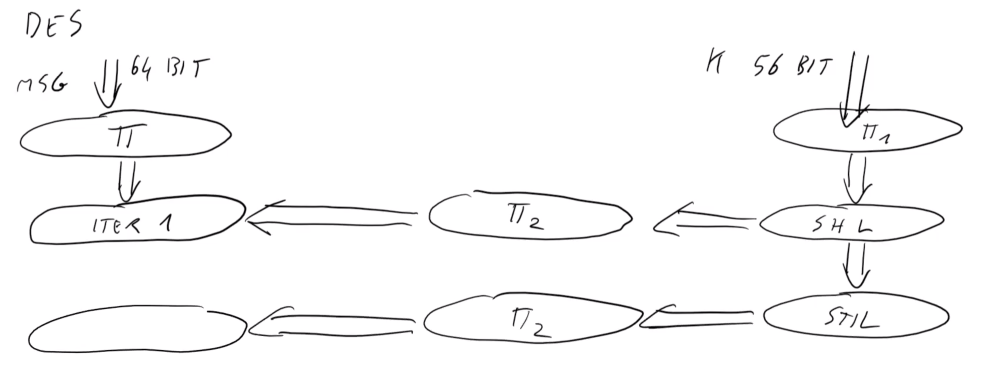
\includegraphics[width=1\textwidth]{images/2.png}
\end{center}

Dato un messaggio di 64 bit e una chiave di 56 bit, DES prevede i seguenti passi:

\begin{enumerate}
    \item Permuto con permutazione $\Pi$ il messaggio;
    \item Permuto la chiave \textit{k} con permutazione $\Pi_1$;
    \item Shifto con rotazione la chiave permutata a sinistra di una posizione;
    \item Applico la permutazione $\Pi_2$ alla chiave shiftata;
    \item Applico la chiave ottenuta al messaggio permutato, utilizzando il meccanismo di \textbf{Feistel};
    \item Ripeto i passi 3, 4 e 5 per 16 volte;
    \item Applico infine al risultato $\Pi^{-1}$, ovvero calcolo ,a permutazione inversa a quella iniziale.
\end{enumerate}

\noindent Le permutazioni usate non aggiungono nulla dal punto di vista della sicurezza del sistema, riguardano infatti l'aspetto fisico del sistema: poiché il sistema è implementato in un chip non è detto, per ragioni di ottimizzazione dello spazio, che contatti di entrata e di uscita si trovino nello stesso ordine.
\\

\noindent Il meccanismo di Feistel è fatto in modo che l'algoritmo di codifica e decodifica siano uguali. Questa soluzione mi costa meno a livello di hardware, in quanto mi basta un solo chip. Le chiavi però devono essere usate, nella decodifica, in ordine inverso rispetto alla codifica. Lo scopo di Feistel era quello di creare uno schema dove algoritmo di codifica e decodifica fossero gli stessi e che fosse applicabile a crittosistemi diversi.

\begin{center}
    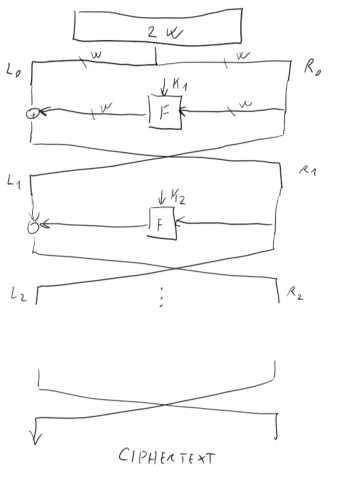
\includegraphics[width=0.5\textwidth]{images/3.png}
\end{center}

Lo schema di Feistel prende in input un flusso di dati in ingresso di dimensione $2W$ (con $W$ numero arbitrario) ed esegue le seguenti operazioni:
\begin{enumerate}
    \item Divide il messaggio iniziale in due messaggi $L_0$ e $R_0$ entrambi di dimensione $W$;
    \item $R_0$ viene applicato ad una funzione qualsiasi $F$, con chiave $k_1$, e produce un nuove messaggio di dimensione sempre $W$;
    \item Il messaggio risultate al punto 2 viene messo in XOR col messaggio $L_0$;
    \item Il messaggio $R_0$ e il messaggio risultatane dal punto 3 vengono scambiati di posizione, diventando il messaggio $L_1$ e $R_1$;
    \item I punti 2, 3 e 4 vengono ripetuti per $n$ volte, utilizzando sempre una chiave diversa ($k_2$, $k_3$, ...);
    \item Eseguo un ultimo scambio tra il messaggio di destra e quello di sinistra, ottenendo il cyphertext.
\end{enumerate}

\noindent La caratteristica interessante di questo schema è che indipendentemente dalla funzione $F$ l'applicazione di questo protocollo a partire dal cyphertext con le chiavi in ordine inverso produce il plaintext. Quindi $F$ può essere qualsiasi funzione. 
\\

\noindent Supponiamo ora di avere il seguente schema di Feistel dicodifica e decodifica, con quattro passi, dove non scambio i due lati, ma ci cambio solo il nome, eccetto per il passo finale.\\

\begin{center}
    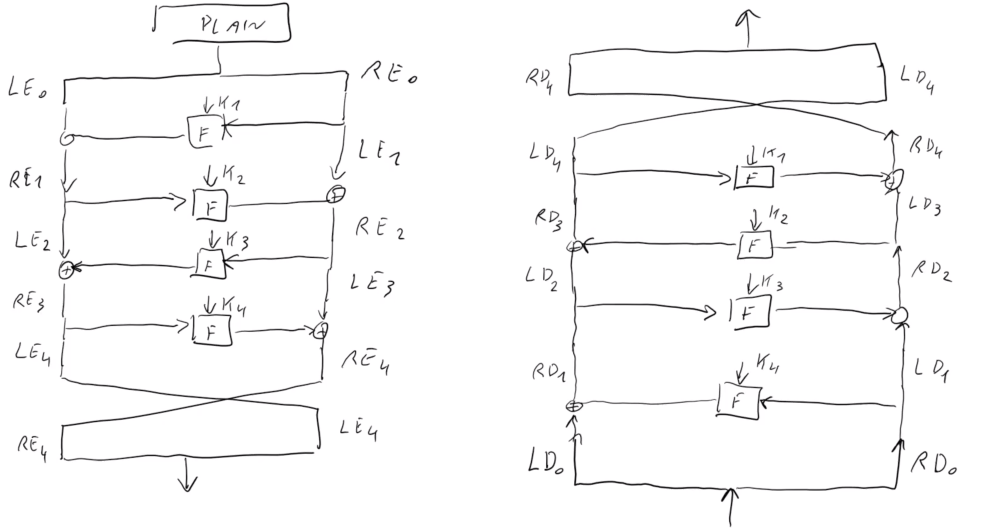
\includegraphics[width=1\textwidth]{images/4.png}
\end{center}

\noindent Dimostriamo ora che i due schemi sono identici:
\begin{align*}
    LD_1 = RD_0 = LE_4 = RE_3\\
    RD_1 = LD_0 \oplus F(K_4, RD_0) &= RE_4 \oplus F(K_4, RE_3)\\
                                    &= LE_3 \oplus F(K_4, RE_3) \oplus F(K_4, RE_3)\\
                                    &= LE_3
\end{align*}      

\noindent Quindi la \textit{Left Decryption 1} equivale alla \textit{Right Encryption 3} e la \textit{Right Decryption 1} equivale alla \textit{Left Encryption 3}. Questa dimostrazione può essere estesa anche ai restanti tre passi, andando a confermare che lo schema di Feistel per codifica e decodifica è lo stesso. 

Come si può vedere, la funzione \textit{F} va solo ad aggiungere confusione; il prodotto del plaintext per la funzione viene automaticamente rimosso durante la decodifica, a prescindere da cosa sia. La \textit{F} ha il compito di rendere difficile la decodifica non conoscendo quale sia la chiave. 

\begin{center}
    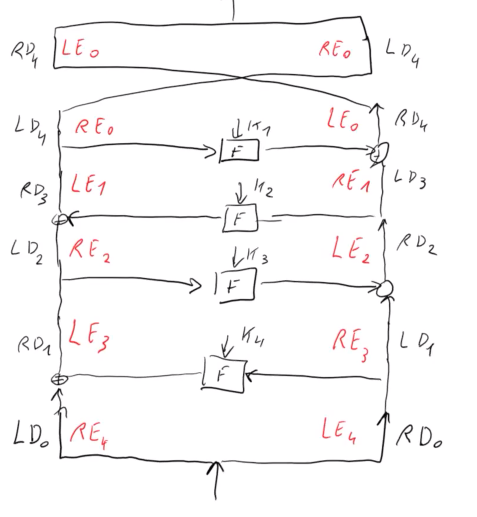
\includegraphics[width=1\textwidth]{images/5.png}
\end{center}

\chapter{Cenni alla teoria dei numeri}
\label{chapter3}

\begin{definition}
Sia \(m \ge 1\) un intero. Gli interi \(a\) e \(b\) sono \textit{congruenti modulo m} se la loro differenza \(a-b\) è divisibile per \(m\). La formula 
\[a \equiv b \pmod m\]
indica che \(a\) e \(b\) sono congruenti in modulo \(m\).
\end{definition}

\noindent\\ Un esempio può essere l'aritmetica delle "ore". Usando il modulo $m = 12$:
\begin{align*}
    6+9=15 \equiv 3 \pmod{12} \hspace{2cm} 2-3=-1 \equiv 11 \pmod{12}
\end{align*}

\noindent I numeri che soddisfano 
\begin{align*}
    a \equiv 0 \pmod m
\end{align*}
\noindent sono tutti i numeri divisibili per $m$, ovvero tutti i suoi multipli $km$.\\

\noindent Dati $m \ge 1$ e $a, b$ interi, allora
\begin{align*}
    a \cdot b = 1 \pmod m
\end{align*}

\noindent se e solo se $GDC(a, m) = 1$.\\

\noindent Dato $GDC(a, m) = 1$ allora esiste un inverso $a^{-1}$ di $a \pmod m$ tale per cui $a^{-1}a \equiv 1 \pmod m$. \\

\noindent \underline{Esempio}: dati $m = 5$ e $a = 2$, $GDC(5, 2) = 1$ e quindi esiste un inverso di $2 \pmod 5$. L'inverso è $3$, in quanto $2\cdot 3 \equiv 1 \pmod 5$.
\\

\noindent Se $a$ diviso $m$ ha quoziente $k$ e resto $r$, allora questo può essere riscritto come:
\begin{align*}
    a = m \cdot k + r \hspace{1cm} \text{con } 0 \le r < m
\end{align*}

\section{Algebra modulo n}
L'insieme $Z_n$ viene definito come l'insieme delle classi di equivalenza $[0]$, $[1]$, $...$, $[n-1]$ di una relazione che dice che ${a}$ è congruente a ${b}$ se e solo se ${a}$ modulo $n$ è uguale a ${b}$ modulo ${n}$, dove il modulo è il resto della divisione per ${n}$:

\begin{align*}
    Z_n = \{[0], [1], [2], ..., [n-1]\}\\
    a \equiv_n b \Longleftrightarrow a \pmod n= b \pmod n
\end{align*}

\noindent Quando ho una relazione di equivalenza posso costruire gli insiemi degli insiemi che sono equivalenti tra di loro. L'insieme degli insiemi che sono equivalenti tra di loro forma una partizione dell'insieme di partenza; gli elementi della partizione vengono chiamati classi di equivalenza e si denotano mettendo tra parentesi quadre \textit{[ ]} un elemento della classe di equivalenza. 

Quindi quando parlo di un'algebra modulo n parlo di un insieme $Z_n$ che è l'insieme delle classi di equivalenza della divisione per n; ogni singola classe di equivalenza può essere rappresentata da un qualsiasi elemento che vi appartiene. Posso infatti anche scrivere:
\begin{align*}
    Z_n = \{0, 1, 2, ..., n-1\}
\end{align*}

\noindent ovvero i primi \textit{n} numeri naturali a partire dallo $0$. La rappresentazione canonica in un'algebra a modulo n è un numero compreso tra $0$ e $n-1$.\\

\noindent\fbox{%
    \parbox{\textwidth}{%
    Il cifrario di Cesare lavora shiftando ogni lettera dell'alfabeto di un numero fissato di posizioni. Lo shift può essere descritto con un'aritmetica modulo $26$:
    \begin{align*}
        (Cyphertext) \equiv (Plaintext\_Letter) + (Secret\_Key) \pmod{26}\\
        (Plaintext\_Letter) \equiv (Cyphertext) - (Secret\_Key) \pmod{26}
    \end{align*}
    }
}

\paragraph*{Numeri razionali} Questo tipo di notazione è già stata usata per definire i numeri razionali, che sono classi di equivalenza su coppie di numeri naturali dove due coppie sono equivalenti se hanno gli stessi prodotti incrociati (prodotto dei medi uguale prodotto degli estremi). 

Ad esempio la coppia ${\frac{a}{b}}$ è un rappresentate delle coppie ${\frac{2a}{2b}}$, ${\frac{3a}{3b}}$ e così via. Tra tutti i possibili rappresentati di una classe ce n'è uno canonico, dove in questo caso è l'oggetto che si ottiene dalla riduzione ai minimi termini.

\subsection{Somma nell'insieme $Z_n$} Definisco ora l'operazione di somma $(Z_n, +)$:
\begin{align*}
    [a] + [b] = [a + b]
\end{align*}

\noindent Questa definizione dice che la somma delle classi di equivalenza di $[a]$ e $[b]$ è uguale alla classe di equivalenza della somma di $a$ e $b$ $[a+b]$. Si considera buona solo se il risultato è indipendente dagli elementi che prendo come rappresentanti delle due classi da sommare. Questa operazione di somma gode di una serie di proprietà:
\begin{itemize}
    \item La somma è commutativa: $\forall a, b: a+b=b+a$;
    \item La somma è associativa: $\forall a, b, c: (a+b)+c=a+(b+c)$;
    \item La somma ammette un elemento neutro $e$: $\exists \ e \forall a: a+e=e+a=a$ con $e= 0 \lor n$. Nell'algebra modulo n vale anche $n$ (e anche $2n$, $3n$, ...) come elemento neutro in quanto è un elemento appartenente alla classe di equivalenza di $0$. Similmente, nei razionali l'elemento neutro è si $1$, ma anche ${\frac{2}{2}}$, ${\frac{3}{3}}$ e così via;
    \item La somma ammette l'elemento inverso: $\forall a \ \exists a^{-1} : a+a^{-1} = a^{-1}+a = e$. L'inverso di un numero è quel numero che messo nell'operazione di interesse con il numero originale mi dà l'elemento neutro. Ad esempio, il numero inverso nella somma è il negativo di quel numero (che nei naturali non esisterebbe, ed è per quello che si estende con gli interi); nei razionali l'inverso di $\frac{a}{b}$ nella moltiplicazione è $\frac{b}{a}$ (negli interi l'inverso della moltiplicazione non c'è, e quindi si estende con i razionali). 
    
    In questo caso, posso scrivere l'elemento in più modi: $a^{-1}=-a=n-a$.
\end{itemize}

\noindent Una "cosa" che ha le proprietà di associatività, elemento neutro e elemento inverso è detta \textbf{gruppo}, mentre una che gode di tutte e quattro le proprietà è detta \textbf{gruppo abeliano}. Quindi l'insieme $Z_n$ con l'operazione di somma è un gruppo.

Gli interi con l'operazione di moltiplicazione non formano un gruppo, in quanto non esiste l'elemento inverso. I razionali sono un gruppo con la somma, ma non con il prodotto, in quanto non esiste l'inverso dello $0$. Se ai razionali però rimuovo l'elemento neutro della somma, diventano un gruppo anche con il prodotto.

I razionali sono un campo. Un insieme è un \textbf{campo} se è un gruppo con la somma e col prodotto a cui è rimosso l'elemento neutro della somma.

\subsection{Prodotto in ($Z_n \backslash \{0\}, *$)} La moltiplicazione è definita coma segue:
\begin{align*}
    [a] * [b] = [a*b]
\end{align*}

\noindent Il prodotto, in $Z_n$ senza lo $0$, è commutativo e ha l'elemento neutro, ma non ha (sempre) l'elemento inverso:
\begin{align*}
    &Z_{15} \backslash \{0\} = \{1, 2, 3, ..., 14\}\\
    &\text{L'inverso moltiplicativo di $2$ è $8$: }2*8 = 16 \equiv 1 \pmod{15}\\
    &\text{L'inverso moltiplicativo di $3$ non esiste}
\end{align*}

\noindent In generale lavorando con l'operazione di moltiplicazione nei gruppo in modulo n si perde l'elemento inverso. Una possibilità è prendere un sottoinsieme di $Z_n$ che garantisce l'elemento inverso.

\section{Insieme $Z^*_n$}
Sottoinsieme di $Z_n$ tale per cui:
\begin{align*}
    Z^*_n = \{a \in (Z_n \backslash \{0\}) \mid MCD(a, n) = 1 \}
\end{align*}

\noindent dove $MCD$ indica il massimo comun divisore. Questo insieme contiene elementi $a$ di $Z_n$ tali per cui il massimo comun divisore tra $a$ e $n$ è $1$. Contiene gli elementi che sono relativamente primi con $n$. 

Se moltiplico tra loro due elementi di $Z^*_n$ ho la garanzia di ottenere ancora un elemento di $Z^*_n$ (se i due numeri non hanno fattori in comuni con $n$, allora anche il loro prodotto non avrà fattori in comune con $n$). La moltiplicazione quindi qui è \textbf{chiusa}. L'elemento neutro è $1$.

\begin{theorem}
    \(\forall a, b \  \exists x, y : ax + by = MCD(a, b)\).
\end{theorem}

\noindent Se $a \in Z^*_n$, allora:
\begin{align*}
     \exists x, y : \ &ax + ny = 1\\
                    &ax = 1 - ny\\
                    &ax \equiv 1 \pmod n
\end{align*}

\noindent Quindi la classe a cui appartiene $x$ è l'inverso di $a$. Ho confermato che $Z^*_n$ con il prodotto è un gruppo.

\paragraph{Funzione di Eulero $\varphi$} Dato l'insieme $Z_n^*$ allora:
\begin{align*}
    \varphi(n) &= \ \mid Z_n^* \mid \\\\
    \varphi(p) &= \ \mid p-1 \mid \\
    \varphi(pq) &= \ \mid (p-1) \cdot (q-1) \mid
\end{align*}

\noindent Sia $n = pq$ e $x<n$ un numero a caso. La probabilità che $x \in Z_n^*$ è:
\begin{align*}
    Pr[x \in Z_n^*] = \frac{(p-1)(q-1)}{pq} = \frac{p-1}{p} \cdot \frac{q-1}{q} > \frac{1}{4}
\end{align*}

\section{Generatore di un gruppo}
Sia $(G, *)$ un gruppo finito, e sia $g$ un elemento di $G$, allora se prendo la serie di elementi
\begin{align*}
    g = g^1, g*g=g^2, g*g*g=g^3, ..., g^{|G|}, g^{|G|+1}, ...
\end{align*}
\noindent per il pumping lemma vi è almeno un elemento ripetuto e la sequenza diventa quindi ciclica (dall'elemento ripetuto in poi continua a ripetere la sotto-sequenza).

\begin{theorem}
    \(\forall \text{ Gruppo } G \text{ finito } \forall a \in G : a^{|G|} = 1\).
\end{theorem}

\noindent Per questo teorema, se prendo un elemento qualsiasi di un gruppo e lo elevo alla cardinalità del gruppo, otteno $1$. Quindi in questa catena l'elemento neutro c'è, che sarebbe $g^0 = 1$.

Se prendo tutte le potenze di $g$ ottengo un \textbf{sottogruppo} di $G$, che è un sottoinsieme dell'insieme $G$ che resta un gruppo. Se il sottogruppo che ottengo è l'intero gruppo $G$, allora $G$ è \textbf{ciclico} e $g$ è un \textbf{generatore} di $G$.

\begin{theorem}
    Se $G'$ è un sottogruppo di $G$, allora $|G'| \bigg| |G|$, ovvero il numero di elementi di $G'$ è divisore del numero di elementi di $G$.
\end{theorem}

\noindent \\ \underline{Esempio}\\

\noindent Provo ora a costruire tutti i sottogruppi di $Z^*_{15} = \{1, 2, 4, 7, 8, 11, 13, 14\}$:

\begin{align*}
    &\underline{1}\\
    &\underline{2}*2=4, \underline{4}*2=8, \underline{8}*2=16, 16 \pmod{15} = \underline{1}\\
    &\underline{4}*4=16, 16 \pmod{15} = \underline{1}\\
    &\underline{7}*7=49, 49 \pmod{15} = \underline{4}, 4*7=28, 28 \pmod{15} = \underline{13}, 13*7 = 91 \pmod{15} = \underline{1}\\
    &8, 4, 2, 1\\
    &11, 1\\
    &13, 4, 7, 1\\
    &14, 1
\end{align*}

\noindent Ho confermato che la cardinalità di tutti i generatori divide la cardinalità dell'insieme originale, ma nessuno di questi generatori è ciclico. Esistono generatori ciclici? Si, almeno quando $n$ è primo. In generale dato $p$ numero primo, il rispettivo insieme sarà $Z^*_{p} = \{1, ..., p-1\}$.

\begin{theorem}
    I gruppi \(Z_p^*\), con \(p\) numero primo, sono gruppo ciclici.
\end{theorem}

\noindent \underline{Esempio}\\

\noindent Provo ora a cercare un generatore di $Z^*_{7} = \{1, 2, 3, 4, 5, 6\}$:
\begin{align*}
    &1 \rightarrow 1 \text{ non è un generatore}\\
    &2, 4, 1 \rightarrow 2 \text{ non è un generatore}\\
    &3, 2, 6, 4, 5, 1 \rightarrow 3 \text{ è un generatore}
\end{align*}

\begin{theorem}[Fermat’s Little Theorem]
    Sia \(p\) un numero primo e sia \(a\) un intero (con \(ka\) un possibile multiplo di $a$). Allora
    \begin{align*}
        a^{p-1} \equiv 
        \begin{cases}
                1 \pmod p & \text{ se } p \ne ka\\
                0 \pmod p & \text{ se } p = ka
        \end{cases}
    \end{align*}
\end{theorem}

\noindent \underline{Esempio}\\

\noindent Vediamo la liste delle potenze dei numeri $1, 2, ..., 6$ in modulo con il numero primo $7$:

\begin{center}
     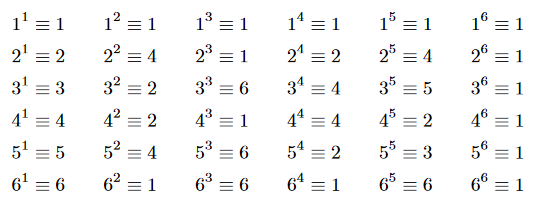
\includegraphics[width=1\textwidth]{images/6.png}
\end{center}

\noindent Si può vedere che la colonna di destra, quella degli $a^{6}$, produce tutti $1$.

\section{Numero quadrato}

\begin{definition}
Sia \(p\) un numero primo dispari e sia $a \in Z^*_p$. Si dice che \(a\) è un residuo quadratico di modulo \(p\) se \(a\) è un quadrato modulo \(p\), ovvero esiste un numero \(c\) tale che \(c \equiv a \pmod p\). In caso contrario \(a\) è detto non residuo quadratico modulo \(p\).
\end{definition}

\noindent Dato $(G, *)$, un gruppo $G$ con l'operazione $*$, il numero di quadrati che contiene è esattamente uguale a $\frac{p-1}{2}$, ovvero a tutti e soli gli elementi $g^{2i}$ (elementi con esponente pari). Ogni elemento $g^{2i}$ ha due radici:
\begin{align*}
 	g^{2i}=
 	    \begin{cases}
 	   g^i \\ 
 	    g^{i+\frac{p-1}{2}} \hspace{1cm} \rightarrow (g^{i+\frac{p-1}{2}})^2 = g^{2i}\cdot g^{p-1} = g^{2i}\cdot 1
        \end{cases} 
\end{align*}

\noindent Poiché le due radici di un numero sono opposte, allora $g^{\frac{p-1}{2}} \equiv -1$. Quindi elevare un generatore alla cardinalità del gruppo dà l'unità, mentre elevarlo alla metà della cardinalità dà l'opposto dell'unità.

\paragraph{Quadrati in $Z_{pq}^*$} Dato $Z_{pq}^*$, con $p, q$ numeri primi, il numero di quadrati contenuto nell'insieme è $\frac{\varphi}{4}$, ovvero il numero di quadrati comuni a $Z_{p}^*$ e $Z_{q}^*$.

\noindent Dato $p$ numero primo, come è possibile capire se un dato numero $a$ sia uguale a un quadrato modulo $p$? Escludendo il risolvere il problema del logaritmo discreto per $a$ e verificare se il risultato è pari o dispari, un modo per farlo è verificare se $x_i^2 = a$, per ogni $x_i \in 0, 1, 2, 3, 4, ..., p-1$. Esistono modi più efficienti? 

\begin{definition}[Simbolo di Legendre]
Il simbolo di Legendre è definito come segue:
\begin{align*}
    \left( \frac{a}{p} \right) &= a^{\frac{p-1}{2}} \pmod p\\\\
    \left( \frac{a}{p} \right) &= 
    \begin{cases}
        1 & \text{ se } a \text{ è un residuo quadratico modulo } p\\
        -1 & \text{ se } a \text{ è un non residuo quadratico modulo } p\\
    \end{cases}
\end{align*}
\end{definition}

\noindent Infatti:
\begin{itemize}
    \item Sia $a = g^{2i}$, ovvero un quadrato, allora
\begin{align*}
    a^{\frac{p-1}{2}}= (g^{2i})^{\frac{p-1}{2}} = (g^i)^{(p-1)} = 1
\end{align*}
\item Sia $a = g^{2i+1}$, ovvero un non quadrato, allora
\begin{align*}
    a^{\frac{p-1}{2}}= (g^{2i+1})^{\frac{p-1}{2}} = (g^{2i})^{\frac{p-1}{2}} \cdot g^{\frac{p-1}{2}} = 1 \cdot (-1) = -1
\end{align*}
\end{itemize}

\noindent Il simbolo di Legendre ritorna $1$ se $a$ è un quadrato modulo $p$ o $-1$ se non lo è. 

Si può calcolare questo algoritmo in tempo polinomiale, con numeri da migliaia di bit? Il simbolo di Legendre consiste nel calcolare una potenza, che equivale nella pratica a calcolare una serie di moltiplicazioni. Quindi la domanda diventa: esiste un algoritmo per eseguire moltiplicazioni in tempo polinomiale? Si, il \textbf{Fast Power Algorithm}. 

Praticamente il simbolo di Legendre permette di ottenere il bit meno significativo del numero, che permette di capire immediatamente se il numero è pari (0) o dispari (1).\\

\noindent Dato $n=pq$, come è possibile capire se un numero $a$ è un quadrato in $Z_n^*$? Il modo più semplice sarebbe fattorizzare $n$ in $p$ e $q$ e calcolare il simbolo si Legendre di $a$ rispetto ai due fattori. Poichè fattorizzare è difficile (non esistono algoritmi efficienti), allora anche determinare se $a \in Z_n^*$ dovrebbe essere difficile. In realtà non è proprio così. 

Il simbolo di Jacobi, una generalizzazione del simbolo di Legendre, permette di determinare $\left(\frac{a}{n} \right)$ senza dover fattorizzare.
\begin{definition}[Simbolo di Jacobi] Siano \(a\) e \(b\) due interi, con \(b\) dispari e positivo. Supponendo che la fattorizzazione di \(b\) in numeri primi sia 
\begin{align*}
    b = p_1^{e_1} \cdot p_2^{e_2} \cdot ... \cdot p_t^{e_t}
\end{align*}

\noindent allora il simbolo di Jacobi \(\left(\frac{a}{n}\right)\) è definito dalla formula 
\begin{align*}
    \left(\frac{a}{n}\right) = \left(\frac{a}{p_1}\right)^{e_1} \left(\frac{a}{p_2}\right)^{e_2} ... \left(\frac{a}{p_t}\right)^{e_t}
\end{align*}
\end{definition}

\noindent Il simbolo di Jacobi $\left(\frac{a}{n}\right)$ gode delle seguenti proprietà:
\begin{align*}
    \left(\frac{a}{n_1n_2}\right) = \left(\frac{a}{n_1}\right)\left(\frac{a}{n_1}\right)
\end{align*}
\begin{align*}
        \left(\frac{a_1a_2}{n}\right) = \left(\frac{a_1}{n}\right)\left(\frac{a_2}{n}\right)
\end{align*}

\noindent Se $n$ è un numero primo, allora il simbolo di Jacobi equivale al simbolo di Legendre. Se scompongo $n$ in numeri primi, allora ogni simbolo di Jacobi $\left(\frac{a}{p_i}\right)$ mi ritorna $1$ o $-1$:
\begin{align*}
    \left(\frac{a}{n}\right) &= \left(\frac{a}{pq}\right) = \left(\frac{a}{p}\right)\left(\frac{a}{q}\right)
\end{align*}

\noindent Il simbolo di Jacobi, come detto all'inizio, è risolvibile con un algoritmo polinomiale che non richiede la scomposizione in fattori primi.

Tornando al caso iniziale $n = pq$, nel calcolo del simbolo di Jacobi $\left(\frac{a}{pq}\right)$ si possono incontrare tre casi:
\begin{enumerate}
    \item $a$ è un quadrato sia in $Z_p^*$ che in $Z_q^*$ (probabilità $\frac{1}{4}$):
        \begin{align*}
            \left(\frac{a}{pq}\right) = \left(\frac{a}{p}\right)\left(\frac{a}{q}\right) = 1 \cdot 1 = 1
        \end{align*}
    \item $a$ è un quadrato sia in $Z_p^*$ ma non $Z_q^*$ (probabilità $\frac{1}{4}$) o viceversa (probabilità $\frac{1}{4}$):
        \begin{align*}
            \left(\frac{a}{pq}\right) = \left(\frac{a}{p}\right)\left(\frac{a}{q}\right) = 1 \cdot (-1) = -1\\\\
            \left(\frac{a}{pq}\right) = \left(\frac{a}{p}\right)\left(\frac{a}{q}\right) = (-1) \cdot 1 = -1
        \end{align*}
    \item $a$ non è un quadrato sia in $Z_p^*$ ne in $Z_q^*$ (probabilità $\frac{1}{4}$):
        \begin{align*}
            \left(\frac{a}{pq}\right) = \left(\frac{a}{p}\right)\left(\frac{a}{q}\right) = (-1) \cdot (-1) = 1
        \end{align*}
\end{enumerate}

\noindent Dai tre casi sopra, si può capire che il simbolo di Jacobi è limitato rispetto al simbolo di Legendre, in quanto è in grado solamente di decidere se un numero è un non quadrato nel caso particolare in cui è un quadrato in $Z_p^*$ e non quadrato in $Z_q^*$ (o viceversa).
Il simbolo di Jacobi si può quindi riassumere così:
\begin{align*}
    \left(\frac{a}{n}\right)=
 	    \begin{cases}
 	   -1& \mbox{ $a$ è un non quadrato}\\ 
 	    1& \mbox{ non so}
        \end{cases} 
\end{align*}

\noindent Di conseguenza, determinare se dato un numero con simbolo di Jacobi $1$ è quadrato o non quadrato è un problema difficile.

\section{Fast Powering Algorithm}
In molti crittosistemi come RSA e DH, i due attori necessiteranno di calcolare potenze di grandi dimensioni. Un modo per calcolare ad esempio $a^b \pmod n$ è per moltiplicazioni ripetute di $a$. Quindi
\begin{align*}
    a_1 \equiv a \pmod n \hspace{1cm} a_2 \equiv a_1 \cdot a \pmod n \hspace{1cm} ... \hspace{1cm} a_{b} \equiv a_{b-1} \cdot a \pmod n
\end{align*}

\noindent Se $b$ è un numero elevato, l'algoritmo non è pratico. Un modo migliore per calcolare la potenza è usare l'espansione binaria di $b$ per convertire il calcolo in una successione di quadrati e moltiplicazioni.\\
 
\noindent Ad esempio, dato $b = 75 = 1001011$, le rispettive potenze saranno:
 \begin{align*}
     2^6+2^3+2^1+2^0 
 \end{align*}
 \noindent Quindi:
 \begin{align*}
     a^b = a^{2^6+2^3+2^1+2^0} = a^{2^6} *a^{2^3}*a^{2^1}*a^{2^0}
 \end{align*}

\noindent Questa sequenza di valori è semplice da calcolare in quanto ogni numero nella sequenza è il quadrato del precedente:
\begin{align*}
    a^{2^0} &= a\\
    a^{2^1} &= a*a\\
    a^{2^2} &= a^{{2^1}^2}
\end{align*}

\noindent Questo metodo è chiamato \textbf{iterative squaring} e permette di calcolare le potenze in un numero di moltiplicazioni proporzionale ai bit di $b$. Calcola via via le potenze di $a$, elevate a potenze di 2, e verifica a vedere se il corrispondente bit dell'espressione binaria di $b$ vale $0$ o $1$: se vale $0$ non fa nulla, se vale $1$ moltiplica il risultato parziale per la potenze che ha calcolato.

\begin{algorithm}[H]
\caption{Iterative squaring EXP(a, b)}\label{alg:cap}
\begin{algorithmic}
\State $y \gets 1$
\State $t \gets a$
\While{$b \neq 0$}
\If{$b \% 2 == 1$}
    \State $y \gets y \times t$
\EndIf
    \State $b \gets b / 2$
    \State $t \gets t \times t$
\EndWhile
\end{algorithmic}
\end{algorithm}

\noindent Complessità dell'algoritmo, in funzione dei bit di $a$ e $b$:

\begin{algorithm}[H]
\caption{Iterative squaring EXP(a, b) - complessità}\label{alg:cap}
\begin{algorithmic}
\State $y \gets 1$ \Comment{lineare nel numero di bit di b}
\State $t \gets a$ \Comment{lineare, devo copiare tutti i bit di a}
\While{$b \neq 0$} \Comment{lineare}
\If{$b \% 2 == 1$} \Comment{costante, guardo il bit meno significativo }
    \State $y \gets y \times t$ \Comment{quadratico nella lunghezza del numero}
\EndIf
    \State $b \gets b / 2$ \Comment{lineare o costante in base a come salvo il numero}
    \State $t \gets t \times t$ \Comment{quadratico}
\EndWhile
\end{algorithmic}
\end{algorithm}

\noindent L'algoritmo è quindi di complessità cubica, con il corpo del while è quadratico ripetuto per ogni bit di $b$, quindi l'algoritmo è cubico. Questo però non è corretto. Se ad esempio moltiplichiamo  $100*100$, il risultato avrà quattro 0. Se moltiplichiamo il risultato ancora per $100$, il numero di 0 finali diventeranno sei. Quindi in realtà la complessità sarebbe esponenziale, ovvero $2^k$. Come possiamo riportare l'algoritmo a complessità cubica? Basta aggiungere dei modulo $n$ nei calcoli intermedi:

\begin{algorithm}[H]
\caption{Iterative squaring EXP(a, b) ottimizzato}\label{alg:cap}
\begin{algorithmic}
\State $y \gets 1$
\State $t \gets a$
\While{$b \neq 0$}
\If{$b \% 2 == 1$}
    \State $y \gets (y \times t) \% n$
\EndIf
    \State $b \gets b / 2$
    \State $t \gets (t \times t) \% n$ 
\EndWhile
\end{algorithmic}
\end{algorithm}

\section{Introdurre casualità}

Se moltiplico un quadrato per un non quadrato con $J=1$ ottengo un non quadrato con $J=1$; se moltiplico due non quadrati con $J=1$ ottengo un quadrato. In generale:
\begin{itemize}
    \item Se ho un oggetto e lo moltiplico per un quadrato mantengo la quadraticità;
    \item Se ho un oggetto e lo moltiplico per un non quadrato ne inverto la quadraticità.
\end{itemize}

\noindent Dato $a \in Z_n^*$ con $\left(\frac{a}{n}\right) = 1$, vogliamo ottenere un oggetto con la stessa quadraticità di $a$, ma distribuito uniformemente tra gli oggetti con la stessa quadraticità. Si può fare così:
\begin{align*}
    &\text{Sia } x \in_R Z_n^* \hspace{2cm} (\in_R == \text{ l'elemento viene preso uniformemente dall'insieme})\\
    &\text{Ret } x^2 \cdot a
\end{align*}

\section{Problemi difficili}
Un problema si definisce difficile se non esiste un algoritmo efficiente (che funziona in quello che chiamiamo tempo polinomiale) che è in grado di risolverlo. Spesso non si sa se esiste un metodo per risolvere questi problemi difficili in modo efficiente, ma solo che attualmente non si conosce un modo per farlo. Tuttavia, la maggior parte dei problemi difficili utilizzati nella crittografia moderna sono stati ampiamente studiati e quindi si ha fiducia che l'ipotesi di difficoltà sia valida.

\subsection{Problema del logaritmo discreto}
Sia $p$ un numero primo di grandi dimensioni. Allora esiste un generatore $g$ tale per cui ogni elemento diverso da zero appartenente a $Z_p^*$ è uguale  a qualche potenza di $g$. Per il \textit{Fermat’s little theorem} $g^{p-1} = 1$ e non esiste alcuna potenza positiva di $g$ più piccola che è uguale a $1$. In modo equivalente, la lista di elementi
\begin{align*}
    1, \ g, \ g^2, \ g^3, \ ... \ , \ g^{p-1}
\end{align*}
\noindent è una lista completa degli elementi di $Z_p^*$.

\begin{definition}
Sia \(g\) un generatore di $Z_p^*$ e sia $h$ un elemento non zero appartenente all'insieme. Il probema del logaritmo discreto $DLG$ è il problema di trovare un esponente $x$ tale per cui
\begin{align*}
    g^x \equiv h \pmod p
\end{align*}

\noindent Il numero $x$ è chiamato logaritmo discreto di $h$ per la base $g$.
\end{definition}

\noindent Tuttavia, se c'è una soluzione, allora ce ne sono infinite, perché il piccolo teorema di Fermat dice che $g^{(p-1)} \equiv 1 \pmod p$. Quindi se $x$ è una soluzione di $g^x = h$, allora anche $x + k(p - 1)$ è una soluzione per ogni valore di $k$, perché
\begin{align*}
    g^{x+k(p-1)} = g^x \cdot (g^{p-1})^k \equiv h \cdot 1^k \equiv h \pmod p
\end{align*}

\noindent A volte, per concretezza, ci riferiamo al “logaritmo discreto” come all'intero $x$ compreso tra $0$ e $p - 2$ che soddisfa la congruenza $g^x \equiv h \pmod p$.

\subsection{Problema delle radici quadrate modulo $pq$ / residuo quadratico}
Sappiamo che la fattorizzazione di un numero e il logaritmo discreto di un numero sono due problemi difficili. Vogliamo ora dimostrare che il calcolare delle radici quadrate di un numero in modulo $pq$ non è più semplice di fattorizzare.
\begin{lemma}
Siano $x, y$ due radici del quadrato $a \in Z_n^*$ con $x \ne$ $\pm y \pmod n$. Allora $MCD(x+y, n)$ è $p$ o $q$.
\end{lemma}

\begin{proof}
\begin{align*}
    &x^2 \equiv y^2\\
    &x^2 - y^2 = 0\\
    &(x+y)(x-y) = 0\\
    &(x+y)(x-y) = kn \hspace{1cm} \text{il resto della divisione per $n$ è 0, quindi il prodotto è un multiplo di $n$}
\end{align*}
\noindent Si presentano tre casi:
\begin{itemize}
    \item Supponendo che $p \mid(x+y)$, è possibile che $q \mid(x+y)$? Se è vero allora $n = pq$ divide $(x+y)$. Allora $(x+y)$ deve essere un multiplo di $n$. $(x+y) \equiv 0 \pmod n$ e quindi $x = -y \pmod n$ (per definizione di congruenza modulo $n$). IMPOSSIBILE.

   \item Supponendo $q \mid(x+y)$, è possibile che $p \mid(x+y)$? IMPOSSIBILE.

   \item  Infine, è possibile $p \nmid(x+y)$ e $q \nmid(x+y)$? $p$ e $q$ sono fattori del prodotto $(x+y)(x-y)$ e quindi devono essere fattori di almeno uno dei due oggetti. Se nessuno dei due è divisore di $(x+y)$, allora devono essere divisori di $(x-y)$, ma allora $x \equiv y$. IMPOSSIBILE.
\end{itemize}
\end{proof}

\noindent Supponiamo che esista un algoritmo $A \in PPT$ (Probabilistic Polinomial Time) in grado di calcolare la radice quadrata di un numero:

\begin{algorithm}[H]
\caption{Algoritmo di fattorizzazione FATTORIZZA(n)}\label{alg:cap}
\begin{algorithmic}
\State $x \in_R Z_n^*$
\State $y \gets A(x^2)$
\State $z \gets MCD(x+y, n)$
\If{$z \ne n$}
    \State \Return $n$
\Else
    \State \Return FATTORIZZA(n)
\EndIf
\end{algorithmic}
\end{algorithm}

\noindent FATTORIZZA prende un quadrato a caso $x^2$, di cui conosce una radice $x$ (presa uniformamene tra le sue quattro radici). Il quadrato viene quindi passato all'algoritmo $A$, che restituisce un'altra radice quadrata, scelta in qualche modo diverso da come vene scelto $x$. Qual è la probabilità che $A$ ritorni la radice iniziale presa o il suo opposto? $1 / 2$. Quindi sempre con probabilità $1 / 2$ l'algoritmo $A$ ritornerà le radici $\pm y$. 

La probabilità con cui l'algoritmo ritorna la radice giusta è $1 / 2$. Come si può portare la probabilità a $1$? Basta ripetere il test un  numero di volte. Ad esempio, riprovando una seconda volta la probabilità di fallire diventa $\frac{1}{4}$, alla terza $\frac{1}{8}$ e così via (distribuzione geometrica). 

Supponendo che un attaccante disponga di un algoritmo $A$ in grado di calcolare le radici di un quadrato, allora sarà in grado anche di fattorizzare un numero. Di conseguenza il problema delle radici in modulo $pq$ è dimostrabile sicuro. Infatti risolvere questo problema equivale a risolvere il problema di fattorizzare.

\section{Altro}

\paragraph{Problema del logaritmo discreto $DL(a, g)$} Dato il gruppo $Z^*_p$, un suo generatore $g$ e un elemento $a\in Z^*_p$, allora esisterà una potenza $i$ del generatore tale per cui:
\begin{align*}
    g^i \equiv g^{i + k(p-1)} = a
\end{align*}

\noindent visto che le varie potenze del generatore enumerano l'intero gruppo. Dato $g$ e $g^i$, trovare $i$ è molto difficile. Questo problema è detto problema del logaritmo discreto (discreto in quanto lavoro su un insieme finito) e ad oggi non esistono algoritmi efficienti per risolverlo.

\paragraph{One way function} Una funzione facile da calcolare ma difficile da invertire è detta one-way function. Un esempio di funzione di questo tipo è quella del logaritmo discreto: è semplice calcolare $g^i$, ma è difficile calcolare $i$ da $g^i$.

\paragraph{Come scegliere casualmente un numero primo di $k$ bit} L'uso della casualità permette di risolvere molti problemi che normalmente non saremmo in grado di risolvere. Per scegliere casualmente un numero primo, sparo un sequenza di $k$ bit a caso. Esiste un teorema sulla densità dei numeri primi nei naturali tale per cui questa è proporzionale al numero di bit usati per rappresentare il numero. Dati $k$ bit, per questo teorema $1 \backslash k$ volte ottengo un numero primo. Quindi mi servono in media $k$ tentativi casuali per generarlo. 

\paragraph{Test di primalità di un numero} Esistono più algoritmi per verificare se un numero è primo. Ad oggi il migliore funziona come segue: esiste un test che è possibile fare usando un numero e un numero più piccolo. Questo test disce si o no. Se dice si, il numero è composto; se dice no, non sa se il numero è composto (per quel numero è primo). Metà dei numeri più piccoli di $n$ sono tesimoni del fatto che un numero non sia primo. Quindi prendo un numero più piccolo del numero che ho generato e faccio il test. Se il test mi dice si, il numero non è primo; se mi dice no riprovo con un numero più piccolo. Eseguo il test per $x$ volte. Se tutte le volte mi dice che è primo allora lo accetto come primo. La probabilità di accettare un numero che non è primo è $\frac{1}{2^x}$.

\chapter{Crittografia a chiave pubblica}
\label{chapter4}

La crittografia a chiave pubblica prevede l'uso di due chiavi: $P_k$ (Public key) e $S_k$ (Secret Key). La chiave privata è posseduto da un solo agente; la chiave pubblica è posseduta da tutti. La $P_k$ è usata per codificare il messaggio; la $S_k$ è usata per decodificarlo. Senza $S_k$ non deve essere possibile ricavare il plaintext dal cyphertext. Con questo sistema chiunque può codificare messaggi, ma solo che possiede la secret key può leggerli.\\

\noindent Componenti del sistema:
\begin{align*}
    G: \ &1^K \rightarrow (P_k, S_k)\\
    E: \ &(m, P_k) \rightarrow E(m, P_k)\\
    D: \ &(c, S_k) \rightarrow D(c, S_k)
\end{align*}

\noindent In questo sistema vale sempre:
\begin{align*}
   \forall m \ D(E(m, P_k), S_k) = m
\end{align*}

\noindent L'input $1^k$ del generatore $G$ è il security parameter, che in questo caso rappresenta la lunghezza, in bit, della chiave. Non sempre rappresenta la lunghezza della chiave; in generale il security parameter è quel numero/parametro tale per cui al suo crescere il protocollo diventa sempre più sicuro.

\section{Scambio di chiavi Diffie-Hellman}

L'algoritmo di scambio di chiavi Diffie-Hellman nasce per risolvere il seguente problema: Alice e Bob vogliono condividere una chiave segreta da utilizzare in una cifratura simmetrico, ma il loro unico mezzo di comunicazione è insicuro.

Per prima cosa Alice e Bob concordano su un numero primo $p$ e un generatore $g$ di $Z_p^*$, che rendono pubblici. 
A questo punto Alice sceglie un intero $x$ che terrà segreto e Bob un intero $y$ che terrà anch'egli segreto. Bob e Alice usano i loro numeri interi segreti per calcolare
\begin{align*}
     	\underbrace{g^x \pmod{p}}_{Alice} \hspace{1cm}\text{e}\hspace{1cm} \underbrace{g^y \pmod{p}}_{Bob}
\end{align*}
\noindent Il passo successivo consiste nello scambiare, sul canale non sicuro, i due risultati: Alice invia $g^x$ a Bob e Bob invia $g^y$ a Alice. Infine Alice e bob utilizzano i rispettivi interi segreti per calcolare
\begin{align*}
     	\underbrace{(g^y)^x \pmod{p} = g^{yx} \pmod{p}}_{Alice} \hspace{1cm}\text{e}\hspace{1cm} \underbrace{(g^x)^y \pmod{p} = g^{xy} \pmod{p}}_{Bob}
\end{align*}
\noindent I due valori calcolati sono gli stessi.\\

\noindent Supponendo che un attaccante ascolti l'intera conversazione, egli potrà ricostruire la chiave segreta condivisa $g^x^y$ solo se riuscirà a trovare $x$ tale per cui $g^x \pmod p$ equivale al valore inviato da Alice sul canale. Stesso discorso per $y$. Le linee guida attuali suggeriscono che Alice e Bob scelgano un $p$ primo avente circa 1000 bit.

L'attaccante conosce $g^a \pmod{p}$ e $g^b \pmod{p}$, ma anche $g$ e $p$. Quindi se riuscisse a estrarre uno solo degli esponenti $a$ e $b$ da $g^a \pmod{p}$ e $g^b \pmod{p}$, allora sarebbe in grado di calcolare la chiave di sessione $g^a^b$. Potrebbe sembrare che Alice e Bob siano al sicuro a condizione che l'attaccante non sia in grado di risolvere il Problema del Logaritmo Discreto (DLP), ma questo non è del tutto corretto. È vero che un metodo per trovare il valore condiviso di Alice e Bob è risolvere il DLP, ma non è questo il problema preciso che l'attaccante deve risolvere. La sicurezza della chiave condivisa di Alice e Bob si basa sulla difficoltà del seguente problema, potenzialmente più semplice.

\begin{definition}
Sia \(p\) un numero primo e \(g\) un generatore di \(Z_p^*\). Il problema di Diffie-Hellman (DHP) è il problema di calcolare il valore \(g^a^b \pmod p\) a partire dai valori conosciuto \(g^a \pmod p\) e \(g^b \pmod p\).
\end{definition}

\noindent È chiaro che il DHP non è più difficile del DLP. Se l'attaccante riesce a risolvere il DLP, allora può calcolare gli esponenti segreti di Alice e Bob. Ma il viceversa è meno chiaro. Supponiamo che l'attaccante abbia un algoritmo che risolva efficientemente il DHP. Può usarlo anche per risolvere in modo efficiente il DLP? La risposta ad oggi non è nota, e quindi DF non è dimostrabilmente sicuro (non si è in grado di dimostrare che rompere DH è tanto difficile quando risolvere il DLP).\\

\subsection{Ipotesi di Diffie-Hellman}
DH non è dimostrabilmente sicuro secondo i problemi difficili per ora trovati. D'altro canto però, qualcuno potrebbe costruire degli algoritmi con alla base di DH. In questi casi tali algoritmi si dimostrano sicuri sotto l'ipotesi che DH sia sicuro. Per fare ciò nasce l'ipotesi di DH.

Supponiamo che sia difficile distinguere una tripla $(g^x, g^y, g^x^y)$, con $x, y \in \{1, ..., p-1\}$, da una tripla $(g^x, g^y, g^z)$, con $x, y \in \{1, ..., p-1\}$\footnote{Praticamente se do la soluzione all'attaccante lui non riesce a capire che è la soluzione.}. Se l'attaccante identifica $x$, allora riesce a riconoscere la tripla corretta. In caso contrario, ha una possibilità su due di indovinare la tripla corretta. Infatti, essendo la probabilità di indovinare $x$ $Pr=\frac{1}{2^k}$, con $k$ i bit della chiave, allora probabilità totale di indovinare la tripla è:
\begin{align*}
    Pr = \frac{1}{2^k} + \frac{1}{2} (1 - \frac{1}{2^k}) = \frac{1}{2} + \frac{1}{2^{k+1}}
\end{align*}
\noindent L'idea è che anche se un attaccante dispone di un algoritmo per indovinare la tripla giusta, questo gli porta un vantaggio molto minimale rispetto allo sparare a caso.

\section{Crittosistema di Rivest, Shamir e Adleman (RSA)}

\noindent RSA si basa sulla seguente dicotomia:
\begin{itemize}
    \item \textbf{Setup:} Siano $p, q$ due numeri primi di $k/2$ bit ognuno (comunque di grandi dimensioni) e siano $e, c$ due interi;
    \item \textbf{Problema:} Risolvere la congruenza $x^e \equiv c \pmod{pq}$ per la variabile $x$;
    \item \textbf{Facile:} Bob, che conosce i valori di $p$ e $q$, può trovare facilmente $x$ (teoremi sopra);
    \item \textbf{Difficile:} Un attaccante, che non conosce i valori dei due primi, non può calcolare facilmente $x$;
    \item \textbf{Dicotomia:} Risolvere $x^e \equiv c \pmod{pq}$ è facile per chi conosce specifiche informazioni aggiuntive (ovvero i valori di $p$ e $q$), ma è difficile per chiunque altro.
\end{itemize}

\noindent La chiave segreta di Bob è una coppia di grandi primi $p,q$. La sua chiave pubblica è la coppia $(n, e)$ costituita dal prodotto $n= pq$ e da un esponente $e$ che è relativamente primo a $(p - 1)(q - 1)$. Alice prende il suo testo in chiaro e lo converte in un intero $m$ compreso tra $1$ e $n$. Crittografa $m$ calcolando
\begin{align*}
    c \equiv m^e \pmod n
\end{align*}

\noindent L'intero $c$ è il suo testo cifrato, che invia a Bob. È quindi semplice per Bob risolvere la congruenza $x^e \equiv c \pmod n$ per recuperare il messaggio di Alice $m$, perché Bob conosce la fattorizzazione $n = pq$. Un attaccante, d'altra parte, può intercettare il testo cifrato $c$, ma a meno che non sappia come fattorizzare $n$, presumibilmente avrà difficoltà a risolvere $x^e \equiv c \pmod n$.

\subsection{Generazione delle chiavi, encryption e decryption}

\textbf{Generazione chiavi}
\noindent \textbf{Output:} chiave pubblica $(n, e)$ e chiave privata $(n, d)$.
\begin{enumerate}
    \item Scegli la grandezza del security parameter $k$.
    \item Scegli due numeri $p, q$ di $k/2$ bit ciascuno.
    \item Calcola $n = pq$.
    \item Calcola $\varphi(n) = (p-1)(q-1)$.
    \item Calcola l'esponente $e \in_R Z_{\varphi(n)}^*$ tale per cui
    \begin{align*}
        MCD(e, \varphi) = 1
    \end{align*}
    \item Calcola la chiave privata $d$ tale per cui
    \begin{align*}
        de \equiv 1 \pmod{\varphi(n)}
    \end{align*}
\end{enumerate}

\noindent \textbf{Encryption}
Data la chiave pubblica $(n, e)$ e il messaggio $m$, la funzione di encryption è
\begin{align*}
    c = m^e \pmod n
\end{align*}

\noindent \textbf{Encryption}
Data la chiave pubblica $(n, d)$ e il cyphertext $c$, la funzione di decryption è
\begin{align*}
    m = c^d \pmod n
\end{align*}

\noindent La condizione $MCD(e, \varphi(n)) = 1$ assicura che assicura che l'inverso $e \pmod{\varphi(n)}$ esista, in modo che ci sia sempre una chiave privata $d$.

\noindent L'essenza di RSA può essere rappresentata con la seguente equazione:
\begin{align*}
    (m^e)^d = m^{ed} = m^{1+ k\varphi(n)} = m^{k\varphi(k)} \cdot m = 1^k \cdot m = m \pmod n
 \end{align*}
 
\subsection{Problema delle radici quadrate (versione matematica)}
Se rimpiazziamo, nel \textit{Fermat’s little theorem}, il numero primo $p$ con un numero non primo $n$ vale ancora $a^{p-1}\equiv 1 \pmod p$? In generale no. Esiste però un caso particolare, quando $n = pq$ (con $p, q$ primi), che è il caso più importante per la crittografia. 
        
\begin{theorem}[Formula di Eulero per \(pq\)]
    Siano \(p, q\) due numeri primi distinti e sia $g = MCD(p-1, q-1)$. Allora
    \begin{align*}
        a^{(p-1)(q-1)/g} \equiv 1 \pmod {pq} \text{ per tutti gli $a$ che soddisfano MCD(a, pq)=1}
    \end{align*}
    \noindent In particolare, se $p$ e $q$ sono due numeri primi dispari, allora 
    \begin{align*}
        a^{(p-1)(q-1)/2} \equiv 1 \pmod {pq} \text{ per tutti gli $a$ che soddisfano MCD(a, pq)=1}
    \end{align*}
\end{theorem}

\noindent Lo scambio di chiavi di DH si affida alla difficoltà di risolvere equazioni nella forma 
\begin{align*}
    a^x \equiv b \pmod p
\end{align*} 
\noindent dove $a, b, p$ sono quantità note e $x$ è la variabile da trovare. RSA, invece, si affida alla difficoltà di risolvere equazioni nella forma
\begin{align*}
    x^e \equiv c \pmod n
\end{align*}
\noindent dove le quantità note sono $e, c, n$ e la $x$ è sconosciuta. IN altre parole, RSA si affida all'assunzione che è difficile prendere radici e-esime modulo $n$. 

Se $n$ è primo, risulta che è relativamente facile calcolare la radice esima in modulo $n$, come mostrato di seguito.

\begin{theorem}
    Sia \(p\) un numero primo e \(e \ge\) 1 un intero che soddisfa \(MCD(e, p-1)=1\). Allora \(e\) ha un inverso modulo \(p\), ovvero
    \begin{align*}
        de \equiv 1 \pmod{p-1}
    \end{align*}
    \noindent Quindi la congruenza 
    \begin{align*}
        x^e \equiv c \pmod p
    \end{align*}
    \noindent ha l'unica soluzione \(x \equiv c^d \pmod p\).
\end{theorem}

\noindent Il teorema sopra mostra che è facile prendere una radice e-esima se il modulo è un numero primo $p$. La situazione per un modulo complesso $n$ è simile, ma è semplice da calcolare solo se i fattori di $n$ sono conosciuti.

Vediamo ora il caso in cui $n = pq$ è il prodotto di due numeri primi.

\begin{theorem}
    Siano \(p, q\) due primi distinti e sia \(e \ge 1\) tale per cui \(MCD(e, (p-1)(q-1)) = 1\). Allora \(e\) ha un inverso modulo \((p-1)(q-1)\), ovvero
    \begin{align*}
        de \equiv 1 \pmod{(p-1)(q-1)}
    \end{align*}
    \noindent Quindi la congruenza 
    \begin{align*}
        x^e \equiv c \pmod{pq}
    \end{align*}
    \noindent ha l'unica soluzione \(x \equiv c^d \pmod{pq}\).
\end{theorem}

\subsection{Debolezze di RSA}
RSA ha diverse debolezze:
\begin{itemize}
    \item In passato è stato attaccato a causa di una sua errata implementazione. Il protocollo vuole che il valore $e$ venga scelto \textbf{casualmente} tra tutti i numeri relativamente primi in $\varphi_n$. Gli implementatori usavano però funzioni random a 64 bit per generare $e$ o $d$, andando a settare i bit "mancanti" a zero. Supponendo che il valore debba essere a 564 bit, il problema è che la probabilità di generare casualmente un numero con i primi 500 bit è estremamente bassa ($\frac{1}{2^{500}}$);
    \item Supponendo di lavorare in $Z_n^*$, se il messaggio cifrato $m^e$ è più piccolo di $n$, calcolare la radice e-esima (come visto sopra) è facile. Quindi scenari con messaggi piccoli sono problematici per RSA;
    \item Supponiamo che l'insieme dei possibili messaggi che Alce possa spedire a Bob sia piccolo. Allora un attaccante potrebbe semplicemente cifrare tutte le possibili combinazioni e confrontarle con cyphertext inviato da Alice per capire qual è il messaggio originario. Quindi messaggi sparsi sono problematici in RSA;
    \item Siamo sicuri che tutti i bit dell'inverso del cyphertext siano difficili da calcolare? Ad esempio, col simbolo di Legendre, è possibile ottenere il bit meno significativo del logaritmo discreto. Per poter dire che un sistema è sicuro non basta che dal cyphertext non si possa ottenere il plaintext, ma non deve essere possibile estrarre \textbf{alcuna informazione parziale}. Per RSA non è dimostrato;
    \item Dati due messaggi ripetuti inviati nella stessa "comunicazione", RSA genererà lo stesso cyphertext. 
\end{itemize}

\noindent RSA è sicuro perché ad oggi non si conosce un algoritmo probabilistico polinomiale per il calcolo della radice e-esima di un numero. Ma cosa vuol dire questo? Che non esiste esiste un algoritmo che ritorna la radice e-esima? Ma se allora esistesse un algoritmo che ritorna $\sqrt[e]{a}$ con probabilità $1 / 100$? In questo caso, cosa vuol dire con probabilità $1 / 100$? Che l'algoritmo, se reiterato sullo stesso numero, in media con $100$ tentativi ritorna il risultato corretto\footnote{Applichiamo l'algoritmo una prima volta, se fallisce lo riapplichiamo una seconda e così via finché non ritorna il risultato corretto.}, oppure che funziona correttamente solo su $1 / 100$ degli $a$ possibili? 

Quindi il fatto che l'algoritmo calcoli la radice e-esima di $a$ con probabilità $1/100$ può voler dire:
\begin{enumerate}
    \item Dato un $a$ a caso, la probabilità che l'algoritmo arrivi a calcolare la radice e-esima è $1/100$;
    \item Fissato $a$, la probabilità che l'algoritmo ritorni il risultato è $1/100$.
\end{enumerate}

\noindent Il "modo" di trasformare la probabilità da $1/100$ a $1$ descritta appena sopra funziona solo nel secondo caso. Quindi se fossimo nel primo scenario saremmo al sicuro? In realtà no, anche nel primo caso la probabilità può essere trasformata in $1$:

\begin{definition}
Dato $a \in Z_n^*$ fissato e scelto $R \in_R Z_n^*$, allora $aR^e$ è un numero distribuito uniformemente tra gli elementi di $Z_n^*$. 
\end{definition}
\begin{proof}
Essendo l'elevamento $R^e$ invertibile, in quanto $e$ è scelto in modo che la radice e-esima dia esattamente $R$, allora la funzione che mappa $R$ in $R^e$ è una funzione invertibile tra due insiemi che hanno la stessa cardinalità, e quindi biettiva. Un elemento scelto uniformemente in $Z_n^*$ viene mappato in un elemento scelto uniformemente in $Z_n^*$. Se prendiamo un elemento distribuito uniformemente in $Z_n^*$ e lo moltiplichiamo per $a$, otteniamo ancora un elemento distribuito uniformemente in $Z_n^*$, essendo anche la moltiplicazione una funzione invertibile. Quindi $aR^e$ è un elemento casuale di $Z_n^*$. 
\end{proof}

\noindent Siamo partiti da un elemento $a$ fissato e siamo riusciti a costruire un elemento casuale in $Z_n^*$. Se a questo elemento cerchiamo di applicare l'algoritmo, $1/100$ volte abbiamo la risposta. Quindi abbiamo resto l'algoritmo del primo caso indipendente dal numero fissato $a$. Dato il nuovo input, l'algoritmo calcolerà con $Pr = 1/100$ la radice $\sqrt[e]{aR^e}$. Da questo risultato riusciamo a ottenere la radice e-esima di $a$? Si, in quanto
\begin{align*}
    \sqrt[e]{aR^e} = R\sqrt[e]{a} = \frac{R\sqrt[e]{a}}{R} = \sqrt[e]{a}
\end{align*}

\noindent Siamo riusciti quindi a costruire un algoritmo che, a partire da una black-box con $a$ casuale calcola correttamente $ \sqrt[e]{a}$ con probabilità $1/100$, riesce a calcolare correttamente  $\sqrt[e]{a}$ con probabilità $1/100$ con $a$ fissato. 

Come verifichiamo che la radice ritornata sia quella corretta? Basta semplicemente prendere il risultato e elevarlo a $e$.

In generale, diciamo che un sistema è attaccabile quando il tempo necessario ad attaccarlo è polinomiale. Questo vuol dire che se esistesse un qualsiasi algoritmo in grado di calcolare $ \sqrt[e]{a}$ con probabilità polinomiale in $k$, noi saremmo in grado di trovare un algoritmo che calcola la stessa cosa con un tempo medio polinomiale in $k$. 
Poiché partiamo dall'idea che non esiste un algoritmo PPT in grado ci calcolare $ \sqrt[e]{a}$, non esiste nemmeno un algoritmo che riesce a calcolarla con una probabilità che sia polinomialmente piccola. La probabilità di successo di un eventuale algoritmo è più piccola di qualsiasi polinomio, dove per polinomio si intende
\begin{align*}
    \forall c : Pr[correttezza] < \frac{1}{k^c}
\end{align*}
\noindent Questa formula non è del tutto corretta, in quanto, solitamente, con chiavi piccole i protocolli sono attaccabili. La forma corretta è la seguente
\begin{align*}
    \exists c \ \forall \bar{k} \ \exists k > \bar{k} \ \big|Pr[attacco\_ha\_successo]\big| < k^{-c}
\end{align*}

\noindent Fissato un livello di difficoltà $c$, vogliamo che la probabilità di successo di un attaccante sia più piccola del polinomio costruito col quel livello di difficoltà $k^{-c}$. Non abbiamo però garanzia che questo sia sempre vero, ma se fissiamo una chiave sufficientemente lunga $\bar{k}$, allora possiamo rendere la probabilità di attacco inferiore al polinomio $k^{-c}$. Secondo questa definizione, idealmente aumentando la dimensione della chiave l'attacco diventa più difficile.\\

\noindent Dato $n$, è vero che non esiste un algoritmo PPT in grado di calcolare $\sqrt[e]{a}$? Esiste, ed è quello che conosce la fattorizzazione di $n$. Se fissiamo $n$, l'algoritmo che calcola $\sqrt[e]{a}$ esiste ed è quello che conosce l'informazione \textbf{trapdoor}, ovvero la fattorizzazione di $n$.

Quando diciamo che una funzione è difficile da calcolare dobbiamo essere precisi, dobbiamo dire input e output della funzione. Per RSA si pensa che non esista un algoritmo PPT che dati $n, e, a$ calcola $\sqrt[e]{a}$ in $Z_n^*$.

\subsection{Complessità di RSA}
Da un punto di vista computazionale, quanto è complesso RSA? Quanti passi di computazione dobbiamo fare con una chiave di $k$ bit? La complessità di $m^e$ è polinomiale: sommare due numeri a $k$ bit costa $k$, moltiplicarli costa $k^2$, elevarli tra loro costa $k^3$ (grazie all'iterative squaring). Quindi codifica e decodifica di RSA costano $k^3$. Se lavoriamo con $1'000$ bit, allora queste operazioni ci costano un miliardo di operazioni.

Diversamente AES ha un costo di codifica sul singolo blocco che è costante, in quanto alla fine lavora su tabelle e registri. Per questo motivo la crittografia a chiave pubblica non è generalmente usata per cifrare i messaggi, ma per cifrare e scambiare una chiave di sessione usata poi in codifiche simmetriche, molto meno costose.  

Diversamente da RSA, che permette di inviare una chiavi qualsiasi, Diffie-Hellman permette di scambiare un'unica chiave, sempre che non si crei una nuova chiave di DH ogni volta. 

\chapter{Crittografia a blocchi}
\label{chapter5}

I protocolli visti fin'ora permettono di codificare messaggi di dimensioni precise (per RSA dipende dalla dimensione della chiave). Se però dovessimo inviare un messaggio che supera queste dimensioni? Dato un messaggio di $n$ bit, con $n > k$, possiamo suddividere il messaggio in una serie di blocchi $m = m_1 \ m_2 \ ... \ m_l$, di $k$ bit ciascuno, cifrare ciascun blocco e inviare la sequenza di questi blocchi cifrati. 

La crittografia a blocchi (block cypher) differisce da quella  a flusso (stream cypher), che cifra il messaggio bit a bit man mano che viene reso disponibile.

Esistono più tecniche per cifrare i blocchi.

\section{Electronic Code Book (ECB)}

ECB è il metodo più semplice per cifrare un messaggio diviso in blocchi: codifichiamo separatamente ciascun blocco con la chiave $k$ e il crittosistema $E$ e poi ricostruiamo la sequenza in ordine.

\begin{center}
    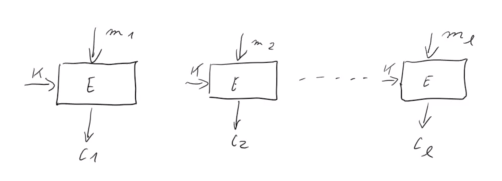
\includegraphics[width=1\textwidth]{images/ECB.png}
\end{center}

\noindent Questo sistema ha molte debolezze:
\begin{itemize}
    \item Blocchi che si ripetono producono lo stesso cyphertext, quindi sono riconoscibili;
    \item L'ordine dei blocchi, se scambiato, può generare messaggi ancora sensati. Noi possiamo ad esempio invertire i blocchi 2 e 7 e ottenere una manipolazione nota del plaintext pur non conoscendo il plaintext lavorando direttamente sul cyphertext (\textbf{malleabilità});
    \item È possibile fare un collage di blocchi provenienti da messaggi diversi ("Paga 100 euro a" -> "paga 10000 euro a").
\end{itemize}

\noindent L'unico vantaggio che ha è la possibilità di parallelizzare il lavoro. 

\section{Counter (CTR)}
CTR prevede di prendere di codificare un counter $ctr$ con il crittosistema $E$ e la chiave $k$, e mettere in XOR il risultato col blocco del messaggio da cifrare. Ad ogni cifratura, il counter viene incrementato di $1$. Il cyphertext finale è dato dalla ricomposizione dei risultati per ciascun blocco. 

\begin{center}
    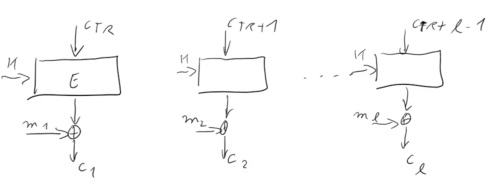
\includegraphics[width=1\textwidth]{images/CTR.png}
\end{center}

\noindent Con questo schema blocchi ripetuto generano cyphertext differenti e non è possibile fare collage di blocchi provenienti da messaggi differenti, a patto che il contatore sia differente. La debolezza di questo schema è il contatore: mittente e destinatario devono condividere il contatore e tenerlo sincronizzato. 

\section{Cypher Block Chaining (CBC)}
In CBC codifichiamo i blocchi del messaggio con il crittosistema $E$ e la chiave $k$ e, in ogni blocco successivo al primo, mettiamo in XOR il blocco con il cyphertext del blocco che lo precede. 

\begin{center}
    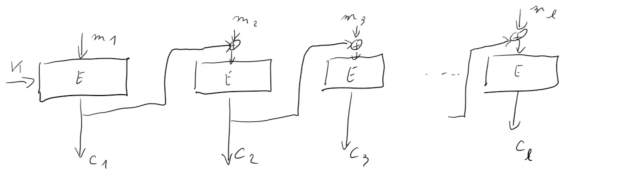
\includegraphics[width=1\textwidth]{images/CBC.png}
\end{center}

\noindent Il cyphertext del blocco precedente viene usato per modificare la sequenza di bit del blocco successivo. Con questo schema il collage non funziona e non esiste alcun contatore da mantenere condiviso. Il problema sta nel fatto che, se il cyphertext di un blocco contiene errori, questi vengono poi propagati in tutti i blocchi che lo seguono (es: in seguito ad errori di trasmissione).

Soffre inoltre del problema dei messaggi ripetuti. Questo problema può essere risolto aggiungendo un blocco casuale all'inizio del messaggio.

Vogliamo quindi trovare un sistema per evitare che l'errore di trasmissione si propaghi agli altri blocchi. Infatti qui, ad esempio, il blocco 

\section{Cypher Feedback}
Variazione del CBC che permette di trasmettere messaggi codificati bit per bit, piuttosto che blocco per blocco. Infatti in CBC il blocco $c_2$, ad esempio, non può essere inviato finché non abbiamo ottenuto completamente il blocco $m_2$.

\begin{center}
    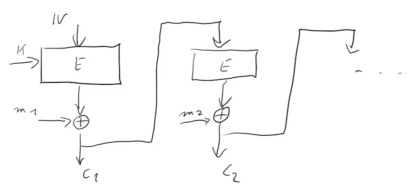
\includegraphics[width=0.7\textwidth]{images/CF.png}
\end{center}

\noindent Questo sistema utilizza un Initialization Vector $IV$ (da concordare con la controparte) che viene codificato con il crittosistema $E$ e la chiave $k$. Il risultato viene messo in XOR con il blocco da cifrare. Il risultato di questo viene usato sia come cyphertext del blocco corrente sia come nuovo $IV$ per la codifica del blocco successivo.

Il vantaggio di questo schema è che possiamo inviare il risultato dello XOR col blocco alla codifica del successivo bit a bit mentre viene generato. Lo schema che abbiamo costruito è a blocchi ma permette di fare la trasmissione a stream. Non è resistente ad errori di trasmissione. 

\section{Output Feedback}
In questo caso, diversamente da Cypher Feedback, inviamo alla codifica del blocco successivo l'output del crittosistema $E$, e non il risultato dello XOR.

\begin{center}
    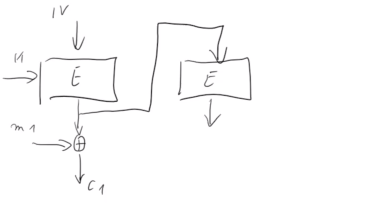
\includegraphics[width=0.7\textwidth]{images/OF.png}
\end{center}

\noindent Con questo scema un errore di trasmissione non ha influenza nel blocco successivo. Infatti, conoscendo l'$IV$, siamo in grado di calcolare tutte le uscite di ogni blocco senza dover leggere i cyphertext dei blocchi precedenti. Praticamente in ogni blocco usiamo una codifica della codifica di $IV$.
\chapter{Codifica di un singolo bit e di sequenze di bit}
\label{chapter6}

Supponiamo che Alice voglia usare un crittosistema a chiave pubblica per inviare a Bob 1 bit di informazione. A prima vista questa disposizione può sembrare intrinsecamente non sicura, in quanto tutto quello che deve fare un attaccante è cifrare i due possibili plaintext $m = 1$ e $m = 0$ e confrontarli con il cyphertext inviato da Alice. In generale, in ogni crittosistema in cui il pool di possibili messaggi è piccolo, tutto quello che deve fare un attaccante è cifrare tutte le possibilità e confrontarle con cyphertext inviato. 

\section{Crittosistema di Goldwasser-Micali}
La \textbf{cifratura probabilistica} è stata inventata da Goldwasser e Micali per aggirare questo problema. L'idea è che Alice scelga un plaintext $m$ e una stringa casuale di dati $r$ che andrà a cifrare con la chiave pubblica di Bob. Idealmente, poiché $r$ potrebbe variare su tutti i suoi possibili valori, il cyphertext $(m, r)$ varierà casualmente su tutti i possibili cyphertext generabili. Più precisamente, per ogni $m_1, m_2$ fissati e per un $r$ variabile, i cyphertext $E(m_1, r)$ e $E(m2, r)$ dovrebbero essere indistinguibili. Ovviamente per Bob non è necessario recuperare l'intero messaggio $(m, r)$ ma solamente $m$, quando decodifica.

A partire da questa idea, Goldwasser e Micali hanno creato un schema che, sebbene impratico in quando codifica un bit per volta, è semplice da descrivere e analizzare. Lo scema si basa sulla difficoltà del seguente problema:

\begin{definition}[Problema del residuo quadratico]
Siano \(p, q\) due numeri primi segreti di $k/2$ bit ciascuno e sia \(n = pq\) pubblico. Per un dato numero \(a\), determinare se \(a\) è un quadrato modulo \(n\), ovvero determinare se esiste un intero \(x\) tale per cui \(x^2 \equiv a \pmod n\).
\end{definition}

\noindent Bob, che conosce la fattorizzazione di $n$, può risolvere il problema molto facilmente in quanto 
\begin{align*}
    a \text{ è un quadrato modulo } p \Longleftrightarrow \left( \frac{a}{p}\right) = 1 \land \left( \frac{a}{q}\right) = 1 
\end{align*}

\noindent Un attaccante invece ha molta più difficoltà in quanto conosce solo il valore $n$. Il massimo che può fare è calcolare $\left(\frac{a}{n}\right)$, ma questo non dice se $a$ è un quadrato modulo $n$.

\subsection{Generazione delle chiavi, encryption e decryption}

\textbf{Generazione chiavi}
\noindent Bob sceglie:
\begin{itemize}
    \item $p, q$ primi segreti  di $k/2$ bit.
    \item $y \in_R Z_n^*$ \underline{non quadrato} con $(\frac{a}{p}) = (\frac{a}{q}) = 1$.
    \item Pubblica $n = pq$ e $y$.
\end{itemize}

\noindent \textbf{Encryption}
\noindent Alice:
\begin{itemize}
    \item Sceglie $m \in \{0, 1\}$.
    \item Sceglie $r \in_R Z_n^*$.
    \item Usa la chiave pubblica $(n, y)$ per calcolare:
    \begin{align*}
        c = \begin{cases}
                r^2 \pmod n & \text{ se } m=0\\
                yr^2 \pmod n & \text{ se } m=1
        \end{cases}
    \end{align*}
    \item Invia $c$ a Bob.
\end{itemize}

\noindent \textbf{Decryption}
\noindent Bob decifra il messaggio:
\begin{align*}
    m = \begin{cases}
                0 \pmod n & \text{ se } \left(\frac{c}{p} \right) = \left(\frac{c}{q} \right) = 1\\
                1 \pmod n & \text{ se } \left(\frac{c}{p} \right) = \left(\frac{c}{p} \right) = -1
        \end{cases}
\end{align*}

\noindent Il crittosistema di Goldwasser-Micali funziona come previsto in quanto:
\begin{align*}
    \left(\frac{c}{p} \right) = 
        \begin{cases}
                \left(\frac{r^2}{p} \right) = \left(\frac{r^2}{p} \right)^2 = 1 & \text{ se } m = 0\\
                \left(\frac{ar^2}{p} \right) = \left(\frac{a}{p} \right)\left(\frac{r}{p} \right)^2 = \left(\frac{a}{p} \right) = -1 & \text{ se } m = 1
        \end{cases}
\end{align*}

\noindent Inoltre, poiché Alice sceglie $r$ random, l'insieme dei possibili valori che un attaccante vede quando Alice cifra $m = 0$ sono tutti i possibili quadrati modulo $n$, mentre quando cifra $m = 1$ sono tutti i possibili numeri $c$ che soddisfano $\left(\frac{c}{n} \right)$ che non sono quadrati modulo $n$.

Questo crittosistema non è pratico, in quanto ogni bit del plaintext viene cifrato con un numero modulo $n$. Affinché sia sicuro, è necessario che un attaccante non sia in grado di fattorizzare $n = pq$ (o risolvere il problema del residuo quadratico), quindi nella pratica $n$ deve essere di almeno $1000$ bit. Quindi se Alice vuole inviare un messaggio di $k$ bit, il cyphertext sarà di $1000k$ bit.

\subsection{Dimostrazione di correttezza del crittosistema}
Supponiamo che esista un algoritmo $A$ che dati in input il cyphertext $c$ e la chiave pubblica $(n, a)$ ritorna il bit $b$ in tempo polinomiale, quando possiamo affermare che questo algoritmo è riuscito ad attaccare il sistema? L'algoritmo attacca il sistema quando indovina, quindi potrebbero esserci casi in cui indovini e non indovini. Quale deve essere allora la probabilità $Pr[A\_indovina]$ affinché attacchi?

L'attacco funziona ovviamente se $Pr[A\_indovina] > \frac{1}{2}$, ovvero ha più probabilità di aver successo rispetto allo sparare a caso. Ma allo stesso modo ha successo anche quando $Pr[A_indovina] < \frac{1}{2}$. Perché? Prendiamo il caso estremo in cui $Pr[A\_indovina] = 0$. L'attaccante, sapendo che l'algoritmo sbaglia sempre, deve solamente scegliere il valore opposto a quello che $A$ ritorna per portare il successo dell'attacco a $1$.

Nel nostro caso, dunque, diciamo che l'attacco ha successo se la sua probabilità (di successo) è \textbf{diversa} da $\frac{1}{2}$. Quanto però deve allontanarsi da $\frac{1}{2}$? La differenza deve essere tale da permettere di accorgersi che con $A$ si indovina di più rispetto allo sparare a caso. Nella nostra vita siamo in grado, al massimo, di effettuare un numero di esperimenti polinomiale, quindi la quantità deve essere polinomiale. 
La formula di correttezza/sicurezza del crittosistema può essere così riscritta:
\begin{align*}
    \exists c \ \forall \bar{k} \ \exists k > \bar{k} \ \left|Pr[attacco\_ha\_successo] - \frac{1}{2}\right| < k^{-c}
\end{align*}

\noindent Passiamo ora alla dimostrazione di correttezza.\\
\begin{proof}
Supponiamo per assurdo che il crittosistema non sia sicuro. Questo significa che la formula di sicurezza non vale e quindi:
\begin{align*}
    \exists c \ \forall \bar{k} \ \exists k > \bar{k} \ \left|Pr[attacco\_ha\_successo] - \frac{1}{2}\right| \ge k^{-c}
\end{align*}
La probabilità che l'attaccante ha di avere successo, ovvero che la sua decodifica gli permetta di ottenere il messaggio originale, è
\begin{align*}
    Pr[attacco\_ha\_successo] > \frac{1}{2} + k ^{-c}
\end{align*}

Supponiamo di disporre di un algoritmo $A$ che ha come probabilità di successo $3/4$. 
Se facessimo $100$ esperimenti indipendenti tra loro per stimare il plaintext, ci spetteremmo che $75$ di questi diano il bit corretto. Quindi il valore corretto sarebbe quello che compare più volte, con alta probabilità beccheremmo il bit corretto.

Tornando alla nostra probabilità effettiva, ci potremmo aspettare che $\frac{1}{2} + k^{-c}$ degli esperimenti ritorni la risposta corretta. Più $k^{-c}$ è piccolo, più esperimenti è necessario fare per avere una buona probabilità. Quindi dato $k^{-c}$, dobbiamo capire qual è il numero di esperimenti che bisogna fare per poter avere una buona garanzia per dire che il valore visto più volte è la risposta corretta. \\

\noindent I problemi da risolvere sono due:
\begin{enumerate}
    \item Capire come, dato il cyphertext, costruire una serie di esperimenti indipendenti sulla macchina $A$, ognuno dei quali ha una sua probabilità di dare la risposta corretta;
    \item Dato $k^{-c}$, capire quanti esperimenti fare.
\end{enumerate}

\noindent Partiamo dal secondo punto. In modo molto semplicistico, nella statistica si fanno degli esperimenti e sulla base di questi si cerca di dedurre qualcosa circa il mondo che si sta osservando. Poiché è impossibile osservare l'intero mondo, se ne osservano solo dei pezzi. Da questi pezzi si cerca di stimare come si comporta effettivamente il mondo. Quando facciamo queste stime, sappiamo i dati li stiamo campionando da alcune variabile casuali (quando peschiamo una persona, il risultato dell'esperimento con quella persona è una variabile casuale). Di queste variabili casuali possiamo osservare più cose, e possiamo anche cercare di calcolare qual è la probabilità che il risultato che osserviamo da un insieme di variabili casuali sia effettivamente la rappresentazione corretta della realtà, da cui queste variabili casuali sono state campionate. Si cerca quindi di trovare delle disequazioni sulle provabilità di ottenere qualcosa. Quello che interessa a noi in questo caso è il limite di Chernoff.

\begin{definition}[Limite di Chernoff per valori binari]
Siano $x_1, ..., x_n$ variabili casuali binarie indipendenti con probabilità di successo $P > \frac{1}{2}$. La probabilità che più della metà di queste variabili valga $1$ è
\begin{align*}
    P = \sum^n_{i = \frac{n}{2}+1}\left(\binom{n}{i}p^i(1-p)^{n-i} \right)
\end{align*}
\end{definition}

\noindent Affinché più della metà degli elementi abbiano successo ($1$), il numero di esperimenti $i$ che hanno avuto successo possono essere $\frac{n}{2}+1$ oppure $\frac{n}{2}+2$ oppure $\frac{n}{2}+3$ oppure eccetera. Li sommiamo tutti. Quindi quello che abbiamo è la probabilità che esattamente $i$ elementi hanno successo. Per sapere la probabilità che esattamente $i$ elementi hanno successo, dobbiamo scegliere un sottoinsieme di $i$ variabili e vedere qual è la probabilità che esattamente quel sottoinsieme di variabili ha successo (e le restanti no); è un'unione di eventi disgiunti, che sono tanti quanti i sottoinsiemi di $i$ variabili, quindi $\binom{n}{i}$. Deciso quali sono le variabili che hanno successo e quali no, la probabilità che le $i$ variabili di successo abbiano successo è $p^i$, mentre la probabilità che le altre non siano di successo è $(1-p)^{n-i}$ ($(1-p)$ alla numero delle altre variabili).

Chernoff ha fatto uno studio dal quale si ottiene che 
\begin{align*}
    P \ge 1 - e^{-2n \left( P - \frac{1}{2} \right)^2}
\end{align*}
\noindent Questa formula dice che la probabilità che più della metà degli elementi dia $1$ è 
esponenzialmente vicina a $1$, dove per esponenzialmente si intende esponenzialmente in $n$, dove
\begin{align*}
    \left( P - \frac{1}{2} \right)^2 = k^{-2c}
\end{align*}
\noindent e quindi probabilità di errore è 
\begin{align*}
    e^{-2nk^{-2c}}
\end{align*}
\noindent Vogliamo rendere questa probabilità molto piccola, ma, come si può osservare, questa si abbassa esponenzialmente al crescere di $n$. Supponiamo di voler rendere
\begin{align*}
    1-e^{-2nk^{-2c}} \ge 1-\frac{1}{e^k}
\end{align*}
\noindent Quindi 
\begin{align*}
    \frac{1}{e^k} &\ge \frac{1}{e^{2nk^{-2c}}}\\
    e^k &\le e^{2nk^{-2c}}\\
    e^k &\le e^{\frac{2n}{k^{2c}}}\\
    2n &\ge k^{1+2c}\\
    n &\ge \frac{k^{1+2c}}{2}
\end{align*}
\noindent Il numero di esperimenti da fare è polinomiale in $k$. Questo ci dice che se il vantaggio che abbiamo è polinomiale in qualche security parameter, riusciamo a ottenere una probabilità di errore esponenzialmente piccola nel security parameter scegliendo una quantità di esperimenti polinomiale nel security parameter. 

Noi partiamo dall'idea che tutto ciò che è polinomiale è facile, per cui diciamo che un sistema è attaccato nel momento in cui c'è un algoritmo polinomiale in grado di attaccarlo. Con una quantità polinomiale di esperimenti riusciamo effettivamente ad attaccare il sistema. 
Visto che la nostra ipotesi dice che non esistono algoritmi probabilistici polinomiali in grado di risolvere il problema, e visto che qui abbiamo trovato un algoritmo probabilistico polinomiale in grado di risolvere il problema diciamo che il protocollo dovrebbe essere sicuro, in quanto siamo arrivati ad un ASSURDO.\\

\noindent Passiamo ora la primo punto. Supponiamo che la probabilità di successo sia polinomiale. Come creiamo gli esperimenti indipendenti? Prendiamo come input un input $z$ tale per cui
\begin{align*}
    \left( \frac{z}{n}\right) = 1
\end{align*}
\noindent Vogliamo capire se $z$ è quadrato o no. Scegliamo
\begin{align*}
    R_1, ..., R_n \in_R Z_n^*
\end{align*}
\noindent Calcoliamo 
\begin{align*}
    w_i = zR_i^2
\end{align*}
\noindent Sia
\begin{align*}
    b_i = A(w_i)
\end{align*}
\noindent Cosa stiamo facendo? Prendiamo il cyphertext $z$, che non sappiamo se è una codifica di uno $0$ o di un $1$, e lo moltiplichiamo per un quadrato a caso $R_i^2$. A questo punto eseguiamo l'algoritmo $A$ sui vari esperimenti e scegliamo come valore corretto quello che si ripete di più tra i vari $b_i$ risultanti.

Partiamo da uno $z$, che non sappiamo se è un quadrato o un non quadrato, quindi non sappiamo se è una codifica di uno $0$ o di un $1$. Il nostro obiettivo è creare $n$ esperimenti indipendenti da dare in pasto ad $A$ per farci dire se $z$ è un quadrato oppure no. Sappiamo che $A$ ha successo con probabilità $1/2 + k^{-c}$, quindi il modo in cui creiamo gli esperimenti indipendenti è trasformando $z$, che è un quadrato o un non quadrato scelto a caso, in un oggetto che è sempre scelto a caso con una misura di probabilità diversa; è come se fosse stato codificato $n$ volte in maniera indipendente ognuna delle $n$ volte. Moltiplicando $z$ per un quadrato a caso sto costruendo un nuovo quadrato o non quadrato scelto a caso. Quindi gli $n$ esperimenti che facciamo sono effettivamente indipendenti, è come se lo stesso bit fosse stato codificato $n$ volte indipendentemente. Su ognuna di queste codifiche lanciamo l'algoritmo di attacco $A$, che cerca di dirci se il plaintext è $0$ o $1$ con una probabilità di successo $1/2 + k^{-c}$. Abbiamo quindi creato lo scenario che volevamo, dove facciamo $n$ esperimenti indipendenti. La risposta che prenderemo sarà quella che occorre il più delle volte. 

Questo ragionamento è corretto per creare $n$ esperimenti indipendenti da dare in pasto ad $A$ per farci dire il valore di $z$? 
Supponiamo che $A$ abbia una probabilità di successo $Pr[A\_successo] = 51/100$, dove:
\begin{itemize}
    \item Il successo sui quadrati è $40/100$;
    \item Il successo sui non quadrati è $62/100$.
\end{itemize}
\noindent La probabilità totale è quindi:
\begin{align*}
    Pr[A\_successo] = \frac{1}{2} \cdot \frac{40}{100} + \frac{1}{2} \cdot \frac{62}{100} = \frac{51}{100}
\end{align*}

\noindent Se diamo in input un cyphertext scelto \textbf{a caso}, la probabilità di indovinare quel cyphertext è $51/100$. Ma noi stiamo dando un cyphertext a caso alla macchina $A$? No, in quanto il cyphertext lo stiamo scegliendo a caso tra le codifiche di $0$ \textbf{oppure} tra le codifiche di $1$, non lo stiamo prendendo a caso da entrambe. La distribuzione che stiamo usando in input su $A$ non è quella che abbiamo usato per definire che l'algoritmo ha successo con probabilità $51/100$. L'input deve essere scelto a caso tra tutte le codifiche di numeri con simbolo di Jacobi $1$. Infatti in questo caso:
\begin{itemize}
    \item Se passiamo in input una codifica di uno $0$, gli esperimenti stanno passando ad $A$ sempre un quadrato a caso. L'algoritmo ritornerà solo $40/100$ volte che l'input è un quadrato, quindi sbaglierà dicendo che l'input è un non quadrato;
    \item Se passiamo in input una codifica di un $1$, gli esperimenti stanno passando ad $A$ sempre un non quadrato a caso. L'algoritmo ritornerà $62/100$ volte che l'input è un non quadrato, quindi ritornerà il valore corretto dicendo che l'input è un non quadrato.
\end{itemize}

\noindent L'algoritmo che abbiamo costruito ritornerà sempre che l'input passato è un non quadrato, con questa divisione della probabilità. Noi non sappiamo che algoritmo $A$ abbiamo a disposizione quando ci viene detto che ha probabilità $51/100$. 

L'approccio che abbiamo usato per la creazione degli esperimenti indipendenti non è corretto, perché non fornisce ad $A$ gli input secondo la misura di probabilità che $A$ si aspetta quando diciamo che ha una certa probabilità di successo (come dimostrato dal controesempio creato). \\

\noindent Quando replichiamo un esperimento, questo consiste nel fornire un input ad una macchina e osservarne l'output. La macchina ha un determinato comportamento, solitamente definito nel seguente modo: se l'input ha una determinata distribuzione di probabilità, allora l'output ne ha un'altra. Nel costruire l'esperimento dobbiamo assicurarci che l'input abbia la distribuzione di probabilità giusta, quella che si aspetta l'algoritmo.

Vediamo ora come costruire gli esperimenti in modo corretto. $A$ si aspetta un input che sia distribuito uniformemente tra gli elementi con simbolo di Jacobi $1$, ma la nostra $z$ è un quadrato o un non quadrato. Dobbiamo far si che i $W_i$ sia distribuiti uniformemente solo tra i quadrato o solo tra i non quadrati. In particolare, a prescindere da cos'è $z$, i $w_i$ devono essere distribuiti uniformemente con probabilità $1/2$ tra i quadrati e $1/2$ tra i non quadrati. Per generare un oggetto distribuito uniformemente tra gli elementi con simbolo di Jacobi $1$, potremmo prima lanciare per decidere se distribuirlo tra i quadrati o i non quadrati e poi distribuirlo tra i non quadrati e i non quadrati. Questo si può fare similmente lanciando una moneta per decidere se distribuirlo tra gli oggetti che hanno la stessa quadraticità di $z$ o tra quelli con la quadraticità opposta. Tra tutti gli elementi che abbiamo a disposizione, ne abbiamo uno che permetta di cambiare la quadraticità di $z$? Lo schema di Micali, nella chiave pubblica, contiene un non quadrato. Possiamo quindi, in base al risultato del lancio, moltiplicare o meno moltiplicare $W_i$ per $y$.\\

\noindent Il nuovo algoritmo diventa così:
\begin{itemize}
    \item Siano $R_1, ..., R_n \in_R Z_N^*$ e siano $s_1, ..., s_n \in \{0, 1\}$;
    \item Per ogni $i$ allora:
    \begin{align*}
        w_i = \begin{cases}
                zR^i & \text{ se } s_i = 0\\
                yzR^i & \text{ se } s_i = 1\\
        \end{cases}
    \end{align*}
    \item Sia $b_i = A(W_i)$. Non posso prendere come risultato \textbf{finale} i $b_i$ maggiori, in quanto $b_i$ è il risultato al problema trasformato $w_i$, ma devo ripristinare la quadraticità iniziale di $z$:
    \begin{align*}
        \forall i \ b' = \begin{cases}
                b_i & \text{ se } s_i = 0\\
                \bar{b_i}  & \text{ se } s_i = 1 \text{ (prendo l'opposto di $b_i$)}
        \end{cases}
    \end{align*}
\end{itemize}

\noindent Abbiamo dimostrato che un attacco all'algoritmo di codifica di Goldwasser-Micali si traduce in un algoritmo in grado di calcolare la quadraticità di un numero, quindi che calcola il residuo quadratico. In realtà non o abbiamo dimostrato ancora completamente, manca un piccolo dettaglio. L'algoritmo che calcola il residuo quadratico prende in input $z$ e ritorna $0$ o $1$. Il nostra algoritmo $A$ prende in input $z$ e $y$ e ritorna $0$ o $1$. Per funzionare $A$ necessita di un non quadrato con simbolo di Jacobi $1$, quindi non abbiamo costruito un algoritmo che prende solo $z$. 

Per poter usare $A$ per risolvere il problema del residuo quadratico dovremmo fare in modo che $A$ si calcoli $y$ internamente. Conosciamo algoritmi in grado di calcolare non quadrati con simbolo di Jacobi $1$ senza conoscere la fattorizzazione di $n$? Il non quadrato pubblicato nella chiave pubblica è stato costruito prendendo un oggetto a caso, verificandone l'appartenenza a $Z_n^*$ e calcolandone il simbolo di Legendre rispetto a $p$ e $q$, i due fattori di $n$. Con la fattorizzazione di $n$ siamo capaci di costruire $y$, ma senza?

E se noi prendessimo un $y$ a caso di $Z_n?*$ e verificassimo se la macchina $A$ funzione? MA come facciamo a sapere se $A$ sta effettivamente dando i risultati corretti? Potremmo fare un esperimento di questo genere:
\begin{itemize}
    \item Prendiamo $x \in_R Z_n^*$ e $s \in_R \{0, 1\}$
    \item Calcoliamo $w$ tale che 
    \begin{align*}
        w = \begin{cases}
                x^2 & \text{ se } s=0\\
                yx^2 & \text{ se } s=1\\
        \end{cases}
    \end{align*}
    \item Sia $b$ la risposta, allora la macchina funziona con $y$ se $b=5$.
\end{itemize}

\noindent In questo modo passiamo alla macchina un quadrato a caso se $s = 0$ o un non quadrato se $s=1$. Se noi passiamo un quadrato alla macchina e questa dice quadrato, allora ha indovinato; se noi passiamo un non quadrato e la macchina ritorna non quadrato allora ha indovinato. Se la macchina indovina con una probabilità che si discosta significativamente da $1/2$ allora basta fare un numero di esperimenti dato dal limite di Chernoff. Se indovina la maggior parte delle volte allora funziona. Questo vale solo se $y$ è un quadrato.

Se $y$ è un quadrato però stiamo testando quadrato in entrambi i casi ($y_{quadrato} * y^2 = quadrato$), la macchina si comporta quindi sempre allo stesso modo. Quando la macchina funziona, avvero le stiamo passando effettivamente un non quadrato? Quando il comportamento statistico della macchina sugli $x^2$ è diverso da quello sugli $yx^2$. Se le passiamo un non quadrato, stiamo testando la macchina effettivamente su quadrati e non quadrati, se le passiamo un quadrato la stiamo testando solo su quadrati, Quindi ce ne accorgiamo se stiamo testando la macchina con $y$ quadrato, in quanto sappiamo che $A$, di fronte ad un $y$ non quadrato, indovina quadrati da non quadrati con vantaggio polinomiale. 
\end{proof}


\chapter{Codifica di sequenze di bit}
\label{chapter7}

Supponiamo di voler codificare una sequenza di $l$ bit $b_1 ... b_l$, ha senso codificare i singoli bit e poi ricomporre la sequenza come $E(b_1) ... E(b_l)$? Se teniamo presente la malleabilità, questa soluzione non è possibile, in quanto una codifica di questo tipo è malleabile. 

Non consideriamo per ora la malleabilità, ma concentriamoci solo nel fare in modo che dal cyphertext non possa essere estratta \textbf{alcuna informazione binaria} del plaintext. Allora il sistema appena descritto funziona. Ma cosa vuol dire che non è possibile estrarre alcuna informazione dal cyphertext relativa al plaintext?

\section{Distinguisher e capacità di distinguere}

\begin{definition}
Un distinguisher $D \in PPT$ è un algoritmo che dato un input restituisce $0$ (con probabilità $x$) o $1$ (con probabilità $100-x$).

In generale, se la differenza tra le probabilità che $D$ ha di dire $0$ e $1$ è molto piccola (più piccola di ogni polinomio), per avere un vantaggio il numero di esperimenti da fare è molto alto (più grande di ogni polinomio).\\
\end{definition}

\begin{definition}
Sia $P_k^{D, m}$ la probabilità che $D$ restituisca $1$ su una codifica di $m$ quando il security parameter vale $k$:
\begin{enumerate}
    \item Un crittosistema $E$ nasconde $m_1$ e $m_2$ a $D$ quando
\begin{align*}
   \forall c \ \exists {\bar{n}} \ \forall n > \bar{n} \ \left|P_{k}^{D, m_1} - P_{k}^{D, m_2}\right| < k^{-c}
\end{align*}

\noindent Un'altra notazione per scrivere questa formula è
\begin{align*}
    \left| P_k^{D, m_1} - P_k^{D, m_2} \right| < k^{-\omega(1)}
\end{align*}
\noindent dove $\omega(1)$ è l'insieme di tutti i naturali.

\item $E$ nasconde a $D$ se 
\begin{align*}
    \forall m_1, m_2 \ E \text{ nasconde } m_1, m_2 \text{ a } D
\end{align*}

\item $E$ nasconde se $\forall D \in PPT \ E \text{ nasconde a } D$, ovvero
\begin{align*}
    \forall D \in PPT \ \forall m_1,m_2 \ \left|P_{k}^{D, m_1} - P_{k}^{D, m_2}\right| < k^{-c}
\end{align*}
\noindent ovvero $E$ impedisce a chiunque di distinguere nessuna coppia di messaggi. 
\end{enumerate}
\end{definition}

\noindent Esiste comunque una qualche proprietà binaria dei messaggi che $D$ è in grado di distinguere? Se esiste allora dati un messaggio che la soddisfa e un messaggio che non la soddisfa, $D$ dovrebbe essere in grado di vedere la differenza tra i due messaggio, ma per la definizione sopra il distinguisher non la può vedere. Questa è veramente una buona definizione? Se un crittosistema la soddisfa allora non è attaccabile? Assolutamente no. Ad oggi, sulla base dell'esperienza che abbiamo, questa appare essere una buona definizione di correttezza, ma non è stata dimostrata. 

Quando definiamo un protocollo e i suoi parametri, siamo sicuri che il crittosistema esista? Potrebbe capitare che la definizione sia così pensante da non poter essere realizzata nella realtà. In questo caso diventa necessario indebolire la definizione per implementarla. 

L'algoritmo che abbiamo descritto sopra, che concatena le codifiche dei singoli bit, è un algoritmo che soddisfa le proprietà del distinguisher. Il fatto che un crittosistema sia sicuro rispetto alla definizione del distinguisher non implica che sia sicuro rispetto alla malleabilità. 

Dimostriamo ora che il crittosistema costruito nasconde ad ogni distinguisher. La tecnica usata sarà utile in vari contesti.

\begin{proof}
Supponiamo per assurdo che il crittosistema non sia sicuro e quindi non soddisfi la definizione. Allora:
\begin{align*}
    \exists D \in PPT \ \exists m_1, m_2 \ \exists c \ \forall \bar{k} \ \exists{k > \bar{k}} \left| P_k^{D, m_1} - P_k^{D, m_2} \right| > k^{-c}
\end{align*}
Siano $m_1 = \alpha_1 \ \alpha_2 \ ... \ \alpha_l$ e $m_2 = \beta_1 \ \beta_2 \ ... \ \beta_l$ con:
\begin{itemize}
    \item $E(m_1) = E(\beta_1) \ E(\beta_2) \ ... \ E(\beta_l)$;
    \item $E(m_2) = E(\alpha_1) \ E(\alpha_2) \ ... \ E(\alpha_l)$.
\end{itemize}
\noindent Per dimostrare che possiamo attaccare questa codifica, andiamo a vedere se a partire dall'esistenza dei due messaggio $m_1$ e $m_2$ riusciamo a dimostrare l'esistenza di altri due messaggi distinti per un solo bit. 

Definiamo per ogni $i \in \{0, ..., l\}$
\begin{align*}
    m(i) = \beta_1 \ ... \ \beta_i \ \alpha_{i+1} \ ... \ \alpha_{l}
\end{align*}

\noindent Ad esempio:
\begin{align*}
    m(0) = \alpha_{1} \ ... \ \alpha_{l} \equiv m_1\\
    m(l) = \beta_1 \ ... \ \beta_l \equiv m_2
\end{align*}

\noindent Con questa costruzione dei messaggi, i messaggi $m(i)$ non son altro che i messaggi intermedi tra $m_1$ e $m_2$ che permettono di passare $m_1$ a $m_2$ un bit alla volta. In totale sono $l+1$ messaggi intermedi. Tra il messaggi $i$ e $i+1$ cambia un solo bit, che è quello $i+1$.

Il nostro obiettivo è trovare due messaggi tra questa serie di messaggi intermedi che siano distinguibili che differiscono solo per un bit. Per fare ciò definiamo
\begin{align*}
    P(i) = P_k^{D, m_i}
\end{align*}
\noindent la proprietà che il distinguisher ritorni $1$ se gli passiamo in input una codifica del messaggio $m(i)$. La nostra ipotesi diventa quindi
\begin{align*}
    k^{-c} &< \left|P_{k}^{D, m_1} - P_{k}^{D, m_2}\right|\\
            &= \left|P(0) - P(l)\right|\\
            &= \underbrace{\left|\sum^l _{i=1}(P(i-1) - P(i))\right|}_{P(0) - P(1)
                                                        + P(1) - P(2)
                                                        + ...
                                                        + P(l-1) - P(l)}
\end{align*}

\noindent Abbiamo riscritto la probabilità con cui $D$ ritorna $1$ su $m_1$ e $1$ su $m_2$ come una somma di differenze di probabilità con cui $D$ ritorna $1$ su messaggi che sono sequenziali. Ogni coppia di messaggi sequenziale differisce per un solo bit. 

In questo modo abbiamo espresso il risultato del nostro esperimento come somma dei risultati di esperimenti fatti su coppie di messaggi che differiscono. Possiamo ora la disuguaglianza di Weierstrass, che dice che il modulo della somma di qualcosa è minore uguale della somma dei moduli:
\begin{align*}
    &= \left|\sum^l _{i=1}(P(i-1) - P(i))\right|\\
    &\le \sum^l_{i=1} \left| P(i-1) - P(i)\right|
\end{align*}
\indent Arrivati qui vediamo che abbiamo una somma di moduli che eccede $k^{-c}$. Se noi abbiamo una somma di numeri che eccede un determinato valore, allora sappiamo che esiste almeno un elemento che è maggiore uguale della media\footnote{In ogni sommatoria è sempre presente un elemento che è maggiore o uguale alla media.}. 

\begin{definition}
Supponendo di avere una generica sommatoria 
\begin{align*}
    \sum^n_{i=0} x_i = L
\end{align*}
\noindent allora 
\begin{align*}
    \exists i \ x_i \ge \frac{L}{n}
\end{align*}
\end{definition}
\begin{proof}
Supponiamo per assurdo
\begin{align*}
    \forall i \ x_i < \frac{L}{m}
\end{align*}
\noindent allora
\begin{align*}
    \sum x_i < \sum \underbrace{\frac{L}{n}}_{L} 
\end{align*}
\noindent IMPOSSIBILE
\end{proof}

\noindent Nella nostra sommatoria stiamo sommando tutti elementi positivi, il sui risultato è maggiore di $k^{-c}$. La media di questa somma è maggiore uguale di $\frac{k^{-c}}{l}$. Da questo possiamo dire che:
\begin{align*}
    \exists i \ \bigg|P(i-1) - P(i)\bigg| > \frac{k^{-c}}{l} > k^{-c+1} \text{ con $k$ abbastanza grande}
\end{align*}

\noindent Abbiamo trovato due messaggi $m_i$ e $m_{i+1}$ che il $D$ è in grado di riconoscere con un vantaggio polinomiale $k^{c'} = k^{-c+1}$. Non è la stessa $c$ di prima, ma a noi basta trovare una $c$.

Possiamo quindi concludere che esiste un $D$ che riesce a distinguere i messaggi $m_i$ e $m_{i+1}$. La tecnica che abbiamo usato è detta \textbf{Tecnica di Interpolazione}. 
\begin{definition}[Tecnica di interpolazione]
Dati due cose molto diverse che vengono distinte, la tecnica di interpolazione consiste nel cercare di trovare una regola di trasformazione che permetta di passare da una all'altra cambiando poche cose alla volta in maniera tale che alla fine si arrivi a distinguere nuovi oggetti che però sono molto più simili tra di loro e sono sufficientemente simili per usarli come base per un attacco a qualcos'altro.
\end{definition}

\noindent Vediamo ora se, seguendo quanto dice la tecnica di interpolazione, riusciamo a utilizzare la coppia di messaggi trovata per attaccare un crittosistema che codifica un singolo bit:
\begin{align*}
    m(i-1) = \beta_1 \ ... \ \beta_{i-1} \ &\alpha_i \ \alpha_{i+1} \ ... \ \alpha_l\\
    m(i) = \beta_1 \ ... \ \beta_{i-1} \ &\beta_i \ \alpha_{i+1} \ ... \ \alpha_l\\
\end{align*}

\noindent I due messaggi sono identici eccetto per il bit i-esimo. Come facciamo a dire effettivamente il bit $\beta_i$ e $\alpha_i$ sono diversi? Visto che i due messaggi sono identici eccetto per il bit i-esimo e il distinguisher li distingue, è chiaro che i due messaggi sono diversi. 

Supponiamo senza perdita di generalità che $\alpha_i = 0$ e $\beta_i = 1$\footnote{Per fare una dimostrazione completa avremmo dovuto risolvere i due casi, quello dove $\alpha_i = 0$ e $\beta_i = 1$ e quello dove $\alpha_i = 1$ e $\beta_i = 0$. Quando diciamo "supponiamo senza perdita di generalità" che vale uno dei due casi, è perché l'altro caso è sostanzialmente identico. In questo caso, se dovesse valere il contrario rispetto al caso che stiamo dimostrando, basta scambiare $m(i-1)$ e $m(i)$ e tornare al caso che stiamo dimostrando.}. Sia $z$ un elemento di $Z_n^*$ con $\left( \frac{z}{n}\right) = 1$. Allora $z$ potrebbe essere la codifica di $0$ o la codifica di $1$. Il nostro obiettivo di vedere se $D$ riesce a vedere la differenza tra la codifica di uno $0$ o la codifica di un $1$. $D$ ritorna uno $0$ o un $1$, ma vogliamo che la probabilità con cui ritorna $1$ nel caso in cui $z$ sia la codifica di uno $0$ sia sufficientemente diversa dalla probabilità con cui $D$ ritorna $0$ nel caso in cui $z$ sia la codifica di uno $1$. 
Allora dato $z$:
\begin{itemize}
    \item Costruisci $E(\beta_1) \ E(\beta_2) \ ... \ E(\beta_i) \ z \ E(\alpha_{i+2}) \ ... \ E(\alpha_l)$;
    \item Lancia $D$ sul risultato.
\end{itemize}
\noindent Abbiamo costruito un qualcosa che se $z$ è la codifica di $0$ abbiamo costruito la codifica di un messaggio $m(i-1)$, mentre se $z$ è la codifica di $1$ abbiamo costruito la codifica di un messaggio $m(i)$. La probabilità con cui $D$ restituisce $1$ è
\begin{align*}
    P(i-1) \text{ se $z$ codifica $0$}\\
    P(i) \text{ se $z$ codifica $1$}
\end{align*}
\noindent Allora $P(i-1)$ è la probabilità con cui $D$ restituisce $1$ se gli diamo in input una codifica del messaggio $m(i-1)$, codifica costruita secondo l'algoritmo per codificare il messaggio $m(i-1)$. Cosa vuol dire codificare il messaggio $m(i-1)$? Significa applicare $E(\beta_1)$, $E(\beta_2)$, ..., $E(\beta_i)$, $E(\alpha_{i+2})$, ... . Ma per quanto riguarda $z$, abbiamo applicato l'algoritmo? No, perché l'algoritmo di codifica prevede di dare un quadrato a caso se vogliamo codificare uno $0$ e un non quadrato a caso se vogliamo codificare un $1$. Ma $z$ non è un quadrato a caso, ma un quadrato o un non quadrato che ci viene dato, e che non sappiamo come è stato pescato. Quindi se vogliamo veramente costruire un oggetto che è una codifica di $m(i-1)$ o $m(i)$, dobbiamo prendere $zx^2$ dove $x \in_R Z_n^*$. Dobbiamo prendere l'oggetto che ci è stato dato e trasformarlo in una nuova codifica dello stesso plaintext ma costruito secondo la distribuzione che si aspetta l'algoritmo $D$. 
L'algoritmo quindi diventa:
\begin{itemize}
    \item Costruisci $E(\beta_1) \ E(\beta_2) \ ... \ E(\beta_i) \ zx^2 \ E(\alpha_{i+2}) \ ... \ E(\alpha_l)$;
    \item Lancia $D$ sul risultato.
\end{itemize}

Ora il costrutto è effettivamente un cyphertext a caso che codifica il messaggio $m(i-1)$ e $m(i)$ e quindi abbiamo $P(i-1)$ se $z$ codifica uno $0$ e $P(i)$ se $z$ codifica un $1$. A questo punto il distinguisher vede effettivamente la differenza tra uno $z$ che codifica uno $0$ e uno $z$ che codifica un $1$.

La nostra definizione di correttezza per la codifica del singolo bit non dice "non esiste un distinguisher", ma "non esiste un algoritmo $A$ in grado di calcolare il bit con un vantaggio polinomiale". Quindi la non esistenza del distinguisher implica la non esistenza dell'algoritmo $A$ che non riesce a calcolare? Le due definizioni sono sostanzialmente equivalenti, dire che non esiste un distinguisher e dire che non esiste un algoritmo in grado di calcolare il plaintext è la stessa cosa. 

\begin{proof}
Supponiamo che:
\begin{itemize}
    \item $P_0$ la probabilità che $D$ ritorni un $1$ dato in input uno $0$. Quindi $P_0 = P(i-1)$;
    \item $P_1$ la probabilità che $D$ ritorni un $1$ dato in input uno $1$. Quindi $P_1 = P(i)$.
\end{itemize}
\noindent Allora se riceviamo la codifica di un bit scelto a caso, con quale probabilità riusciamo a indovinarlo? Usiamo il risultato di $D$ come tentativo. La probabilità di indovinare è
\begin{align*}
    Pr[indovinare] = \frac{1}{2}\left(1-P_0 \right) + \frac{1}{2} P_1 &= \frac{1}{2} + \frac{1}{2}P_1 - \frac{1}{2}P_0\\
    &= \frac{1}{2} + \frac{1}{2}\left( P_1 - P_0\right)\\
\end{align*}
\noindent Se il bit dato è uno $z$ (con probabilità $1/2$), $z$ sarà una codifica di uno $0$ e la probabilità con cui $D$ ritorna $1$ è $P_0$, ma la macchina indovina se restituisce $0$, quindi la probabilità che la macchina ha di indovinare è $1-P_0$. Similmente per il bit a $1$, solo che in questo caso $D$ ritorna $1$ con probabilità $P_1$ e quindi la probabilità per la macchina resta $P_1$. 
Mettiamo ora in modulo il risultato ottenuto e togliamo $\frac{1}{2}$:
\begin{align*}
    \left| \frac{1}{2} + \frac{1}{2}\left( P_1 - P_0\right) - \frac{1}{2} \right| = \left| \frac{1}{2}\left( P_1 - P_0\right)\right| = \frac{1}{2}\left| \left( P_1 - P_0\right)\right|
\end{align*}
\noindent Noi sappiamo che $\left| \left( P_1 - P_0\right)\right| > k^{-c'}$, quindi:
\begin{align*}
    \frac{1}{2}\bigg| \left( P_1 - P_0\right)\bigg| &= \frac{1}{2}\bigg| \left( P(i) - P(i-1)\right)\bigg|\\
    &> \frac{1}{2}k^{-c'}
\end{align*}
\noindent Abbiamo scoperto che il nostro algoritmo, che usa il risultato di $D$ come strumento per indovinare il bit che è stato codificato ha un vantaggio rispetto a $\frac{1}{2}$ che è più grande del polinomio $k^{-c'}$. Effettivamente quell'algoritmo è il nostro attaccante.\\

\noindent 50:00 - 1:00:00 dimostrazione fatta a lezione.

\end{proof}

\end{proof}

\noindent Siamo arrivati ad uno schema di codifica che è dimostrabile sicuro, in quanto se qualcuno riuscisse a ricavare informazione (vedere differenza tra i cyphertext che hanno l'informazione e quelli che non ce l'hanno) allora riuscirebbe a trovare un algoritmo in grado di indovinare un plaintext a partire da un cyphertext con un vantaggio polinomiale. Abbiamo già dimostrato, nel capitolo precedente, che se un tale algoritmo dovesse esistere, allora quell'algoritmo può essere usato come black-box per risolvere il problema del residuo quadratico. 

Questo schema dimostra anche che se qualcuno ci fornisse uno schema di codifica di natura diversa, noi potremmo dimostrare la correttezza dello schema che codifica tanti bit riconducendoci allo schema che codifica il singolo bit. 

Siamo riusciti ad ottenere la sicurezza dimostrabile. Però se dovessi codificare un singolo bit, dovrei inviare $1000$ bit; se dovessimo codificare $1000$ bit, dovremmo inviare $1'000'000$ bit. Noi vorremmo un sistema che codifica un bit con un singolo bit. Se codificassi un bit con un solo bit non potremmo creare cyphertext enormi, ma solo cyphertext che sono $0$ o $1$. Ci servirebbe un meccanismo in grado di codificare una sequenza di bit arbitraria con una nuova sequenza di bit lunga quanto la sequenza di partenza, ma in maniera tale che la codifica del singolo bit sia comunque dimostrabilmente sicura. 

La parte difficile è come prendere da uno schema è come prendere uno schema che codifica un bit basandosi sulla difficoltà di applicare funzioni a migliaia di bit e convertirlo in uno schema che si basi sulla difficoltà di calcolare un singolo bit, anziché la difficoltà di calcolare $1000$ bit. Per fare questo studieremo un problema laterale alla crittografia, i generatori pseudocasuali, che servono per fare le scelte a caso. Una volta che avremo un generatore pseudocasuale crittograficamente sicuro, lo useremo per generare una sequenza di bit casuale da usare come chiave per one-time pad. La vera chiave segreta sarà in qualche modo legata al seme con cui generiamo lo stream di numeri. In questo modo prenderemo una sequenza di bit casuali lunga quanto il messaggio e la metteremo in XOR con il messaggio in chiaro e otterremo un cyphertext lungo quanto il plaintext.

Fin'ora abbiamo lavorato con funzione one-way, ma ora necessitiamo anche di lavorare con l'incapacità di ricavare una qualche informazione binaria da una funzione one-way. Dovremmo cercare di usare funzioni one-way per sfruttare la difficoltà di una qualche informazione binaria su queste funzioni one-way e l'informazione binaria sarà in qualche modo quel bit  che vogliamo usare per fare le nostre codifiche.
\chapter{Lancio della moneta e Hard Core Predicate}
\label{chapter8}

Supponiamo di avere Alice e Bob che vogliono lanciare una moneta in rete. Vogliamo costruire un protocollo che sia simile a quello che si ha quando la moneta viene lanciato in presenza. Si potrebbe fare in modo che uno dei due lanci la moneta e poi comunichi il risultato all'altro. Questa soluzione non va bene in quanto chi lancia la moneta può sceglierne arbitrariamente il valore, senza che l'altro agente abbia modo di verificare l'autenticità del valore ricevuto. Non è possibile verificare se la moneta lanciato sia equa.

Possiamo quindi far lanciare una moneta ad entrambi e poi far loro scambiare i risultati. Supponiamo che il risultato sia $0$ quando i valori delle due monete sono diversi e $1$ quando sono uguali. Se almeno uno dei due agenti lancia un moneta equa, la probabilità che il risultato finale sia $0$ è $1/2$. Anche questo soluzione è vulnerabile. Bob potrebbe fingere di spedire il suo risultato e attendere il messaggio di Alice, per poi forgiare di conseguenza il suo messaggio e indurre il risultato che vuole, fingendo un ritardo sulla rete. 

Possiamo appoggiarci ad una terza parte, ma questa soluzione sposta solo il problema della fiducia dai due attori originali ad un altro.\\

\noindent Il nostro obiettivo è costruire un lancio della moneta sicuro che coinvolga solo i due attori iniziali. Supponiamo che $coin_A$ sia una variabile di Alice che dice qual è il risultato finale del lancio della moneta e che $coin_B$ sia una variabile di Bob che dice lo stesso risultato. 

Vogliamo quindi un protocollo tale per cui, alla fine:
\begin{align*}
    coin_A = coin_B \land Pr[coin_A = 0] = \frac{1}{2}
\end{align*}

\noindent Questo può avvenire solo se $A$ e $B$ seguono correttamente il protocollo (sono onesti). In caso contrario si possono verificare tre casi:
\begin{itemize}
    \item Se $A$ è onesto e $B$ è disonesto, allora dobbiamo far si che
    \begin{align*}
        \left| Pr[coin_A = 0] - \frac{1}{2}\right| < k^{-c}
    \end{align*}
     \item Se $B$ è onesto e $A$ è disonesto, allora dobbiamo far si che
    \begin{align*}
        \left| Pr[coin_B = 0] - \frac{1}{2}\right| < k^{-c}
    \end{align*}
    \item Se $A$ e $B$ sono disonesti, non facciamo nulla (non c'è nessuna parte onesta da tutelare).
\end{itemize}

\noindent Come facciamo ad implementare un protocollo del genere?

\section{Lancio di moneta nel pozzo}
Alice: 
\begin{itemize}
    \item Sceglie a caso due numeri primi $p, q$ e calcola $n=pq$; 
    \item Calcola $z \in_R Z_n^*$ con simbolo di Jacobi $\left( \frac{z}{n}\right)=1$;
    \item Invia $n, z$ a Bob.
\end{itemize}

\noindent Bob:
\begin{itemize}
    \item Sceglie $b \in_R \{0, 1\}$;
    \item Invia $b$ a Alice.
\end{itemize}

\noindent Alice 
\begin{itemize}
    \item Invia $p, q$ a Bob.
\end{itemize}

Risultato
Il risultato del lancio della moneta è dato dal seguente calcolo:
\begin{align*}
    b \oplus is\_square(z)
\end{align*}

\noindent Alice lancia la moneta scegliendo a caso un quadrato o un non quadrato in $Z_n^*$. Infatti scegliendo uniformemente un numero in $Z_n^*$ con simbolo di Jacobi $1$, stiamo scegliendo un quadrato con probabilità $1/2$ o un non quadrato con probabilità $1/2$. Bob sceglie anche lui un bit a caso, che assegna a $b$. 
Quando Alice invia a Bob $z$, Bob non ha alcun modo di vedere il valore scelto da Alice, in quanto per farlo, non conoscendo ancora $p$ e $q$, dovrebbe risolvere il problema del residuo quadratico. Quindi quando Bob invia il suo lancio, il valore non è stato in alcun modo scelto in funzione del bit scelto da Alice. Tramite lo XOR tra i due lanci, scopriamo se i risultati sono uguali oppure no.

Poiché l'ordine dei messaggi e quando inviarli è deciso dal protocollo, la vulnerabilità del messaggio inviato in ritardo è risolta. Ma questo protocollo effettivamente funziona?

Questo protocollo è un'istanza del sistema dove Alice e Bob lanciano indipendentemente una moneta, si scambiano il risultato e il risultato è $0$ allora le due monete sono uguali o $1$ se sono diverse. Il vantaggio di questo protocollo è che se almeno uno dei due lancia la moneta in maniera equa, il risultato è equo.
Vediamo se l'algoritmo funziona rispetto ai vari casi che si possono verificare:
\begin{itemize}
    \item Se Alice e Bob sono onesti, allora $z$ è stato campionato secondo una misura casuale e quindi è un quadrato con probabilità $1/2$ o un non quadrato con probabilità $1/2$. Il valore $b$ vale $0$ con probabilità $1/2$ o $1$ con probabilità $1/2$. Tutti conoscono $p, q, z, n, b$ e possono calcolare il risultato. Sia $coin_A$ sia $coin_B$ avranno lo stesso risultato e
    \begin{align*}
        Pr[coin_A = 0] = \frac{1}{2}
    \end{align*}
    \item Se Bob è disonesto, lo può fare in due modi:
    \begin{enumerate}
        \item Può provare a calcolare $b$ in modo non casuale, usando una distribuzione diversa (es: $b=0$ con probabilità $3/4$ e $b=1$ con probabilità $1/4$). Fintanto che Bob calcola, nel modo che vuole, $b$ in modo indipendente dal valore di $z$, il valore scelto sarà sempre uguale alla quadraticità di $z$ con probabilità $1/2$, in quanto lo XOR tra un bit completamente casuale e un bit calcolato in modo non casuale ma indipendente dall'altro elemento dell'operazione resta comunque casuale;
        \item Può calcolare $b$ in funzione di $z$. Ma questo è equivalente a indovinare la quadraticità di $z$, e quindi ad usare un algoritmo che è in grado di calcolare la quadraticità di $z$. Questo algoritmo dovrebbe essere in grado di stabilire se un numero è un quadrato con un vantaggio polinomiale rispetto a $1/2$. A questo punto l'eventuale attacco di Bob diventerebbe un algoritmo per la risoluzione del problema del residuo quadratico, che consideriamo difficile. 
    
        Abbiamo quindi dimostrato che se questo protocollo fosse attaccabile da Bob, allora il problema che sta alla base sarebbe facile, cosa non possibile in quanto è un problema difficile.
    \end{enumerate}

    \item Se Alice è disonesta, lo può fare in più modi:
    \begin{enumerate}
        \item Può calcolare $p, q$ \textbf{non} primi, ma Bob se ne accorgerebbe quando li riceve al termine del protocollo. In questo caso possiamo considerare nullo il risultato e far rilanciare una moneta a Bob;
        \item Può scegliere $z$ non uniformemente tra gli elementi con simbolo di Jacobi $1$. Se Alice sceglie un elemento con simbolo di Jacobi $-1$, Bob se ne accorgerebbe comunque alla fine. Potrebbe quindi scegliere $z$ con un algoritmo diversa da quello casuale. $Bob$, quando riceve $z$, non ha modo di accorgersi che Alice ha scelto $z$ in maniera non conforme. Ma Bob sceglie comunque il suo bit in modo casuale, rendendo comunque lo XOR casuale;
        \item Può inviare $p, q$ sbagliati, ma Bob se ne accorgerebbe e quindi potrebbe lanciare una sua moneta per decidere il risultato. Ma se invece non li inviasse proprio a Bob? 
        
        Dire che Bob lancia la sua moneta crea una grandissimo svantaggio nei suoi confronti. Alice, una volta ricevuto $b$ da Bob potrebbe rifiutarsi di inviare il messaggio finale, influenzando la probabilità con cui Bob ottiene, ad esempio $0$. Come fa ad alterare la probabilità? Dopo il secondo messaggio alice conosce $coin_A$, in quanto può calcolare lo XOR, ma Bob non conosce ancora $coin_B$.
        Supponiamo che il risultato del lancio della moneta decida chi sale sull'elicottero funzionante e che sull'elicottero manomesso. Se $coin_A$ dice ad Alice di salire sull'elicottero che cade, e quindi le è sfavorevole, allora Alice può non spedire il terzo messaggio. Bob allora lancia la propria moneta, che con probabilità $1/2$ sarà favorevole a lui e con probabilità $1/2$ sarà favorevole ad Alice. 
        Supponendo che $coin_B = 0$ sia il risultato favorevole ad Alice, la probabilità di ottenerlo diventa
        \begin{align*}
            Pr[coin_B = 0] &= Pr[coin_A = 0] + Pr[coin_A = 1] \cdot Pr[secondo\_lancio = 0]\\
            Pr[coin_B = 0] &= \frac{1}{2} + \frac{1}{2} \cdot \frac{1}{2} = \frac{3}{4}
        \end{align*}
    \end{enumerate}
\end{itemize}

\noindent Il protocollo non soddisfa quindi le proprietà di un protocollo di lancio della moneta. Esistono però casi in questo protocollo può comunque essere accettato:
\begin{itemize}
    \item Se Bob conosce conosce il risultato a se favorevole, allora, nel caso in cui Alice non sia onesta, può scegliere quel risultato;
    \item Se ne Bob ne Alice conoscono il risultato a loro favorevole (in questo caso, anche se Alice non invia l'ultimo messaggio, la probabilità non cambia).
\end{itemize}

\noindent Possiamo riscrivere il protocollo in modo che possa funzionare? 
\begin{definition}[Lancio di moneta]
Un protocollo di lancio della moneta deve essere tale per cui gli agenti possano conoscere il risultato anche senza inviare/ricevere l'ultimo messaggio.
\end{definition}

\noindent Sia $n$ il numero minimo di messaggi di un protocollo che funziona. Allora entrambi gli agenti devono conoscere il risultato del lancio della moneta anche senza aver inviato l'ultimo messaggio. Questo significa che l'ultimo messaggio non serve, ma allora il messaggio che permette all'altra parte è il penultimo messaggio (basandoci sul protocollo sopra, Bob conosce il risultato e Alice no). Quindi esiste ancora un messaggio fondamentale che permette all'altro agente di conoscere il risultato. Continuando con questo ragionamento si arriverebbe a dire che entrambi gli attori devono conoscere i risultato senza scambiarsi alcun messaggio.

Quindi qualunque protocollo si utilizza, esiste sempre un messaggio senza il quale l'altra parte non conosce il risultato, ed è quello dove possiamo applicare l'attacco di Alice, alterando la probabilità. In generale, dati $n$ agenti che partecipano al lancio della moneta, è possibile garantire la sicurezza del protocollo solo se meno della metà degli agenti barano (con due agenti, ne basta uno che bari).

Dobbiamo quindi indebolire la definizione.

\noindent Il problema che stiamo affrontando con il lancio della moneta può essere rappresentato con il seguente scenario:
\begin{itemize}
    \item Bob lancia la moneta in un pozzo, che è lontano da lui;
    \item Alice, che è vicina al pozzo riesce a veder il risultato;
    \item Bob, per veder il risultato, deve avvicinarsi al pozzo ma questo è protetto dal cane rabbioso Alice;
    \item Alice può quindi decidere se far avvicinare Bob o meno in base al suo interesse: se il risultate le è favorevole fa avvicinare Bob, se le è sfavorevole non lo fa avvicinare, costringendolo a lanciare una nuova moneta (ovviamente fuori dal pozzo) influenzando così la probabilità di vittoria.
\end{itemize}

\subsection{Oblivius transfer}
Supponiamo che Bob sappia per certo l'andamento della borsa nel prossimo anno. Bob decidere di vendere questa informazione ad Alice in modo particolare: Alice paga 500 euro per accedere e riceve l'informazione solo se il lancio di una moneta produce testa. 

In questo contesto Bob deve trasferire l'informazione con probabilità $1/2$, ma a lui non interessa se l'informazione è stata trasferita o no, a lui interessa solo che Alice otterrà l'informazione con probabilità $1/2$. Questo è il classico caso dove Alice e Bob devono lanciare una moneta, ma a Bob non interessa conoscere il risultato del lancio della moneta, gli basta sapere che Alice riceverà il risultato con probabilità $1/2$. Si tratta quindi di un caso di lancio della moneta nel pozzo. \\

\noindent Vediamo un protocollo di questo genere:\\

\noindent Bob:
\begin{itemize}
    \item Sceglie a caso $p, q$ primi;
    \item Calcola $n = pq$;
    \item Calcola $e$ chiave pubblica e $d$ chiave privata per RSA;
    \item Codifica il segreto con RSA ottenendo il cyphertext $c$;
    \item Invia $n, e, c$ ad Alice.
\end{itemize}

\noindent Alice:
\begin{itemize}
    \item Sceglie $x \in_R Z_n^*$;
    \item Invia $x^2$ a Bob.
\end{itemize}

\noindent Bob:
\begin{itemize}
    \item Calcola una radice quadrata di $x^2$ e la invia ad Alice.
\end{itemize}

\noindent Alice manda un quadrato a caso a Bob, di cui lui calcola una radice quadrata. Le radici quadrata sono quattro, quindi Bob ne sceglierà una con una sua misura qualsiasi, ma con probabilità $1/2$ quella radice sarà diversa da $\pm x$, ovvero il numero di partenza scelto da Alice. Abbiamo già visto che quando un agente possiede due radici quadrate di uno stesso numero che non sono una l'opposta dell'altra, allora l'agente p in grado di fattorizzare $n$, calcolando $MCD(n, (x+y))$. Con probabilità $1/2$ invierà ad Alice una radice $y \ne \pm x$, mettendola così in condizione di calcolare $p$ e $q$. Così Alice potrà calcolare $d$ e decifrare $c$ ricavando l'informazione segreta.\\

\noindent Non siamo in grado di fare un lancio della moneta regolare, quello che possiamo fare è un lancio di moneta nel pozzo. Esistono casi in cui questo ci può andare bene, e sono tutti quelli dove a Bob non interessa conoscere il risultato del lancio della moneta (oblivius transfer) oppure Bob sa qual è il risultato a se favorevole e quindi può sceglierlo se Alice non segue il protocollo. 

\section{Hard Core Predicate}
Proviamo ora a riscrivere il protocollo mostrano per il lancio della moneta nel pozzo usando il logaritmo discreto.

Dati $p$ primo e $g$ generatore di $Z_p^*$ conosciuti da entrambi gli attori, il protocollo procede come segue:\\

\noindent Alice:
\begin{itemize}
    \item Sceglie $x \in_R \{0, ..., P-2\}$;
    \item Calcola $z= g^x$;
    \item Invia $z$ a Bob.
\end{itemize}

\noindent Bob:
\begin{itemize}
    \item Sceglie $b \in_R \{0, 1\}$;
    \item Invia $b$ ad Alice. 
\end{itemize}

\noindent Alice:
\begin{itemize}
    \item Invia $x$ a Bob.
\end{itemize}

\noindent Risultato: 
\begin{align*}
    b \oplus \left( x < \frac{p-1}{2}\right)
\end{align*}

\noindent Questo protocollo funziona come il primo: Alice calcola qualcosa e lo invia a Bob, Bob sceglie un bit a caso e lo invia ad Alice, Alice invia a Bob le informazione necessarie a fare il calcolo finale. Bob, quando sceglie il suo bit, non è ancora in grado di calcolare il bit finale in quanto, in questo caso, dovrebbe verificare se $x < \frac{p-1}{2}$, conoscendo solo $g^x$. Dovrebbe quindi fare un test binario sul logaritmo discreto di $z = g^x$. 
 
A patto che Bob non sia in grado di fare il test binario, questo protocollo è un protocollo di lancio di moneta nel pozzo. Ma siamo sicuri che Bob non sia in grado di calcolare il predicato binario $x < \frac{p-1}{2}$, a meno di un vantaggio meno che polinomiale? 
Noi sappiamo che il logaritmo discreto è un problema difficile, ovvero che la funzione $g^x$ è \textbf{one-way} e l'inversa è difficile da calcolare, e fin'ora abbiamo lavorato con quella. Questo algoritmo però lavora con un predicato binario sull'inversa, non ci interessa sapere il valore di $x$, ma solo se il predicato vale o non vale. Il problema quindi diventa: siamo sicuri che data una funzione one-way, dove per sua natura la funzione inversa è difficile da calcolare, qualsiasi predicato binario (sull'inversa) sia difficile da calcolare?  No, data una funzione one-way, possono esistere predicati binari sull'inversa che sono facili da calcolare. Per il logaritmo discreto un predicato binario che sappiamo calcolare facilmente è il bit meno significativo, tramite il simbolo di Legendre.

Il predicato $x < \frac{p-1}{2}$, che ci dice se ci troviamo nella prima metà dei $p-1$ logaritmi discreti o nella seconda metà, riteniamo sia difficile da calcolare, e quindi è un hard core predicate per il logaritmo discreto.

\begin{definition}[Hard Core Predicate]
Un hard core predicate per una funzione one-way è un predicato binario sull'inversa della funzione che è difficile da calcolare (ovvero la probabilità di indovinare il suo valore si discosta di una probabilità meno che polinomiale da $1/2$).
\end{definition}

\noindent Un domanda che può sorgere ora è questa: data una funzione one-way a caso, siamo sicuri che esista, per tale funzione, un hard core predicate? La risposta è si.

\subsection{Hard Core Predicate per il logaritmo discreto}
Abbiamo detto che $x < \frac{p-1}{2}$ è un predicato binario difficile da risolvere per il logaritmo discreto, ovvero che dato $x$ a caso, la probabilità con cui un algoritmo riesce a valutare $x$ conoscendo $g^x$ si allontana da $1/2$ di una quantità più piccola di ogni polinomio.

\begin{proof}
Sia $y = g^x$, se $y$ è un quadrato allora ammette due radici distinte $z_1$ e $z_2$. Di queste due radici una ha $LD < \frac{p-1}{2}$, mentre l'altra ha $LD \ge \frac{p-1}{2}$. Sia la radice con $LD < \frac{p-1}{2}$ la radice principale. Se qualcuno riesce a fornirci l'algoritmo per risolvere l'hard core predicate del logaritmo discreto, allora possiamo usarlo anche per individuare la radice principale. Per dimostrare questa affermazione dobbiamo dimostrare che:
\begin{enumerate}
    \item Se abbiamo a disposizione un algoritmo che calcola PSQR, allora possiamo calcolare  DL;
    \item Se abbiamo un algoritmo che calcola PSQR con probabilità esponenzialmente vicina ad $1$, allora abbiamo un algoritmo per il logaritmo discreto che funziona con probabilità almeno $\frac{1}{2}$;
    \item
\end{enumerate}

\begin{proof}[1]
Vogliamo calcolare il logaritmo discreto di un numero $y$ $DL(y)$. Come farà l'algoritmo a calcolare la radice quadrata principale di un numero avendo a disposizione il predicato binario $x < \frac{p-1}{2}$? Preso un numero $y$, ne calcola la radice quadrata aritmetica e il suo opposto e invoca il predicato binario su una delle due radici per vedere se il predicato vale o no. Se il predicato vale, la risposta sarà la radice scelta, se non vale sarà l'altra. 

Sappiamo che un quadrato in $Z_p^*$ ha due radici, della forma:
\begin{align*}
    g^i \text{ e } g^{i+\frac{p-1}{2}}
\end{align*}
\noindent Di queste due radici, una si trova nella prima metà dei logaritmi discreti, mentre l'altra nella seconda metà. Definiamo \textbf{principale} la radice che sta nella prima metà. Queste due radici siamo in grado di calcolarle aritmeticamente, ma non siamo in grado di dire qual è la principale. Se qualcuno ci dà l'algoritmo per calcolare se un numero $x$ è minore di $\frac{p-1}{2}$ possiamo individuare la principale. Le radici di un numero sono un numero e il suo opposto. Quindi, dal punto di vista aritmetico, se qualcuno ci dà un quadrato, possiamo calcolare la sua radice quadrata aritmetica e prendere il suo opposto per avere le due radici quadrate del numero. Tuttavia non è detto che la radice aritmetica sia quella che ha il logaritmo discreto più piccolo. 

Vogliamo dimostrare che calcolare il predicato binario $x < \frac{p-1}{2}$ sul logaritmo discreto di un numero oppure calcolare la radice quadrata principale di un numero sono due problemi equivalenti. Quindi piuttosto che dire "supponiamo per assurdo che calcolare il predicato binario $x < \frac{p-1}{2}$ sia facile", diciamo "supponiamo per assurdo che il calcolo della radice principale di un numero sia facile".

Supponiamo che esista un algoritmo che calcola il predicato binario  $x < \frac{p-1}{2}$ dato in input $y = g^x$, allora esiste un algoritmo che calcola la radice quadrata principale di un numero. Quindi possiamo usare questo algoritmo per calcolare il logaritmo discreto di un numero. 
Vediamo l'algoritmo:
\begin{algorithm}[H]
\caption{Algoritmo per il calcolo del logaritmo discreto DL(y)}\label{alg:cap}
\begin{algorithmic}
\If{$y==1$}
    \State \Return 0   \Comment{Se $y$ è l'unità del gruppo, il DL è $0$}
\Else
    \State $b \gets LSB(DL(y))$
    \If{$b$}
        \State $y \gets y \times g^{-1}$     \Comment{Mettiamo a $0$ $LSB(x)$}
    \EndIf
    \State $y \gets PSQR(y)$    \Comment{Scorriamo a destra di $1$ i bit di $x$}
    \State \Return $2 \times DL(y) + b$
\EndIf
\end{algorithmic}
\end{algorithm}

\noindent Se $y$ è l'unità del gruppo, allora il logaritmo discreto è $0$, in quanto $g^0=1$. Altrimenti assegniamo a $b$ il Least Significant Bit del logaritmo discreto di $y$, ovvero verifichiamo $\left( \frac{y}{p}\right) == 1$, se è vero prendiamo $b=0$ altrimenti $b=1$\footnote{Praticamente verifichiamo se $y$ è un quadrato in $Z_p^*$, e quindi il suo logaritmo discreto è pari e termina con $0$, altrimenti $y$ è un non quadrato e quindi il suo logaritmo discreto è dispari e termina con $1$.}. Una volta che abbiamo calcolato LSB, se il logaritmo discreto di $y$ è dispari gli togliamo una unità, ovvero prendiamo l'LSB e lo facciamo diventare $0$. A questo punto calcoliamo la radice principale di $y$, ovvero scorriamo a destra di 1 i bit di $x$. Fatto questo possiamo invocare ricorsivamente il calcolo del logaritmo discreto su $y$, che 
\end{proof}
    
\begin{proof}[2]
Supponiamo di avere un algoritmo $B$ per PSQR che funziona con probabilità $1 - \epsilon$. Qual è la probabilità che DL dia la risposta corretta? Noi calcoliamo i bit del logaritmo discreto uno alla volta e ogni volta dobbiamo calcolare una radice quadrata principale. Quante oltre calcoliamo una radice quadrata di $y$ prima di arrivare al caso base? Dobbiamo fare tanti shift quanti i numeri di bit che ci sono nel logaritmo discreto di $y$ affinché spariscano tutti e resti lo $0$. Dobbiamo fare lo shift a destra per $k$ volte, dove $k$ rappresenta il numero di bit che usiamo per rappresentare $y$. L'algoritmo deve essere invocato $k$ volte e ogni volta deve fornire la risposta corretta. La probabilità che l'algoritmo invocato $k$ volte dia sempre la risposta corretta è:
\begin{align*}
    Pr = (1-\epsilon)^k
\end{align*}

\noindent Allora abbiamo un algoritmo per il logaritmo discreto che potrebbe non funzionare. Abbiamo modo per capire che l'algoritmo non funziona? Se il calcolo della radice principale funziona sempre correttamente, dopo $k$ iterazioni arrivo al caso base, quindi potrei contare le iterazioni per capire se il calcolo è corretto. Potremmo terminare prima nel caso in cui il logaritmo discreto di $y$ ha meno di $k$ bit, ma non dovremmo mai finire in più di $k$ passi. Tuttavia anche se algoritmo termina, potrebbe terminare terminare con un risultato $R$ non corretto. In questo vaso basta verificare se $g^R = y$. Nel momento in cui l'algoritmo termina e ci fornisce un numero, quindi, possiamo verificare se il risultato è corretto. Se il risultato non è corretto, possiamo rilanciare l'algoritmo. Sappiamo che, in media, con un numero di tentativi che è il reciproco della probabilità otteniamo la risposta corretta, quindi con $\frac{1}{(1-\epsilon)^k}$ tentativi. 


Se $\epsilon \le \frac{1}{2^k}$ allora $(1-\epsilon)^k > \frac{1}{2}$. Da questo sappiamo che se abbiamo un algoritmo che riesce a risolvere il problema con una probabilità esponenzialmente vicina ad $1$ (l'errore è limitato da $\frac{1}{2^k}$) allora abbiamo un algoritmo che calcola la radice principale di un numero con probabilità di almeno $\frac{1}{2}$. Questo vuol dire che se reiteriamo il nostro algoritmo per un numero atteso di $2$ tentativi, otteniamo il risultato.

Abbiamo quindi dimostrato che se abbiamo un algoritmo per la radice quadrata principale con probabilità esponenzialmente vicina ad $1$, allora abbiamo un algoritmo per DL che funziona almeno con probabilità almeno $\frac{1}{2}$. Di conseguenza l'algoritmo che ripete il calcolo del logaritmo discreto finché non è corretto è un algoritmo che in tempo medio $2$ iterazioni, ovvero polinomiale, risolve il problema del logaritmo discreto. Questa idea funziona in quanto quando abbiamo calcolato la soluzione siamo in grado di verificare se è corretta oppure no. 
\end{proof}

\begin{proof}[3]
Abbiamo quindi un algoritmo $B$ che risolver il problema in $1 - \frac{1}{2^k}$. Vogliamo ora dimostrare che l'algoritmo che abbiamo veramente è sempre un algoritmo $B$ ma che risolver il problema in $\frac{1}{2} + \eta$, con $\eta = k^c$. Cioè abbiamo un algoritmo che ha un vantaggio polinomiale rispetto ad $\frac{1}{2}$, ma per completare la dimostrazione ci serve un algoritmo che funziona con probabilità esponenzialmente vicina ad $1$. Riusciamo quindi a fare una riduzione $B_{1 - \frac{1}{2^k}} \le B_{\frac{1}{2} + \eta}$, cioè riusciamo a far vedere che se qualcuno ci dà un algoritmo che ha vantaggio polinomiale rispetta ad $\frac{1}{2}$ allora possiamo ricavare una algoritmo che ha un probabilità esponenzialmente vicina ad $1$ per funzionare? Possiamo farlo utilizzando la stessa tecnica usata nella dimostrazione per il residuo quadratico. 

Nel problema del residuo quadratico avevamo un algoritmo che aveva vantaggio polinomiale rispetto a $\frac{1}{2}$ e creando tante istanze indipendenti dello stesso problema e prendendo come risultato finale quel numero che osservavamo nella maggio parte dei casi, avevamo un algoritmo con probabilità esponenzialmente vicino ad $1$.
Avevamo inoltre dimostrato con il limite di Chernoff che se noi richiediamo di avere una risposta corretta con un errore massimo di $\frac{1}{2^k}$, la quantità di esperimenti che dovevamo fare era polinomiale in $k^c$. Di conseguenza con un numero polinomiale di esperimenti avevamo una risposta corretta con errore massimo $\frac{1}{2^k}$.

Qui abbiamo ancora una situazione dove abbiamo un vantaggio polinomiale e sappiamo che se riusciamo a fare tanti esperimenti indipendenti dai quali possiamo ricavare la risposta del problema originale, allora con un numero $l$ polinomiale di esperimenti riusciamo ad avere la risposta corretta rispetto a $B$. Il problema è come riusciamo a costruire degli esperimenti indipendenti tali che una volta che conosciamo la risposta al problema che abbiamo costruito allora riusciamo a trovare la risposta al problema originale.

Come costruiamo un esperimento indipendente $y'$ tale per cui dalla risposta a $y'$ otteniamo la risposta a $y$? Sia $y$ un quadrato e sia $r \in_R \left[ 0, ..., \frac{p-1}{2}\right)$ un esponente scelto a caso nella prima metà. Sia $y' = y\cdot g^{2r}$. Stiamo moltiplicando quindi $y$ per un quadrato a caso, di cui conosciamo il logaritmo discreto, ottenendo un altro quadrato a caso distribuito uniformemente tra i quadrati di $Z_p^*$. Vogliamo ora calcolare la radice quadrata principale di $y'$ e da quella ricavare la radice quadrata principale di $y$. Siamo in grado di farlo? 
\begin{lemma}
Se $x + 2r < p-1$ allora $zg^r$ è PSQR di $y'$ se e solo se $z$ è PSQR di $y$.
\end{lemma}
\noindent Questo lemma dice che se $x$ è il logaritmo discreto di $y$. Se moltiplichiamo $y$ per il nuovo quadrato e non facciamo operazioni di modulo sugli esponenti allora se qualcuno ci dà una radice quadrata principale del tuo nuovo oggetto, dividiamo questa per $g^r$, che conosciamo, e otteniamo la radice quadrata principale dell'$y$ originario. 

\begin{proof}[Dimostrazione del lemma]
Se $z$ è la radice quadrata principale di un numero che ha logaritmo discreto $x$, allora il logaritmo discreto di questa radice quadrata è $\frac{x}{2}$. Se $z = g^w$, allora 
\begin{align*}
    g^wg^r \text{ è radice quadrata principale di } y' = g^xg^{2r}\\
    \Longleftrightarrow\\
    g^w \text{ è radice quadrata principale di } g^x
\end{align*}

\noindent Sappiamo che $x = \frac{w}{2}$, e quindi è $\frac{x}{2}$ che è radice principale di $g^x$. Allora: 
\begin{align*}
    g^\frac{x}{2}^r \text{ è radice quadrata principale di } y' = g^xg^{2r}\\
    \Longleftrightarrow\\
    g^\frac{x}{2} \text{ è radice quadrata principale di } g^x
\end{align*}



Dobbiamo dimostrare che se vale la parte destra vale la parte sinistra e viceversa. Partiamo dall'osservazione che il logaritmo discreto della radice quadrata principale di $y$ è $\frac{x}{2}$, in quanto:
\begin{align*}
    \sqrt[2]{z} = \sqrt[2]{g^w} = \sqrt[2]{g^x} = {g^{x \cdot \frac{1}{2}}} = g^\frac{x}{2}
\end{align*}

\begin{proof}[$\leftarrow$]
La radice quadrata principale di $z$ è $g^\frac{x}{2}$. Le radici quadrate di $y$ sono due: la radice con logaritmo discreto $\frac{x}{2}$ e quella con logaritmo discreto $\frac{x}{2} + \frac{p-1}{2}$. La principale è $\frac{x}{2}$. Supponiamo che $z$ sia radice quadrata principale di $y$, quindi il logaritmo discreto di $z$ è esattamente $\frac{x}{2}$. 
Ci chiediamo se $zg^r$ è radice quadrata di $y'$. Per saperlo dobbiamo verificare se il logaritmo discreto di $zg^r$, $\frac{x}{2}+r$ è minore di $\frac{p-1}{2}$. Sappiamo dal lemma appena scritto che $x+2r < p-1$. Di conseguenza:
\begin{align*}
    x+2r &< p-1\\
    \frac{x}{2}+r &< \frac{p-1}{2}
\end{align*}
\noindent Abbiamo quindi dimostrato che $\frac{x}{2}+r < \frac{p-1}{2}$.
\end{proof}

\begin{proof}[$\rightarrow$]
Supponiamo che $g^r$ sia radice quadrata principale di $y$, allora $z$ è una radice quadrata di $y$. Questo lo sappiamo per che se $g^r$ è è la radice quadrata principale di $g^{2r}$, l'altro elemento di $y'$ deve essere per forza la radice di $y$. Ma $z$ è la radice $\frac{x}{2}$ o $\frac{x}{2} + \frac{p-1}{2}$? Visto che il logaritmo discreto di $z$ può essere una di quelle due radici, andiamo a vedere quali delle due rende vero il lemma. Sappiamo che $w+r < \frac{p-1}{2}$, quindi tra le due $w$ qual è? $zg^r$ è radice quadrata principale di $y$, di conseguenza $z$ è un $g^wg^r$; $w$ è $\frac{x}{2}$ oppure $\frac{x}{2} + \frac{p-1}{2}$. Vogliamo sapere quale dei due è $w$, sapendo che $w+r < \frac{p-1}{2}$. Può essere $\frac{x}{2}$? Se mettiamo $\frac{x}{2}$ al posto di al posto di $w$, scopriamo che $w+r < \frac{p-1}{2}$, perché vale l'ipotesi sopra. Se invece $w=\frac{x}{2} + \frac{p-1}{2}$ la disequazione non vale. Quindi $w$ può essere solo $\frac{x}{2}$.
\end{proof}

\noindent Se vale questa questa ipotesi, nel momento in cui ci viene data una radice principale di $y'$, sappiamo che dividendo quella radice quadrata principale per $g^r$ otteniamo $z$, la radice quadrata principale di $y$. Questo è il modo per ricavare la risposta al problema originale, cioè trovare la radice quadrata principale di $y$, avendo in mano la risposta al problema trasformato. Se il nostro $r$ lo abbiamo scelto on modo che valga l'ipotesi sopra, allora dalla risposta al problema trasformato riusciamo a ricavare la risposta al problema originale. 

Il problema è che $r$ viene scelto a caso, quindi non abbiamo garanzia che soddisfi le condizioni del lemma. 

Più $x$ è piccolo e più è probabile trovare un $r$ che vada bene. Se il numero $y$ dato ha un logaritmo discreto piccolo, è più probabile che un $r$ soddisfi la proprietà del lemma.

Prendiamo ora l'intervallo $[0, \frac{p-1}{2})$ e dividiamolo in $t$ parti tutte uguali. 

\begin{center}
    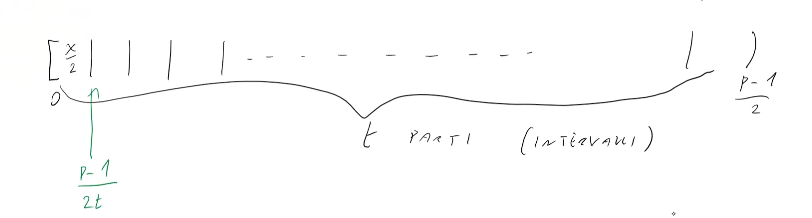
\includegraphics[width=1\textwidth]{images/7.png}
\end{center}
\noindent Supponiamo che $\frac{x}{2}$ sia nel primo intervallo. Qual è la probabilità di trovare un $r$ che vada bene? Se $r$ sta nell'ultimo intervallo, quello che termina con $\frac{p-1}{2}$, effettivamente è possibile che $\frac{x}{2} + r \not< \frac{p-1}{2}$. Ma se $r$ si trova in uno degli altri intervalli, non sarà mai possibile andare oltre $\frac{p-1}{2}$, in quanto il valore di $\frac{x}{2}$ non eccede la dimensione di un intervallo. Quindi la probabilità di trovare un $r$ che vada bene corrisponde alla probabilità di non finire nell'ultimo intervallo. Questa probabilità è:
\begin{align*}
    \frac{t-1}{t}
\end{align*}
\noindent ovvero la probabilità di essere in qualsiasi intervallo tranne l'ultimo. \\

\noindent Prendiamo l'esperimento completo:
\begin{itemize}
    \item Prendi $r$ a caso;
    \item Sia $a$ la PSQR di $yg^{2r}$;
    \item Ritorna $ag^{-r}$.
\end{itemize}
\noindent Scegliamo un $r$ a caso, produciamo il nuovo problema e ne calcoliamo la radice quadrata principale, da quella ricaviamo la risposta al problema originale. 

Qual è la probabilità che la risposta sia corretta? Affinché possiamo avere la garanzia che la risposta sia corretta, ci serve una risposta corretta la problema trasformato ($Pr = \frac{1}{2}k^{-c}$) e sapere di aver scelto una $r$ che soddisfa l'ipotesi del lemma ($Pr = \frac{t-1}{t}$). Quindi la probabilità è:
\begin{align*}
   \left(\frac{t-1}{t}\right) \left(\frac{1}{2}k^{-c}\right)
\end{align*}
\noindent Affinché il trucco di fare tanti esperimenti indipendenti e prendere il maggior numero di risposte corrette come risposta corretta funziona fintanto che la probabilità di dare la risposta corretta sia polinomialmente distante da $\frac{1}{2}$. Quindi la probabilità che avviamo travato deve essere:
\begin{align*}
   \left(\frac{t-1}{t}\right) \left(\frac{1}{2}k^{-c}\right) \ge \frac{1}{2}k^{-2c}
\end{align*}
\noindent Usiamo $k^{-2c}$ in quanto $\frac{t-1}{t}$ rende più piccolo $\left(\frac{1}{2}k^{-c}\right)$, e quindi sarà più vicino a $\frac{1}{2}$. Praticamente la nostra probabilità deve essere maggiore di $\frac{1}{2}$ di un qualsiasi polinomio, solo più piccolo del $k^{-c}$ che avevamo originariamente definito, in quanto sappiamo che $\frac{t-1}{t}$ riduce la nostra probabilità.

Abbiamo quindi imposto che questa grandezza sia sufficientemente distante da $\frac{1}{2}$. Se risolviamo la disequazione in $t$, riusciamo a trovare un limite inferiore al numero di intervalli da usare. Il limite inferiore che ci darà la disequazione sarà un limite polinomiale in $k$. 

Quindi dividendo per una quantità di intervalli che è polinomiale in $k$, riusciamo ad ottenere un sistema tale per cui se $x$ è nel primo intervallo, la probabilità di successo (di fornire una radice quadrata principale di $y$) è polinomialmente distante da $\frac{1}{2}$. Di conseguenza abbiamo un algoritmo polinomiale per calcolare la radice quadrata principale con probabilità di successo esponenzialmente vicina a $1$, grazie al limite di Chernoff.

Abbiamo costruito un algoritmo che con probabilità $\frac{1}{2}$ calcola il logaritmo discreto di un numero a patto che questo logaritmo discreto stia nel primo intervallo. Per portare la probabilità a $1$, basta ripetere l'algoritmo più volte. \\

\noindent Il problema ora è capire come costruire un algoritmo che funzioni su ogni intervallo a partire da uno che funziona con $x$ nel primo intervallo. 

Supponiamo di sapere che $\frac{x}{2}$ si trovi nell'intervallo $i$. L'intervallo i-esimo va da $i \cdot \frac{p-1}{2t}$ a $(i+1) \cdot \frac{p-1}{2t}$, supponendo di numerare gli intervalli con 0, 1, 2, ... . Prendiamo il nostro $y$ e lo moltiplichiamo per $g^{-\frac{p-1}{t}i}$. Cosa stiamo facendo? Sappiamo che $y=g^x$ e che $i \cdot \frac{p-1}{2t} \le \frac{x}{2} < (i+1) \cdot \frac{p-1}{2t}$, quindi se facciamo 
\begin{align*}
    g^{x'} = g^x g^{-\frac{p-1}{t}i}
\end{align*}
\noindent significa che
\begin{align*}
    \frac{x'}{2} = \frac{x - \frac{p-1}{t}i}{2} = \frac{x}{2} - \frac{p-1}{2t}i
\end{align*}

\noindent Con questa moltiplicazione (che diventa una sottrazione sugli esponenti) rimuoviamo il limite sinistro dell'intervallo, spostando il mostro problema dall'intervallo i-esimo al primo. Ci siamo quindi ricondotti al caso che il nostro algoritmo riesce a risolvere. Una volta che il nostro algoritmo avrà risolto il problema, basterà riaggiungere $\frac{p-1}{t}i$ al logaritmo discreto risultate per ottenere la risposta per l'intervallo i-esimo. 

Ci resta solo un problema: come possiamo risolvere il problema se non sappiamo in che intervallo ci troviamo? Basta provarli tutti, tanto sono una quantità polinomiale. Con il primo algoritmo visto siamo in grado di calcolare il logaritmo discreto con probabilità $\frac{1}{2}$ e verificare che sia corretto. Basta ripetere il test per ogni intervallo finché non ci troveremo in quello che rende vera l'ipotesi del lemma. Quindi l'algoritmo che testa una volta ognuna delle ipotesi finché non trova una risposta corretta sappiamo che ci darà la risposta corretta con probabilità almeno $\frac{1}{2}$. Se nessuna delle ipotesi ha dato la risposta corretta, basta ripetere il giro un'altra volta. IN un numero atteso di $2$ tentativi avremo la risposta corretta, il logaritmo discreto di $y$.
\end{proof}

\end{proof}
\end{proof}








































































\chapter{Generatori di bit pseudocasuali}
\label{chapter9}

Esiste un teorema generico che dice che ogni funzione one-way ammette hard core predicate. Se esistono le funzioni one-way allora esistono algoritmi per il lancio della moneta nel pozzo. Abbiamo dimostrato che gli algoritmi di lancio della moneta non esistono, in quanto c'è sempre un problema di sincronizzazione dei messaggi, ovvero esiste sempre un ultimo messaggio che può essere non spedito che impedisce all'altro agente di vedere il risultato del lancio. Si algoritmi per il lancio della moneta nel pozzo abbiamo visto quello basato sul residuo quadratico e quello basato sul logaritmo discreto.

Da quello basato sul logaritmo discreto abbiamo ricavato che in generale l'esistenza di funzioni one-way è la condizione sufficiente per l'esistenza di algoritmi di lancio nel pozzo.

Abbiamo dimostrato che la funzione one-way $g^x$ ammette hard core predicate $x < \frac{p-1}{2}$ in diversi passi:
\begin{itemize}
    \item Calcolare l'hard core predicate della funzione one-way equivale a calcolare la radice quadrata principale di un numero in $Z_p^*$. Quando abbiamo un quadrato (che sappiamo esserlo tramite il simbolo di Legendre), questo ammette due radici: quella aritmetica e il suo opposto. Ognuna di queste radici quadrata ha il suo logaritmo discreto, solo che non sappiamo quale delle due ha il logaritmo discreto più basso. Quindi il test del predicato binario ci permette capire quale dei due logaritmi discreti è nella prima metà e di conseguenza quale delle due radici è la principale.  Se abbiamo un sistema che calcola la radice quadrata principale di un numero, dato $x$ calcoliamo $x^2$ e lo passiamo in input al sistema: se ci ritorna il numero iniziale, allora $x$ è la radice quadrata principale, altrimenti basta prendere il suo opposto. 
    
    Abbiamo usato il calcolo della radice quadrata principale come base per mostrare che se esiste un algoritmo per l'hard core predicate allora esiste un algoritmo per il calcolo del logaritmo discreto (totale). Se noi partiamo col dire che calcolare il logaritmo discreto è difficile, allora deve essere difficile anche calcolare la radice quadrata principale e di conseguenza il calcolo di questo predicato binario.  
    
    Abbiamo scritto un algoritmo che calcola il logaritmo discreto di un numero partendo dal bit meno significativo e riconducendosi a calcolare il logaritmo discreto di un numero il cui logaritmo discreto è lo shift a destra dei bit del logaritmo discreto del numero originale. 
    Il logaritmo discreto di $1$ è banalmente $0$; il bit meno significativo del logaritmo discreto di $y$ è facile da calcolare con il simbolo di di Legendre. Se il bit è $1$ lo possiamo rendere $0$ dividendo per $g$ e ottenendo un nuovo numero il cui logaritmo discreto ha il bit meno significativo a $0$, cioè è un quadrato. Calcolando la radice quadrata principale del nuovo numero calcoliamo la radice discreta che è la divisione per $2$ del logaritmo discreto per $y$. Divisione per $2$ coincide con lo spostamento a destra di tutti i bit logaritmo discreto di $y$. A questo punto abbiamo il logaritmo discreto del numero ottenuto shiftando a destra tutti i bit del logaritmo discreto. Lo rishftiamo a sinistra moltiplicando per $2$ e aggiungiamo il bit meno significativo ottenendo il logaritmo discreto finale del numero $y$.
    
    \item Abbiamo detto che siamo in grado di calcolare il logaritmo discreto tramite il logaritmo che calcola la radice quadrata principale, ma noi non abbiamo un algoritmo per il calcolo della radice quadrata principale, ne abbiamo uno che la calcola a meno di un certo errore $\epsilon$. Se l'errore con cui calcoliamo la radice quadrata principale è $\epsilon$, qual è la probabilità di ottenere la risposta corretta con l'algoritmo descritto sopra? $(1-\epsilon)^k$, perché  calcolare $k$ radici quadrate principali e ogni calcolo deve dare la risposta corretta. 

    Vogliamo che l'errore finale sia non troppo alto, quindi $\epsilon$ deve essere molto piccolo. Per il teorema di analisi, se $\epsilon$ è esponenzialmente piccolo nel security parameter, allora la probabilità di successo è almeno $\frac{1}{2}$. Con questa probabilità abbiamo il vantaggio che reiterando più volte, in media dopo $2$ tentativi abbiamo la risposta corretta. 

    \item In realtà quando ci dicono che qualcuno è riuscito a rompere il protocollo di lancio della moneta, questo qualcuno ci dice che abbiamo in mano un algoritmo in grado di indovinare il predicato binario di qualche cosa con un vantaggio polinomiale rispetto ad $\frac{1}{2}$. Il nostro obiettivo è costruire un qualcosa che abbia un errore esponenzialmente piccolo. Per farlo basta costruire tanti esperimenti indipendenti per l'algoritmo $B$. Con esperimenti indipendenti intendiamo un problema nuovo che è distribuito esattamente secondo la distribuzione di probabilità che si aspetta l'algoritmo $B$ per dire che indovina con probabilità $\frac{1}{2} + \eta$. Questi esperimenti indipendenti devono essere tali che dalla risposta al nuovo esperimento sia possibile risalire alla risposta del problema originale. 

    Dobbiamo costruire un nuovo input $y'$ per la macchina $B$ tale per cui dalla risposta che diamo ad $y'$ siamo in grado di dare la risposta per $y$. Per costruire l'esperimento indipendente scegliamo un quadrato a caso e lo moltiplichiamo per $y$, ottenendo un quadrato a caso. L'algoritmo $B$ sarà in grado di calcolare il logaritmo discreto di $y'$ facilmente. Il quadrato a caso lo abbiamo costruito in modo da conoscere noi stessi il suo logaritmo discreto. Prima abbiamo calcolato il suo logaritmo discreto nella prima metà e poi abbiamo costruito il nuovo oggetto. L'oggetto lo vogliamo costruito in maniera tale che dalla risposta, ovvero dalla radice quadrata di questo oggetto, siamo in grado di trovare la radice quadrata principale di $y$.

    Il lemma che abbiamo dimostrato dice che questa cosa la sappiamo fare solo quando $x+2r < p-1$, ovvero quando nel calcolare i quadrati non andiamo oltre $p-1$ e non ci serve usare l'operazione di modulo (a livello di esponenti stiamo solo facendo un'operazione aritmetica). 

    Se $x+2r$ è sufficientemente piccolo riusciamo ad ottenere la risposta corretta. Ma a noi interessa ottenere sempre la risposta corretta. Più $x$ è piccolo, più è probabile scegliere un $r$ che funzioni.

    Abbiamo definito cosa significa per noi "essere piccolo": abbiamo diviso l'intervallo dei possibili logaritmi discreti in un numero di parti che non conosciamo $t$. Supponiamo che 
    $x$ stia nella prima delle $t$ parti e ci chiediamo quale sia la probabilità di trovare un $r$ che vada bene per il lemma. Questa probabilità è equivalente alla probabilità di avere un $r$ che stia in tutti gli intervalli eccetto l'ultimo. Solo quando  $r$ sta nell'ultimo intervallo, rischiamo di uscire dal limite se aggiungiamo la nostra $x$.
    La probabilità di andare in tutti gli intervalli eccetto l'ultimo è $\frac{t-1}{t}$. A questo punto abbiamo potuto calcolare qual è la probabilità di ottenere la risposta corretta all'esperimento completo: trasformare il problema, prendere la risposta al problema trasformato, dividerla per $g^r$ per ottenere la risposta al problema originale.

    La probabilità che abbiamo trovato è un limite inferiore in quanto $\frac{t-1}{t}$ non comprende anche quegli $r$ appartenenti all'ultimo intervallo che andrebbero comunque bene. Al fine di usare il teorema di Chernoff e poter fare un numero polinomiale di esperimenti per avere la probabilità esponenzialmente vicina ad $1$ di avere la risposta corretta, la nuova probabilità deve essere polinomialmente distante da $\frac{1}{2}$. 

    Scegliamo quindi un polinomio che ci vada bene, tipo $k^{-2c}$, e verifichiamo se riusciamo a trovare una soluzione alla disequazione che si genera con la probabilità di successo dell'esperimento. La soluzione ci determina il numero (polinomiale in $k$) minimo di intervalli in cui dobbiamo dividere il numero di logaritmi discreti. Se non ci riusciamo, non siamo in grado di dimostrare che abbiamo un vantaggio polinomiale. 

    In questo modo, con una quantità polinomiale in $k$ di intervalli, abbiamo la garanzia di poter essere polinomialmente distante da $\frac{1}{2}$ con il nuovo esperimento. Grazie a questo possiamo avere la risposta corretta con probabilità esponenzialmente vicina ad $1$ e quindi possiamo arrivare a calcolare il logaritmo discreto con probabilità almeno $\frac{1}{2}$.

    Ma se $x$ non si trova nel primo intervallo e qualcuno ci dice dove sta? Possiamo moltiplicare $y$ per una quantità opportuna tale per cui il nuovo logaritmo discreto sta nel primo intervallo. 

    Ma se non sappiamo in che intervallo si trova $x$? Grazie al fatto che il numero di intervalli è polinomiale in $k$, possiamo provare la nostra ipotesi in ciascun intervallo. Prima o poi la proveremo in quello corretto e con probabilità $\frac{1}{2}$ avremo in mano il nostro logaritmo discreto. Se una volta provati tutti li intervallo non avremo trovato il logaritmo discreto, ritentiamo un'altra volta (con probabilità $\frac{1}{2}$ potremo non trovarlo). In media con $2$ tentativi ce la facciamo. 
\end{itemize}

\section{Bit pseudocasuali}
Vogliamo costruire una sequenza di bit che sia equivalente all'aver lanciato una moneta ogni volta. All'interno di un computer non vi è nulla di casuale, è tutto deterministico. Se conosciamo lo stato del pc, possiamo prevedere tutto quello che farà. Vogliamo fare in modo che il pc possa generare una serie di bit in modo deterministico che appaiano casuali a chi li osserva (per questo sono chiamato pseudocasuali).

La nostra generazione di bit pseudocasuali non può essere un processo semplice che costruisce qualcosa distribuito uniformemente, ma deve essere un qualcosa che produce una sequenza di bit tale che nessuno con potenza di calcolo probabilistica polinomiale sia in grado di capirla. 

Vogliamo un sistema PRSG (Pseudo Random Sequence Generator) che dato in input un seme di dimensione $k$ produce in output una sequenza di bit di lunghezza $l$, con $l>k$, tale che nessuno che osserva la sequenza riesca a dire che non è propriamente casuale. Il seme è scelto in maniera realmente casuale. Questi generatori da un seme iniziale producono una sequenza di bit maggiore la cui difficoltà di identificazione cresce al crescere di $k$. Più bit usiamo per il seme iniziale, più difficile è capire che la sequenza generata non è casuale. 

I generatori che andremo a costruire li possiamo vedere come moltiplicatori di casualità: a partire da una casualità vera, il seme, andremo a generare una casualità più grande rispetto a quella originale. I bit che genereremo saranno tali per cui nessun algoritmo PPT riesca a trovare regolarità al suo interno. Della regolarità esiste, noi saremmo in grado di rappresentare la sequenza in maniera più compatta, ma nessun algoritmo PPT deve essere in grado di trovare questa regola. 


\noindent Cosa vuol dire generare bit pseudocasuali?  Se riceviamo $b_0, b_1, ..., b_l$ facciamo fatica ad indovinare $b_{l+1}$, ovvero lo indoviniamo con vantaggio più piccolo di ogni polinomio. Quindi la probabilità  $P[\Sigma]$ di:
\begin{itemize}
    \item Prendiamo il seme $S \in \{0, 1\}^k$ e la sequenza $b_1, ..., b_l, b_{l+1}$ generata dal generatore $G(S)$;
    \item Prendiamo $b$ ottenuto dall'algoritmo $A(b_1, ..., b_l)$, che tenta di predire il bit successivo a partire dalla sequenza $(b_1, ..., b_l$;
    \item Verifichiamo se $b == b_{l+1}$.
\end{itemize}

\noindent deve essere:
\begin{align}
    \left|P[\Sigma] - \frac{1}{2} \right| < k^{-\omega(1)}
\end{align}

\noindent Questa formula determina quando il generatore pseudocasuale è corretto, ovvero quando un attaccante non è capace di indovinare il bit successivo conoscendo i bit precedenti. 

\section{Generazione di bit pseudocasuali basata sulla difficoltà del logaritmo discreto}
Vediamo ora un algoritmo per la generazione di bit pseudocasuali basato sulla difficoltà del logaritmo discreto:
\begin{enumerate}
    \item Fissiamo $p, g$;
    \item Prendiamo il seme $x \in_R \{0, p-1\}$;
    \item Definiamo:
        \begin{center}
            \begin{tabular}{ c c c c c c }
              $a_0$ & $a_1$ & $a_2$ & $a_3$ & $...$ & $a_l$\\
              \vspace{1cm}
              $x$ & $g^x$ & $g^{g^x}$ & $g^{g^{g^x}}$ & $...$ & $g^{g^{.^{.^{g^x}}}}$  
            \end{tabular}
        \end{center}
    In maniera compatta questo può essere riscritto come:
    \begin{align*}
         \begin{cases}
            a_{i+1} &= g^{a_i}\\
            a_0 &= x
        \end{cases}
    \end{align*}

    Stiamo generando una sequenza di elementi $a_0, a_1, ...$ di $Z_p^*$, dove il primo elemento è il nostro seme, e ogni elemento successivo non è altro che il generatore elevato all'elemento precedente.

    \item Definiamo ora i nostri bit:
    \begin{center}
            \begin{tabular}{ c c c c c c }
              $a_0$ & $a_1$ & $a_2$ & $a_3$ & $...$ & $a_l$\\
              \vspace{1cm}
              $x$ & $g^x$ & $g^{g^x}$ & $g^{g^{g^x}}$ & $...$ & $g^{g^{.^{.^{g^x}}}}$\\
              \vspace{1cm}
              $b_0$ & $b_1$ & $b_2$ & $b_3$ & $...$ & $b_l$\\
            \end{tabular}
        \end{center}
    dove:
    \begin{align*}
         b_i = \begin{cases}
            0 & \mbox{se } a_i < \frac{p-1}{2}\\ 
            1 & \mbox{altrimenti}
        \end{cases}
    \end{align*}

    \item Ritorniamo la sequenza
    \begin{align*}
        b_{l} \ b_{l-1} \ b_{l-2} \ ... \ b_{1} \ b_{0}
    \end{align*}
       
\end{enumerate}

\begin{proof}[Dimostrazione di correttezza]
    Supponiamo per assurdo che esiste un algoritmo in grado di predire il successivo. Questo algoritmo prende in input una quantità di bit e indovina il bit successivo con un vantaggio che è più grande di qualche polinomio. 

    Supponiamo che dati in input i bit $b_l \ ... \ b_3$ ($l-3$ bit) l'algoritmo riesca ad indovinare il bit $b_2$. 

    Se osserviamo la sequenza notiamo che:
    \begin{itemize}
        \item $b_2$ è l'hard core predicate di $a_3$:
        \begin{align*}
            a_3 &= g^{a_2}\\
            b2 &= hcp(a_2)
        \end{align*}
        \item $a_2$ è il logaritmo discreto di $a_3$:
        \begin{align*}
            a_3 &= g^{a_2}\\
           DL(a_3) &= DL(g^{a_2}) = a_2
        \end{align*}
    \end{itemize}

    \noindent Se noi abbiamo $a_3$, calcolare $b_2$ vuol dire calcolare l'hard core predicate di $a_3$. Dimostriamo ora che se abbiamo un algoritmo che indovina $b_2$ a partire dalla sequenza $b_l \ ... \ b_3$ con vantaggio polinomiale, allora abbiamo un algoritmo che calcola l'hard core predicate con vantaggio polinomiale. 

    Preso in input il numero, lo vediamo come se fosse $a_3$ e generiamo la sequenza fino ad $a_l$. Generati questi oggetti, possiamo costruire la sequenza $b_l \ ... \ b_3$. Applichiamo l'algoritmo che indovina $b_2$. L'algoritmo indovina con vantaggio polinomiale rispetto a $\frac{1}{2}$, cioè abbiamo calcolato l'hard core predicate di $a_3$ con vantaggio polinomiale rispetto a $\frac{1}{2}$.

    L'eventuale previsione del bit successivo diventa il calcolo dell'hard core predicate (fino all'ottenimento del seme). L'algoritmo che abbiamo costruito restituisce i bit alla rovescia in quanto altrimenti il bit successivo della sequenza sarebbe stato il risultato di una funzione facile da calcolare. Noi abbiamo usato una funzione difficile da calcolare sui semi per dire che non riusciamo a indovinare il bit successivo. Restituirli alla diritta equivale a calcolare una funzione one-way, che sappiamo calcolare, per ottenere il bit successivo.

    Restituendo i bit alla diritta questa dimostrazione non avrebbe funzionato. Ma questo significa che non è possibile restituire i bit alla diritta? No, se noi non siamo capaci di trovare una dimostrazione per qualcosa, non significa che quel qualcosa sia falso. La nostra dimostrazione del protocollo alla rovescia si basa sul fatto che conoscendo i semi non siamo in grado di calcolare $b_2$. Se non siamo in grado di calcolarlo conoscendo i semi, a maggior ragione non siamo in grado di calcolarlo conoscendo i bit. Se conosciamo solo bit, siamo molto più in difficoltà, ma questa dimostrazione non ci permette di catturare questo concetto. 


    Definizione con distinguisher:
    \begin{align*}
        \forall D \in PPT \ \forall l&\\
        P_K^{D, G} &= Pr[S \in_R \{0, 1\}^k; b_0 \ ... \ b_l \leftarrow G(S); D(b_1 \ ... \ b_l) == 1]\\
        P_K^{D, U} &= Pr[S \in_R \{0, 1\}^{l+1}; D(b_0 \ ... \ b_l) == 1]\\
        \left|P_K^{D, G} - P_K^{D, U}\right| &< k^{-\omega(1)}
    \end{align*}



    \noindent Se $b_l \ ... \ b_0$ soddisfa la definizione di indovinare allora soddisfa anche la definizione di distinguere, quindi la sequenza $b_l \ ... \ b_0$ è indistinguibile da una sequenza casuale. 

    Possiamo di conseguenza che $b_0 \ ... \ b_l$ sia indistinguibile? Sia $D$ un distinguisher per $b_l \ ... \ b_0$ (che distingue tra una sequenza veramente casuale e non) e sia $D'$ una macchina tale per cui:
    \begin{align*}
        D' :& b_l \ ... \ b_0 \rightarrow D(b_0 \ ... \ b_l)\\
            & b_0 \ ... \ b_l \rightarrow D(b_l \ ... \ b_0)
    \end{align*}

    \noindent Se $D'$ riesce a distinguere i bit diritti, vuol dire che $D$ sta distinguendo o bit rovesci; se $D'$ riesce a distinguere i bit rovesci, vuol dire che $D$ sta distinguendo o bit diritti. Quindi distinguere i bit rovesci o dritti è la stessa cosa: se abbiamo distinguisher per i bit rovesci basta invertire i bit dati in input e costruiamo un distinguisher per i bit diritti.

    Con la definizione di indovinare siamo riusciti a dimostrare che i bit alla rovescia funzionano, ma non per i bit diritti. Grazie all'equivalenza tra indovinare e distinguere siamo riusciti a dimostrare che anche i bit diritti funzionano.

    Il vantaggio di restituire i bit alla rovescia sta nel fatto che dopo aver ritornato $b_0$ non siamo in grado di andare avanti con la sequenza: per ottenere il bit successivo dovremmo calcolare il logaritmo discreto del seme (non siamo in grado di calcolare il logaritmo discreto). Il vantaggio dei bit diritti sta nel fatto che possiamo generare bit ogni volta che sono richiesti (dimensione arbitraria).
\end{proof} 

\subsection{Indovinare $\leftrightarrow$ Distinguere}
\begin{proof}[indovinare $\rightarrow$ distinguere]
    Su input $b_0 \ ... \ b_{l-1}$ indoviniamo $b_l$ con vantaggio polinomiale:
    \begin{align*}
        \left|Pr[A(b_0 \ ... \ b_{l-1}) = b_l] - \frac{1}{2}\right| > k^{-\omega(1)}
    \end{align*}

    \noindent Quindi
    \begin{align*}
        Pr[A(b_0 \ ... \ b_{l-1}) = b_l]   > \frac{1}{2} + k^{-\omega(1)}
    \end{align*}

    \noindent Per dimostrare che violando la definizione di indovinare violiamo quella di distinguere possiamo costruire un distinguisher che:
    \begin{align*}
        D(b_0 \ ... \ b_{l}) = 
        \begin{cases} 
        1 & \mbox{se } A(b_0 \ ... \ b_{l-1}) = b_l \\ 
        0 & \mbox{altrimenti }
        \end{cases} 
    \end{align*}

    \noindent A partire dall'algoritmo $A$ che attacca il sistema di generazione dei bit pseudocasuali secondo la definizione di indovinare, cerchiamo di costruire un distinguisher che distingue sequenza casuali da pseudocasuali.

    Vediamo qual è la probabilità che l'algoritmo $A$ indovini un bit che viene scelto in modo veramente casuale e indipendente da $b_0 \ ... \ b_{l-1}$. Noi sappiamo che se c'è un qualsiasi algoritmo che genera un bit e lo mettiamo in XOR con un bit veramente casuale, la probabilità di uguaglianza è esattamente $\frac{1}{2}$. Quindi la probabilità che $A(b_0 \ ... \ b_{l-1}) = b_l$ è esattamente $\frac{1}{2}$:
    \begin{align}
        P_k^{D, U} = \frac{1}{2}
    \end{align}

    \noindent Sappiamo che la probabilità che $A$  indovini $b_l$ è:
    \begin{align}
        P_k^{D, G} = Pr[A(b_0 \ ... \ b_{l-1}) = b_l] > \frac{1}{2} + k^{-c}
    \end{align}

    \noindent Di conseguenza
    \begin{align}
        P_k^{D, G} - P_k^{D, G} \gw \frac{1}{2} + k^{-c} - \frac{1}{2} = k^{-c}
    \end{align}

    \noindent La differenza tra le due probabilità è maggiore del polinomio $k^{-c }$. Di conseguenza. Quindi se abbiamo l'attaccante per la definizione di indovinare abbiamo anche il distinguisher per la definizione di distinguere. 
\end{proof}

\begin{proof}[indovinare $\rightarrow$ distinguere]
    Date la sequenza $b_1 \ ... \ b_{l}$ pseudocasuale e la sequenza $r_1 \ ... \ r_{l}$ casuale, sia $D$ distinguisher che vede al differenza tra le due. Con queste due sequenza non possiamo fare molto per proseguire con la dimostrazione. 
    
    Definiamo la sequenza $S_i = b_1 \ ... \ b_i \ R_{i+1} \ ... \ r_l$. Allora $S_0$ è la sequenza pseudocasuale e $S_l$ è la sequenza casuale. 

    Definiamo $P_i$ come la probabilità che $D$ restituisca $1$ con input $S_i$; allora $P_0 = P_k^{D, R}$ e $P_l = P_k^{D, G}$.
    Sapendo che $|P_l - P_0| > k^{-c}$, facendo la costruzione per interpolazione arriviamo a dire che
    \begin{align*}
        \exists i \ |P_i - P_{i+1}| > k^{-c}
    \end{align*}

    \noindent Cerchiamo ora di definire $A$ che predice il bit $i+1$ conoscendo i bit precedenti:
    \begin{align*}
        A(b_1 \ ... \ b_l) = 
        \begin{cases} 
        R_{i+1} & \mbox{se } D(b_1 \ ... \ b_i \ R_{i+1} \ ... \ r_l) = 1 \\ 
        \overline{R_{i+1}} & \mbox{se } D(b_1 \ ... \ b_i \ R_{i+1} \ ... \ r_l) = 0
        \end{cases} 
    \end{align*}

    \noindent Vediamo ora qual è la probabilità che $Pr[A(b_1 \ ... \ b_{l}) = b_{l+1}]$:
    \begin{align*}
        Pr[A(b_1 \ ... \ b_{l}) = b_{l+1}] = Pr[R_{i+1} = b_{b+1}] \cdot P_{i+1} +  Pr[R_{i+1} = \overline{b_{b+1}}] \cdot X
    \end{align*}

    \noindent Quando $A$ indovina? Distinguiamo sul valore di $R_{i+1}$: la probabilità di indovinare è data dalla probabilità di indovinare quando il bit successivo è generato ($b_{i+1}$) sommata alla probabilità di indovinare quando il bit è casuale.
    Se il bit successivo è quello pseudogenerato, la probabilità di indovinare è $P_{i+1}$, ovvero la probabilità che il distinguisher dia $1$ quando sappiamo che i primi $i+1$ bit sono generati (sequenza $b_1 \ ... \ b_i \ b_{i+1} \ r_{i+2} \ ... \ r_l$); se il bit successivo è casuale, la probabilità di indovinare è $X$, che è la probabilità che restituisca $0$ sulla sequenza $b_1 \ ... \ b_i \ \overline{b_{i+1}} \ r_{i+2} \ ... \ r_l$.

    Procediamo col calcolo della probabilità. Poiché il bit $b_{i+1}$ è scelto in maniera casuale, la probabilità che sia $r_{i+1}$ è esattamente $\frac{1}{2}$:
    \begin{align*}
        Pr[A(b_1 \ ... \ b_{l}) = b_{l+1}] = \frac{1}{2} P_{i+1} + \frac{1}{2} X
    \end{align*}

    \noindent Proviamo ora a capire che relazione esiste tra $X$, $P_{i+1}$ e $P_i$. Vediamo quanto vale $P_i$, ovvero la probabilità che $D$ restituisca $1$ con input la sequenza con bit i-esimo casuale, e i successivi pseudocasuali:
    \begin{align*}
        P_{i} = &Pr[\textbf{bit $i+1$} = b_{i+1}] \codt Pr[D\text{ dia $1$ su } b_1 \ ... \ b_i \ b_{i+1} \ ... \ b_l] + \\
        &Pr[\textbf{bit $i+1$} = \overline{b_{i+1}}] \codt Pr[D\text{ dia $1$ su } b_1 \ ... \ b_i \ \overline{ b_{i+1}} \ ... \ b_l]
    \end{align*} 

    \noindent Risolvendo:
    \begin{align*}
        P_{i} = &\frac{1}{2}P_{i+1} + \frac{1}{2} (1-X)
    \end{align*}

    \noindent Da questa formula ricaviamo che
    \begin{align*}
        X = 1 - (2P_i - P_{i+1})
    \end{align*}

    \noindent Risolvo $X$ nell'espressione sopra:
    \begin{align*}
        Pr[A(b_1 \ ... \ b_{l}) = b_{l+1}] &= \frac{1}{2} P_{i+1} + \frac{1}{2} X\\
        &= \frac{1}{2} P_{i+1} + \frac{1}{2} (1 - (2P_i - P_{i+1}))\\
        &= \frac{1}{2} P_{i+1} + \frac{1}{2} - P_i + \frac{1}{2} P_{i+1}\\
        &= \frac{1}{2} + P_{i+1} - P_i\\
        Pr[A(b_1 \ ... \ b_{l}) = b_{l+1}] - \frac{1}{2} &= P_{i+1} - P_i
    \end{align*}

    \noindent Di conseguenza
    \begin{align*}
        \left|\underbrace{Pr[A(b_1 \ ... \ b_{l}) = b_{l+1}]}_{Pr[A \text{ corretto}]} - \frac{1}{2} \right| &= \left|P_{i+1} - P_i \right| \ge k^{-c}
    \end{align*}

    \noindent Abbiamo dimostrato che 
\end{proof}

\section{Algoritmo di Blum Blum Shoup}
Algoritmo per la generazione di bit pseudocasuali basato sulla difficoltà del calcolo di radici quadrate in $Z_n^*$. La funzione elevamento al quadrato in $Z_{pq}^*$ è una funzione one-way trapdoor. Sappiamo che l'inversione equivale a fattorizzare (dimostrazione $MCD(x+y, n)$). Se conosciamo $p, q$ allora sappiamo calcolare le radici.

\begin{theorem}[Primi di Blum]
    Se 
    \begin{align*}
        p, q \equiv 3 \pmod 4
    \end{align*}
    \noindent allora per ogni quadrato $x$ esiste un'unica radice che un quadrato
\end{theorem}

\noindent L'hard core predicate che usiamo per la radice quadrata è il $LSB(\sqrt{x})$, quando vale il teorema sopra.\\

\noindent Vediamo l'algoritmo:
\begin{itemize}
    \item Sia $n = pq$ con $p, q$ primi di Blum scelti a caso;
    \item Sia $x \in_R Z_n^*$;
    \item Definiamo:
    \begin{center}
            \begin{tabular}{ c c c c c }
              $a_1$ & $a_2$ & $a_3$ & $...$ & $a_l$\\
              \vspace{1cm}
              $x^2$ & ${(x^2)}^2$ & ${({(x^2)}^2)}^2$ & $...$ & ${x^2}^{l}$\\
            \end{tabular}
        \end{center}

    \noindent dove:
    \begin{align*}
         \begin{cases}
            a_1 &= x^2\\ 
            a_{i+1} &= a_i^2
        \end{cases}
    \end{align*}

    \noindent Stiamo applicando successivamente la nostra funzione one-way trapdoor. Definiamo $b_i = LSB(a_i)$:
    \begin{center}
            \begin{tabular}{ c c c c c }
              $a_1$ & $a_2$ & $a_3$ & $...$ & $a_l$\\
              \vspace{1cm}
              $x^2$ & ${(x^2)}^2$ & ${({(x^2)}^2)}^2$ & $...$ & ${x^2}^{l}$\\
              $b_1$ & $b_2$ & $b_3$ & $...$ & $b_l$\\
            \end{tabular}
        \end{center}
    \item Restituiamo i bit $b_l \ ... \ b_1$.
        
\end{itemize}

\section{Sistema a chiave pubblica dimostrabilmente sicuro - Algoritmo di Blum Goldwasser}
\textbf{Generazione chiavi} 
\begin{itemize}
    \item $p, q \in_R $ primi di Blum con $k$ bit;
    \item $n = pq$;
    \item $P_k = n$, $S_n=(p, q)$.
\end{itemize}

\noindent \textbf{Encryption}
\begin{itemize}
    \item Vogliamo cifrare il messaggio $m: \ m_1 \ ... \ m_l$;
    \item $x \in Z_n^*$;
    \item Usiamo Blum Blum Shoup (BBS) per generare $l$ bit pseudocasuali:
    \begin{center}
            \begin{tabular}{ c c c c c c c }
              & $x^2$ & ${(x^2)}^2$ & ${(x^2)}^3$ & $...$ & ${x^2}^{l}$ & \\
              & $b_1$ & $b_2$ & $b_3$ & $...$ & $b_l$ & \\
              $\bigoplus$ & $m_1$ & $m_2$ & $m_3$ & $...$ & $m_l$ & \\
              \hline
              & $c_1$ & $c_2$ & $c_3$ & $...$ & $c_l$ & ${x^2}^{(l+1)}$ \\
            \end{tabular}
        \end{center}

        \noindent Abbiamo usato one-time pad con una chiave che è pseudogenerata a partire da un seme scelto a caso. Questo protocollo è praticamente one-time pad. Noi sappiamo che se la sequenza $b_1 \ ... \ b_l$ è veramente casuale, allora il cyphertext non contiene alcuna informazione circa il plaintext (quindi il cyphertext costruito è completamente sicuro).

        Supponiamo che qualcuno riesca a ottenere qualcosa dal cyphertext, che riesca a distinguere qualsiasi coppia di messaggi cifrata con questo sistema. Quel qualcuno che riesce a vedere se due cyphertext sono dello stesso messaggio o di messaggi diversi sappiamo che non lo riesce a fare in presenza di una chiave veramente casuale. Quel distinguisher per due messaggi del nostro crittosistema diventerebbe un distinguisher per un generatore di bit pseudocasuali: se sono veramente pseudocasuali $D$ non distingue, se i bit sono pseudocasuali si comporta in maniera diversa. Questa macchina diventa un distinguisher per Blum Blum Shoup, che soddisfa 
\end{itemize}


















\chapter{Protocolli vari}
\label{chapter1}

 










\end{document}